% SIAM Article Template
\documentclass[onefignum,onetabnum,dvipsnames]{siamart220329}

% Information that is shared between the article and the supplement
% (title and author information, macros, packages, etc.) goes into
% ex_shared.tex. If there is no supplement, this file can be included
% directly.
\setcounter{tocdepth}{2} % optional—include subsections

% SIAM Shared Information Template
% This is information that is shared between the main document and any
% supplement. If no supplement is required, then this information can
% be included directly in the main document.

% Packages and macros go here
\usepackage{algorithm}
\usepackage{algpseudocode}
\usepackage{algorithmicx}
\usepackage{amsfonts, amsmath, amsopn, amssymb}
\usepackage[american]{babel}
\usepackage[nameinlink]{cleveref}
\usepackage{csquotes}
\usepackage{enumitem}
\usepackage{epstopdf}
\usepackage{graphicx}
\ifpdf
  \DeclareGraphicsExtensions{.eps,.pdf,.png,.jpg}
\else
  \DeclareGraphicsExtensions{.eps}
\fi
\usepackage{tikz}
% Add a serial/Oxford comma by default.
\newcommand{\creflastconjunction}{, and~}

\usepackage[normalem]{ulem}
\usepackage[backgroundcolor=orange,textcolor=white,linecolor=gray,textsize=footnotesize]{todonotes}
\makeatletter% 
\@mparswitchfalse%
\makeatother%
\normalmarginpar%
\setlength{\marginparwidth}{5cm}

% Used for creating new theorem and remark environments
\newsiamremark{remark}{Remark}
\newsiamremark{hypothesis}{Hypothesis}
\crefname{hypothesis}{Hypothesis}{Hypotheses}
\newsiamthm{claim}{Claim}

\crefname{subsection}{section}{sections}
\Crefname{subsection}{Section}{Sections}
\crefname{subsubsection}{section}{sections}
\Crefname{subsubsection}{Section}{Sections}

%%%%%%%%%%%%%%%%%%%%%%%%
%% AUTHOR INFORMATION %%
%%%%%%%%%%%%%%%%%%%%%%%%
\usepackage{verbatim}
\begin{comment}

\newcommand{\theauthor}{Kai Bergermann}
\newcommand{\theorcid}{0000-0002-2259-1839}
\newcommand{\theaffiliation}{%
Department of Mathematics,
Technische Universität Chemnitz,
09107 Chemnitz,
Germany}
\newcommand{\theemail}{kai.bergermann@math.tu-chemnitz.de}

\newcommand{\theauthor}{Massimiliano Fasi}
\newcommand{\theorcid}{0000-0002-6015-391X}
\newcommand{\theaffiliation}{%
School of Computing,
University of Leeds,
Woodhouse Lane,
Leeds LS2 9JT,
United Kingdom}
\newcommand{\theemail}{m.fasi@leeds.ac.uk}

\newcommand{\theauthor}{Stéphane Gaudreault}
\newcommand{\theorcid}{0000-0002-4475-0845}
\newcommand{\theaffiliation}{%
Recherche en prévision numérique atmosphérique,
Environnement et Changement climatique Canada,
2121 Route Transcanadienne,
Dorval, Québec, H9P 1J3,
Canada}
\newcommand{\theemail}{stephane.gaudreault@ec.gc.ca}

\newcommand{\theauthor}{Xiaobo Liu}
\newcommand{\theorcid}{0000-0001-8470-8388}
\newcommand{\theaffiliation}{%
Max Planck Institute for Dynamics of Complex Technical Systems,
Sandtorstr.~1,
29106 Magdeburg,
Germany}
\newcommand{\theemail}{xliu@mpi-magdeburg.mpg.de}

\newcommand{\theauthor}{Kathryn Lund}
\newcommand{\theorcid}{0000-0001-9851-6061}
\newcommand{\theaffiliation}{%
Computational Mathematics Theme,
Scientific Computing Department,
STFC Rutherford Appleton Laboratory,
Didcot OX11 0QX,
United Kingdom}
\newcommand{\theemail}{kathryn.lund@stfc.ac.uk}

\newcommand{\theathor}{Stefano Pozza}
\newcommand{\theorcid}{0000-0003-1529-8420}
\newcommand{\theaffiliation}{%
Department of Numerical Mathematics,
Faculty of Mathematics and Physics,
Charles University,
Sokolovsk\'a 83,
186 75 Praha 8,
Czechia}
\newcommand{\theemail}{pozza@karlin.mff.cuni.cz}

\newcommand{\theauthor}{Marcel Schweitzer}
\newcommand{\theorcid}{0000-0002-4937-2855}
\newcommand{\theaffiliation}{%
School of Mathematics and Natural Sciences,
Bergische Universität Wuppertal,
42097 Wuppertal,
Germany}
\newcommand{\theemail}{marcel@uni-wuppertal.de}

\end{comment}

%%%%%%%%%%%%%%%%%%%%%%%%%%%%
%% MANUSCRIPT INFORMATION %%
%%%%%%%%%%%%%%%%%%%%%%%%%%%%

\newcommand{\thetitle}{Computing the action of matrix functions%
  \thanks{Submitted to the editors DATE. %
    \funding{This work was funded by \dots}}}
\newcommand{\theshorttitle}{Computing the action of matrix functions}
\newcommand{\theshortauthor}{Short names}

\newcommand{\thededication}{This work is dedicated to the memory of Nicholas J.~Higham (1961--2024).}

\newcommand{\theabstract}{\todo[inline]{KL: Write abstract}}

\newcommand{\theacks}{}

\newcommand{\thekeywords}{matrix function times a vector, matrix functions, numerical linear algebra, iterative methods, Krylov subspace method, polynomial approximation, rational approximation}

\newcommand{\themsc}{%
  15A16, % Matrix exponential and similar functions of matrices
  15-11, % Research data for problems pertaining to linear algebra
  65F60, % Numerical computation of matrix exponential and similar matrix functions
  65Y20, % Complexity and performance of numerical algorithms
  65-11  % Research data for problems pertaining to numerical analysis
}

%%%%%%%%%%%%%%%%%%%%%%%%%
%% COMMENTS AND TO-DOs %%
%%%%%%%%%%%%%%%%%%%%%%%%%

\usepackage{tcolorbox}
\newcommand{\MF}{Max}
\tcbuselibrary{skins}
\tcbuselibrary{breakable}
\tcbset{shield externalize}
\newenvironment{mf}{%
	\list{}{\leftmargin0.2cm\rightmargin\leftmargin}\item\relax%
	\begin{tcolorbox}[breakable, %
		colback=Red!10!white, sharp corners, boxrule=0pt,frame hidden, %
		enhanced, borderline west={1mm}{-2mm}{Green}]%
		\small\sffamily{\color{Green}\textbf{\MF:}}}
	{\end{tcolorbox}\endlist}

\newcommand{\KL}{Kathryn}
\newenvironment{kl}{%
	\list{}{\leftmargin0.2cm\rightmargin\leftmargin}\item\relax%
	\begin{tcolorbox}[breakable, %
		colback=Violet!10!white, sharp corners, boxrule=0pt,frame hidden, %
		enhanced, borderline west={1mm}{-2mm}{Violet}]%
		\small\sffamily{\color{Violet}\textbf{\KL:}}}
	{\end{tcolorbox}\endlist}

% Other macros
\newcommand{\ghissue}[1]{\href%
	{https://github.com/fAbsuite/fAbsurvey/issues/#1}
	{{issue #1}}}

\def\showcomments{1}
\ifx\showcomments\undefinded
\usepackage{environ}
\NewEnviron{killcontents}{}
\let\mf\killcontents
\let\endmf\endkillcontents
\let\kl\killcontents
\let\endkl\endkillcontents
\fi

%%% Local Variables:
%%% mode:latex
%%% TeX-master: "main"
%%% End:

\usepackage{amsopn, bm}
% Special math commands
% ----------------------------------------------------------------------------
\usepackage[mathscr]{euscript}
\DeclareMathOperator{\trace}{trace}
\DeclareMathOperator{\diag}{diag}
\DeclareMathOperator{\blkdiag}{blkdiag}
\DeclareMathOperator{\spn}{span}	% span of vectors
\DeclareMathOperator{\blkspn}{span^\square}
\DeclareMathOperator{\colspn}{colspan}
\DeclareMathOperator{\spnS}{\spn^{\mathbb{S}}}
\DeclareMathOperator{\rnk}{rank}
\DeclareMathOperator{\spec}{spec}	% spectrum of a matrix
\DeclareMathOperator{\sign}{sign}	% the sign function
\DeclareMathOperator{\nnz}{nnz}


%% Standard notation for... %%------------------------------------------
% Spaces
\newcommand{\spC}{\mathbb{C}}				% field of complex scalars
\newcommand{\spCpos}{\mathbb{C}^+}				% field of complex scalars
\newcommand{\spD}{\mathbb{D}}				% generic domain
\newcommand{\spEK}{\mathcal{E}}				% Krylov subspace in \spC^{n}
\newcommand{\spK}{\mathcal{K}}				% Krylov subspace in \spC^{n}
\newcommand{\spQ}{\mathcal{Q}}				% Rational Krylov subspace in \spC^{n}
\newcommand{\spKblk}{\mathcal{K}^{\square}}	% block Krylov subspace in \spC^{n}
\newcommand{\spP}{\mathbb{P}}				% space of polynomials
\newcommand{\spR}{\mathbb{R}}				% field of real scalars
\newcommand{\spU}{\mathcal{U}}				% vector space
\newcommand{\spV}{\mathcal{V}}				% vector space
\newcommand{\spW}{\mathcal{W}}				% vector space

% Scalars (lowercase Greek, no style)
\newcommand{\thetatil}{\widetilde{\theta}}

% Block scalars (uppercase Greek, no style)


% Matrix components (lowercase Roman, no style)


% Block matrix components (uppercase Roman, no style)


% Vectors (bold lowercase Roman)
\newcommand{\va}{\bm{a}}
\newcommand{\vb}{\bm{b}}
\newcommand{\vd}{\bm{d}}
\newcommand{\ve}{\bm{e}}
\newcommand{\vehat}{\widehat{\ve}}
\newcommand{\vf}{\bm{f}}
\newcommand{\vg}{\bm{g}}
\newcommand{\vh}{\bm{h}}
\newcommand{\vk}{\bm{k}}
\newcommand{\vp}{\bm{p}}
\newcommand{\vq}{\bm{q}}
\newcommand{\vr}{\bm{r}}
\newcommand{\vs}{\bm{s}}
\newcommand{\vu}{\bm{u}}
\newcommand{\vv}{\bm{v}}
\newcommand{\vvhat}{\widehat{\vv}}
\newcommand{\vw}{\bm{w}}
\newcommand{\vx}{\bm{x}}
\newcommand{\vy}{\bm{y}}
\newcommand{\vz}{\bm{z}}
\newcommand{\vone}{\boldsymbol{1}}
\newcommand{\vnull}{\boldsymbol{0}}
\newcommand{\vxi}{\boldsymbol{\xi}}
\newcommand{\vepsilon}{\boldsymbol{\varepsilon}}

% Block vectors (bold uppercase Roman)
\newcommand{\vA}{\bm{A}}
\newcommand{\vB}{\bm{B}}
\newcommand{\vC}{\bm{C}}
\newcommand{\vD}{\bm{D}}
\newcommand{\vDtil}{\widetilde{\bm{D}}}
\newcommand{\vE}{\bm{E}}
\newcommand{\vEhat}{\widehat{\bm{E}}}
\newcommand{\vF}{\bm{F}}
\newcommand{\vGamma}{\bm{\Gamma}}
\newcommand{\vH}{\bm{H}}
\newcommand{\vI}{\bm{I}}
\newcommand{\vImat}[4]{\vI^{#1 \times #2}_{#3,#4}}
\newcommand{\vL}{\bm{L}}
\newcommand{\vM}{\bm{M}}
\newcommand{\vP}{\bm{P}}
\newcommand{\vQ}{\bm{Q}}
\newcommand{\vR}{\bm{R}}
\newcommand{\vRhat}{\widehat{\bm{R}}}
\newcommand{\vT}{\bm{T}}
\newcommand{\vS}{\bm{S}}
\newcommand{\vU}{\bm{U}}
\newcommand{\vUI}{\begin{bmatrix} \vU \\ -I\end{bmatrix}}
\newcommand{\vUIone}{\begin{bmatrix} \vU^\one \\ -I\end{bmatrix}}
\newcommand{\vUIk}{\begin{bmatrix} \vU^\k \\ -I\end{bmatrix}}
\newcommand{\vUIkmore}{\begin{bmatrix} \vU^\kmore \\ -I\end{bmatrix}}
\newcommand{\vV}{\bm{V}}
\newcommand{\vVhat}{\widehat{\bm{V}}}
\newcommand{\vW}{\bm{W}}
\newcommand{\vX}{\bm{X}}
\newcommand{\vXhat}{\widehat{\bm{X}}}
\newcommand{\vY}{\bm{Y}}
\newcommand{\vYhat}{\widehat{\bm{Y}}}
\newcommand{\vZ}{\bm{Z}}
\newcommand{\vZero}{0}

% Square operator matrices and Basis matrices (uppercase Roman)
\newcommand{\Ctil}{\widetilde{C}}
\newcommand{\Dtil}{\widetilde{D}}
\newcommand{\Hhat}{\widehat{H}}
\newcommand{\Hunder}{\underline{H}}
\newcommand{\Vhat}{\widehat{V}}
\newcommand{\Beta}{B}
\newcommand{\Gammatil}{\widetilde{\Gamma}}
\newcommand{\ntil}{\widetilde{n}}
\newcommand{\Ptil}{\widetilde{P}}
\newcommand{\Qhat}{\widehat{Q}}
\newcommand{\Stil}{\widetilde{S}}
\newcommand{\Omtil}{\widetilde{\Omega}}
\newcommand{\Xhat}{\widehat{X}}
\newcommand{\Yhat}{\widehat{Y}}
\newcommand{\Xtil}{\widetilde{X}}
\newcommand{\Ytil}{\widetilde{Y}}

% Block square operator matrices (uppercase script) and tensors
%\renewcommand{\AA}{\mathcal{A}}
\newcommand{\BB}{\mathcal{B}}
\newcommand{\CC}{\mathcal{C}}
\newcommand{\DD}{\mathcal{D}}
\newcommand{\EE}{\mathcal{E}}
\newcommand{\FF}{\mathcal{F}}
\newcommand{\GG}{\mathcal{G}}
\newcommand{\GGunder}{\underline{\GG}}
\newcommand{\LL}{\mathcal{L}}
\newcommand{\HH}{\mathcal{H}}
\newcommand{\HHtil}{\widetilde{\HH}}
\newcommand{\HHunder}{\underline{\HH}}
\newcommand{\II}{\mathcal{I}}
\newcommand{\JJ}{\mathcal{J}}
\newcommand{\JJtil}{\widetilde{\JJ}}
\newcommand{\KK}{\mathcal{K}}
\newcommand{\MM}{\mathcal{M}}
\newcommand{\MMhar}{\MM_{\har}}
\newcommand{\MMrad}{\MM_{\rad}}
\newcommand{\RR}{\mathcal{R}}
\renewcommand{\SS}{\mathscr{S}}
\newcommand{\SStil}{\widetilde{\SS}}
\newcommand{\TT}{\mathcal{T}}
\newcommand{\UU}{\mathcal{U}}
\newcommand{\WW}{\mathcal{W}}
\newcommand{\XX}{\mathcal{X}}
\newcommand{\YY}{\mathcal{Y}}
\newcommand{\XXarrow}{\vec{\XX}}

% Block basis matrices (bold uppercase script)
\newcommand{\bKK}{\bm{\mathcal{K}}}
\newcommand{\bPP}{\bm{\mathcal{P}}}
\newcommand{\bQQ}{\bm{\mathcal{Q}}}
\newcommand{\bRR}{\bm{\mathcal{R}}}
\newcommand{\bUU}{\bm{\mathcal{U}}}
\newcommand{\bVV}{\bm{\mathcal{V}}}
\newcommand{\bVVhat}{\widehat{\bVV}}
\newcommand{\bWW}{\bm{\mathcal{W}}}
\newcommand{\bWWhat}{\widehat{\bWW}}
% ------------------------------------------

% Other math short-cuts
\newcommand{\inv}{{-1}}
\newcommand{\cinv}{{-*}}
\newcommand{\one}{{(1)}}
\renewcommand{\j}{{(j)}}
\renewcommand{\k}{{(k)}}
\newcommand{\m}{{$(m)$}\xspace}
\newcommand{\kless}{{(k-1)}}
\newcommand{\kmore}{{(k+1)}}
\newcommand{\half}{{1/2}}
\newcommand{\ihalf}{{-1/2}}
\DeclareMathOperator{\tr}{tr}
\DeclareMathOperator{\err}{err}
\DeclareMathOperator{\res}{res}

\newcommand{\invAb}{A^{-1}\vb}
\newcommand{\fAb}{f(A)\vb}
\newcommand{\invAB}{A^{-1}\vB}
\newcommand{\fAB}{f(A)\vB}
\newcommand{\lmin}{\lambda_{\min}}
\newcommand{\lmax}{\lambda_{\max}}
\newcommand{\numax}{\nu_{\max}}

\newcommand{\ip}[2]{\langle #1,#2 \rangle}
\newcommand{\ipnoarg}{\ip{\cdot}{\cdot}}
\newcommand{\norm}[1]{\left\lVert#1\right\rVert}
\newcommand{\abs}[1]{\left|#1\right|}

\newcommand{\ipF}[2]{\ip{#1}{#2}_{\text{F}}}
\newcommand{\normA}[1]{\norm{#1}_{A}}
\newcommand{\normF}[1]{\norm{#1}_{\text{F}}}

% Misc
\newcommand{\MATLAB}{\textsc{Matlab}\xspace}
\newcommand{\bigO}{\mathcal{O}}
\newcommand{\eps}{\varepsilon}
\renewcommand{\d}{\,\mathrm{d}}
\usepackage{pgfplots}
\usepgfplotslibrary{groupplots}
\usetikzlibrary{external}

\pgfkeys{/pgf/images/include external/.code={\includegraphics{#1}}}

\usetikzlibrary{decorations.markings}
\makeatletter
\tikzset{
  nomorepostactions/.code={\let\tikz@postactions=\pgfutil@empty},
  mymark/.style 2 args={decoration={markings,
    mark= between positions 0 and 1 step (1/9)*\pgfdecoratedpathlength with{%
        \tikzset{#2,every mark}\tikz@options
        \pgfuseplotmark{#1}%
      },  
    },
    postaction={decorate},
    /pgfplots/legend image post style={
        mark=#1,mark options={#2},every path/.append style={nomorepostactions}
    },
  },
}
\makeatother

\pgfplotscreateplotcyclelist{list_bounds}{%
Cerulean,line width=1.25pt, mark=*, solid, mark repeat=10\\
BurntOrange,line width=1.25pt, mark=diamond, dashed, mark repeat=10, mark options={solid}\\
OliveGreen,line width=1.25pt, mark=x, dashdotted, mark repeat=10, mark options={solid}\\
Orchid,line width=1.25pt, mark=square, dashdotted, mark repeat=10, mark options={solid}\\
BrickRed,line width=1.25pt, mark=o, dashdotted, mark repeat=10, mark options={solid}\\
LimeGreen,line width=1.25pt, mark=triangle, dashdotted, mark repeat=10, mark options={solid}\\
Goldenrod,line width=1.25pt, mark=pentagon, densely dotted, mark repeat=10, mark options={solid}\\
}

\pgfplotscreateplotcyclelist{list_convergence}{%
Black,line width=1.25pt, solid\\
BurntOrange,line width=1.25pt, dashed\\
}


\pgfplotsset{compat=1.17}

\pgfplotsset{
  every axis/.append style={
    unbounded coords=jump,
    filter discard warning=false,
  }
}

% Optional PDF information
\ifpdf
\hypersetup{
  pdftitle={TBD},
  pdfauthor={TBD}
}
\fi

% Sets running headers as well as PDF title and authors
\headers{\theshorttitle}{\theshortauthor}

% Title. If the supplement option is on, then "Supplementary Material"
% is automatically inserted before the title.
\title{\thetitle}

% The next statement enables references to information in the
% supplement. See the xr-hyperref package for details.

% \externaldocument[][nocite]{supplement}

% FundRef data to be entered by SIAM
%<funding-group specific-use="FundRef">
%<award-group>
%<funding-source>
%<named-content content-type="funder-name">
%</named-content>
%<named-content content-type="funder-identifier">
%</named-content>
%</funding-source>
%<award-id> </award-id>
%</award-group>
%</funding-group>

\begin{document}

\author{
  Kai Bergermann%
  \thanks{Centro di Ricerca Matematica Ennio De Giorgi, Scuola Normale Superiore, Piazza dei Cavalieri 3, 56126 Pisa, Italy
    (\email{kai.bergermann@sns.it})}%
  \and
  Massimiliano Fasi%
  \thanks{School of Computer Science, University of Leeds, Woodhouse Lane, Leeds, West Yorkshire, LS2 9JT, United Kingdom
    (\email{M.Fasi@leeds.ac.uk})}%
  \and
  Stéphane Gaudreault%
  \thanks{Recherche en prévision numérique atmosphérique, Environnement et Changement climatique Canada, 2121 Route Transcanadienne, Dorval, H9P1J3, QC, Canada
    (\email{stephane.Gaudreault@ec.gc.ca})}%
  \and
  Xiaobo Liu%
  \thanks{Max Planck Institute for Dynamics of Complex Technical Systems, Sandtorstra{\ss}e 1, 39106 Magdeburg, Germany
    (\email{xliu@mpi-magdeburg.mpg.de})}%
  \and
  Kathryn Lund%
  \thanks{Computational Mathematics Theme, Scientific Computing Department, STFC Rutherford Appleton Laboratory, Harwell Oxford, Didcot, Oxfordshire, OX11 0QX, United Kingdom (\email{kathryn.lund@stfc.ac.uk})}%
  \and
  Stefano Pozza%
  \thanks{Department of Numerical Mathematics, Faculty of Mathematics and Physics, Charles University, Sokolovsk\'a 83, 186 75 Praha 8, Czechia
    (\email{pozza@karlin.mff.cuni.cz})}%
  \and
  Marcel Schweitzer%
  \thanks{Scientific Computing and High Performance Computing, School of Mathematics and Natural Sciences, University of Wuppertal, Gau{\ss}stra{\ss}e 20, 42119 Wuppertal, Germany
    (\email{marcel@uni-wuppertal.de})}
}

\maketitle

% REQUIRED
\begin{abstract}
    \theabstract
\end{abstract}

% REQUIRED
\begin{keywords}
    \thekeywords
\end{keywords}

% REQUIRED
\begin{MSCcodes}
    \themsc
\end{MSCcodes}

\todo[inline]{MF, XL: Dedication to Nick}

\section{Introduction} \label{sec:intro}

The computation of a function of a matrix $f(A)$ poses interesting intellectual and mathematical challenges.  There is something fantastical about taking a scalar function and redefining it on a matrix.  Why should that make any sense?  Is it satisfying to see that not only does it make much sense, it is also necessary for a dizzying array of applications in scientific computing.  Higham's elegant treatment in the 2008 monograph \emph{Functions of Matrices} gave $f(A)$ the attention it deserves and ushered a generation of new initiates into the mysteries of matrix functions \cite{high08}.

Nearly two decades later, we attempt to summarize the progress since Higham's seminal work, paying particular attention to the computation of the \emph{action} of $f(A)$ on a vector $\vb$.  To date, no comprehensive treatment of $f(A)\vb$ exists.   Higham's own work devotes just one chapter to $f(A)\vb$ (\cite[Chapter~13]{high08}); in the same year, a short survey was published by Frommer and Simoncini \cite{frsi08}, and in 2020, a short survey on limited-memory methods was published \cite{gkl20}.  Other notable work includes the pair of ``Nineteen Dubious Ways to Compute the Exponential of a Matrix" papers, but only the most recent iteration includes Krylov subspaces as a method and otherwise provides no further advice on computing the action of the matrix exponential \cite{mova03, mova78}.

This omission is all the more glaring because of the stark differences in computational approaches for $f(A)$ and $f(A)\vb$. At first glance, computing $f(A)\vb$ may seem like nothing more than a two-step process: first evaluate the matrix function $f(A)$, then multiply the resulting matrix by $\vb$. This perspective, while mathematically valid, obscures a fundamental distinction that has profound consequences in practice. In numerical linear algebra, computing $f(A)$ and computing $f(A)\vb$ are two genuinely different tasks, and conflating them leads to algorithms that are, in many realistic settings, entirely impractical.

For large-scale problems, the most immediate obstacle to forming $f(A)$ explicitly is memory. Computing $f(A)$ means producing and storing a full $n \times n$ matrix, whereas $f(A)\vb$ only requires an $n$-dimensional vector. In many applications, the matrix $A$ is large and sparse, but $f(A)$ is generally dense. Even when $A$ is banded or otherwise structured, $f(A)$ typically fills in, and storing the result requires $\mathcal{O}(n^2)$ memory. For the problem sizes that arise in modern scientific computing, this is practically infeasible. Algorithms that compute $f(A)\vb$ directly circumvent the memory bottleneck by using iterative, often \emph{matrix-free} techniques: they access $A$ only through matrix-vector products and never form $f(A)$ explicitly.

While any algorithm for $f(A)$ can in principle be followed by a multiplication by $\vb$, doing so is unduly expensive and entirely unnecessary. Forming the full matrix function costs at best $\mathcal{O}(n^3)$, whereas many of the algorithms discussed in this survey approximate $f(A)\vb$ at a cost that is a more modest multiple of $n$, provided $A$ is sparse. The gap between these two regimes can be enormous for realistic problem sizes.

Beyond memory and cost, the two problems also differ in their current state of development. The computation of $f(A)$ is a relatively mature area, supported by authoritative textbooks~\cite{high08},~\cite[Chap.~6]{hojo91},~\cite[Chap.~9]{gova13}, comprehensive software catalogs~\cite{hiho20}, and robust implementations that can be used with minimal configuration, such as the built-in \texttt{expm}, \texttt{sqrtm}, and \texttt{logm} in MATLAB. The computation of $f(A)\vb$, while sharing some theoretical foundations with the full matrix function case, is less uniformly developed: the available algorithms are more diverse, still research prototypes, and often require user expertise to tune parameters appropriately. One goal of this survey is to provide a comprehensive and up-to-date picture of the state of the art in this area, making it accessible to scientists and engineers who encounter $f(A)\vb$ in the wild and need guidance on which methods to use and how. \todo[inline]{KL: Mention \cite{fgls24, hial10}}

\subsection{Things not in this survey} \label{sec:not_in_survey}

Composing a survey on the topic of $f(A)\vb$ has proven to be a massive undertaking.  To stay within scope, we have intentionally and sometimes contentiously chosen to omit some topics.  A list of them follows.
\begin{itemize}
    \item \emph{Exponential integration.} While this is an extremely active and salient application of $\exp(A)\vb$, the topic itself deserves its own survey.  Indeed, some of our authors are concurrently working on it \cite{bbbc26}. \todo[inline]{Cite expo-int survey as in progress -- just need working title and author list}
    \item \emph{$f(z) = \frac{1}{z - s}$.} This is equivalent to solving a linear system $(A - sI) \vx = \vb$, which is itself a massive field upon which methods for $f(A)\vb$ rely.  As a first but certainly not exhaustive step, we would direct the reader to Saad's book~\cite{saad00}.
    \item \emph{$f(z) = \sum_{k = 1}^N c_k z^k$.} While matrix polynomials (with scalar or matrix coefficients) form an important backbone in the analysis of many $f(A)\vb$ methods, we do not address here how to efficiently compute polynomials of $A$.  See \cite{glr09} or \cite[Chapter~18]{high08}.
    \item \emph{$f(A)\vx = \vb$} Despite being an enticing problem in and of itself, this remains out of scope; see \cite{vand87, hon18}.
    \item \emph{Bivariate matrix functions.} Functions of two matrices are fabulous creatures indeed; see work by Kressner for further reading \cite{kres14, kres19}.
    \item \emph{Fr\'echet derivatives.} Although Fr\'echet derivatives are important for the development of condition numbers for $f(A)\vb$, they are well addressed by other work.  See~\cite[Section~3]{high08}, as well as \cite{kkrs21,math92}.
    \item \emph{Conditioning of $f(A)\vb$.} The conditioning, sensitivity, and numerical stability analysis of $f(A)\vb$ remain out of scope for this survey.  See Deadman's work for the condition number of $f(A)\vb$~\cite{dead14}.
    \item \emph{Generalized matrix functions.} These are computed very differently from either $f(A)$ or $f(A)\vb$, as they are defined in terms of the singular value decomposition of $A$.  See~\cite{abf16,habe73}.
\end{itemize}

\subsection{Our contributions}

As already argued, this survey is the first of its kind on the topic of computing the action of a matrix function.  It is our intention that this work is more than just a list of references; we have also endeavored to provide a straightforward taxonomy for the zoo of $f(A)\vb$, which itself is valuable for software engineers designing modular workflows.  In \Cref{sec:leja_interp}, we also generalized L\'eja methods to non-exponential functions, which is a new result to the best of our knowledge.  We also informally expand the University of Manchester software catalogue for matrix function methods in \Cref{sec:software}, which was last updated in 2020 \cite{hiho20}.

\todo[inline]{Revisit this section at the end -- maybe even ask (a private, firewalled) GenAI to read through the paper and suggest other novelties we have potentially overlooked}

The survey is organized as follows. We begin by summarizing essential definitions and results from analysis and linear algebra in \Cref{sec:foundations}, which experienced readers can comfortably skip.  In \Cref{sec:applications}, we discuss a wide range of diverse applications where $\fAb$ arises. We then provide a high-level overview of different classes of methods for computing $\fAb$. \Cref{sec:fA_fixed_apriori} focuses on methods that rely on pre-computed polynomial and rational approximations. After that, we cover iterative Krylov subspace methods that build such an approximation on the fly, with \Cref{sec:fA_polynomial_krylov} focusing on polynomial and \Cref{sec:fA_rational_krylov} on rational Krylov methods.
\todo[inline]{Several sections coming after Sec.~6 are missing in this summary.}
In Section~\ref{sec:structured}, we give an overview of methods for different kinds of structured matrices, in particular Kronecker-structured and hierarchical matrices, as well as Toeplitz matrices. We summarize our conclusions and outlook for future research directions in \Cref{sec:conclusions}.

\section{Technical foundations} \label{sec:foundations}

\subsection{Notation} \label{sec:notation}
\todo[inline]{KL: Summarize notation}

\subsection{Definitions} \label{sec:definitions}

Before delving into formal definitions, it is important to distinguish a true matrix function from component-wise operations. In many programming environments, passing an array to a standard mathematical function results in an element-by-element evaluation. This perspective is not useful in numerical linear algebra, as it does not obey the rules of matrix algebra. For instance, evaluating the matrix square root of $A$, that is, finding a matrix $\sqrt{A}$ such that $\sqrt{A} \cdot \sqrt{A} = A$, is fundamentally different from taking the square root of each individual entry of $A$.

Instead, a mathematical matrix function $f(A)$ is expected to generalize scalar function properties while respecting matrix algebra. There are many different ways to define functions of matrices, of which we cover the most important ones in the following. Under natural conditions, all of these definitions are equivalent, and each has its own advantages and disadvantages. It is, both theoretically and computationally, beneficial to be able to always work with the definition that is most convenient for the situation at hand.

We mostly follow the presentation in~\cite[Chap.~1]{high08}; see also~\cite[Chap.~9]{gova13} and~\cite[Chap.~6]{hojo91} for an alternative treatment of matrix functions.

\subsubsection{Defining matrix functions via the Jordan canonical form}\label{sec:def_jordan}

A well known fact from basic linear algebra is that \emph{any} square matrix $A \in \spC^{n \times n}$ admits a Jordan canonical form
\begin{equation}\label{eq:jordan_canonical_form}
A = WJW^{-1}, \text{ where } J = \diag(J_1(\lambda_{i_1}),\dots,J_\ell(\lambda_{i_\ell}))
\end{equation}
 with Jordan blocks
\begin{equation}\label{eq:jordan_block}\nonumber
J_k(\lambda_{i_k}) = \begin{bmatrix}
\lambda_{i_k} & 1 & & \\
 & \lambda_{i_k} & \ddots & \\
  & & \ddots & 1 \\
   & & & \lambda_{i_k}
\end{bmatrix} \in \spC^{m_k \times m_k}.
\end{equation}
Here, $\sigma(A) = \{\lambda_1, \dots, \lambda_s\}$ where $\lambda_1, \dots, \lambda_s$ are the \emph{distinct} eigenvalues of $A$ and $\sum_{k=1}^\ell m_k = n$. For easier notation, we denote by $n_i$ the \emph{index} of the eigenvalue $\lambda_i$, i.e., the size of the largest Jordan block $J_k(\lambda_i)$ corresponding to $\lambda_i$.

We say that a function $f$ is defined on the spectrum of $A$ if the values
\begin{equation}\label{eq:values_on_spectrum}
f^{(j)}(\lambda_i), \qquad j = 0,\dots,n_i-1,\quad i=1,\dots,s
\end{equation}
all exist.

If $f$ is defined on the spectrum of $A$, we can define the matrix function $f(A)$ as follows (see~\cite[Definition~1.2]{high08}).
\begin{definition}\label{def:matrix_function_jordan}
Let $A \in \spC^{n \times n}$ have the Jordan form~\eqref{eq:jordan_canonical_form} and let $f$ be defined on the spectrum of $A$. Then
\begin{equation}\label{eq:matrix_function_jordan}
f(A) := Wf(J)W^{-1} := W\diag\big(f(J_1(\lambda_{i_1})),\dots,f(J_\ell(\lambda_{i_\ell}))\big)W^{-1},
\end{equation}
where the function $f$ evaluated at the Jordan blocks $J_k(\lambda_{i_k})$ is defined via
\begin{equation}\label{eq:matrix_function_jordanblock}
f(J_k(\lambda_{i_k})) := \left[\begin{array}{cccc}
f(\lambda_{i_k})  & f'(\lambda_{i_k}) & \dots & \frac{f^{(m_{k}-1)}(\lambda_{i_k})}{(m_{k}-1)!} \\
 & f(\lambda_{i_k}) & \ddots & \vdots \\
 & & \ddots & f'(\lambda_{i_k}) \\
 & & & f(\lambda_{i_k})
\end{array}\right].
\end{equation}
\end{definition}
While the Jordan canonical form of $A$ is not unique, it is easy to show that $f(A)$ as defined in \Cref{def:matrix_function_jordan} is independent of the specific choice of the Jordan form (see~\cite[Problem~1.1]{high08}).

When $A$ is diagonalizable, the Jordan canonical form reduces to $A = W\Lambda W^{-1}$ with $\Lambda = \diag(\lambda_1,\dots,\lambda_n)$, where the eigenvalues are now counted with multiplicity. In that case, \Cref{def:matrix_function_jordan} simplifies to
\[
f(A) = W\diag\big(f(\lambda_1),\dots,f(\lambda_n)\big)W^{-1} =: Wf(\Lambda)W^{-1}.
\]
In particular, in this situation derivatives of $f$ do not play any role in defining $f(A)$.


\subsubsection{Defining matrix functions via polynomial interpolation}\label{sec:def_interpolation}

The next definition we consider explicitly makes \emph{any} matrix function $f(A)$ a polynomial (of degree at most $n-1$) in $A$ (see~\cite[Definition~1.4]{high08}).

\begin{definition}\label{def:matrix_function_interpolation}
Let $A \in \spC^{n \times n}$, let $f$ be defined on the spectrum of $A$ in the sense of~\eqref{eq:values_on_spectrum} and let $\psi_A$ denote the minimal polynomial of $A$. Then $f(A) := p(A)$, where $p$ is the unique polynomial with $\deg p < \deg \psi_A$ that interpolates $f$ on $\sigma(A)$, i.e.,
\begin{equation}\label{eq:hermite_interpolation_conditions}
p^{(j)}(\lambda_i) = f^{(j)}(\lambda_i),\qquad j = 0,\dots,n_i-1,\quad i = 1,\dots,s,
\end{equation}
the so-called \emph{Hermite interpolating polynomial}.
\end{definition}

Note that it of course does not hold that there is a fixed polynomial $q$ such that $f(A) \equiv q(A)$ for any $A$. Instead, the polynomial that realizes $f(A)$ always depends on $A$.

It is shown in~\cite[Theorem~1.12]{high08} that \Cref{def:matrix_function_jordan,def:matrix_function_interpolation} are equivalent.

\subsubsection{Defining matrix functions via the Taylor series}\label{sec:def_taylor}
When the function $f$ is analytic in an open disk of radius $r$ around $z_0 \in \spC$, it has a Taylor series representation
\begin{equation}\label{eq:taylor_series}
f(z) = \sum_{k=0}^\infty \frac{f^{(k)}(z_0)}{k!}(z-z_0)^k, \qquad\text{ for } |z-z_0| < r.
\end{equation}

\begin{definition}\label{def:matrix_function_taylor}
Let $A \in \spC^{n \times n}$, let $f$ have a Taylor series representation~\eqref{eq:taylor_series} and let all eigenvalues $\lambda$ of $A$ satisfy $|\lambda-z_0|<r$. Then
\begin{equation}\label{eq:matrix_function_taylor}
f(A) = \sum_{k=0}^\infty \frac{f^{(k)}(z_0)}{k!}(A-z_0I)^k.
\end{equation}
\end{definition}

Note that in contrast to the two definitions considered before, \Cref{def:matrix_function_taylor} requires $f$ to be analytic, where the other two definitions do not even require $f$ to be continuous or defined outside of a finite set as long as $A$ has no multiple eigenvalues.

That $f(A)$ according to \Cref{def:matrix_function_taylor} is well-defined and agrees with \Cref{def:matrix_function_jordan,def:matrix_function_interpolation} is shown in~\cite[Theorem~9.1.2]{gova13}; see also~\cite[Theorem~4.7]{high08}.

It is interesting to note that the equivalence of \Cref{def:matrix_function_taylor,def:matrix_function_interpolation} implies that the infinite series~\eqref{eq:matrix_function_taylor} actually reduces to a polynomial of degree at most $n-1$. While this might seem counterintuitive at first, it is an easy consequence of the Cayley-Hamilton theorem that $A^n$ (and therefore also all higher powers of $A$) can be expressed as a linear combination of $I,A,A^2,\dots,A^{n-1}$.

\subsubsection{Defining matrix functions via the Cauchy integral formula}\label{sec:def_cauchy}
Another possible, and particularly elegant, way of defining a matrix function is given by the Cauchy integral formula.

\begin{definition}\label{def:matrix_function_cauchy}
Let $A \in \spC^{n \times n}$ and let $f$ be analytic on and inside a closed contour $\Gamma$ that winds around $\spec(A)$ exactly once in counterclockwise direction. Then
\begin{equation}\label{eq:matrix_function_cauchy}
f(A) = \frac{1}{2\pi i} \int_\Gamma f(\zeta)(\zeta I-A)^{-1} \d\zeta.
\end{equation}
\end{definition}

In~\cite[Theorem~6.2.28]{hojo91}, it is shown that \Cref{def:matrix_function_cauchy} is equivalent to the other considered definitions when $f$ is analytic. Note that \Cref{def:matrix_function_cauchy} also allows $A$ to be a bounded, linear operator acting on an infinite dimensional vector space.

This definition of a matrix function is not restricted to the case of Cauchy integral representations but can similarly be employed using other integral representations of $f$, in particular those covered in \Cref{sec:function_classes} below.


\subsection{Important function classes} \label{sec:function_classes}
Due to the very diverse nature and highly varying properties of matrix functions, the development and analysis of methods for approximating them (or their action) often requires restricting to a specific function or a class of functions sharing certain characteristics. In this section, we brief\/ly introduce some important function classes which frequently make an appearance in the matrix function literature. One trait that many of these function classes have in common is that they allow to link a broad range of functions to the inverse or the exponential.

\subsubsection{Function classes related to complete monotonicity}\label{sec:complete_monotonicity}
Many of the most important function classes that naturally arise in the study of matrix functions are in some way related to the concept of \emph{complete monotonicity} and therefore have long been studied in several branches of pure mathematics; see, e.g.,~\cite{albe02,berg08,befo75,ssv12}. A function $f: \spR^+ \longrightarrow \spR$ is called \emph{completely monotonic} if it is infinitely many times continuously differentiable and satisfies $(-1)^kf^{(k)}(z) \geq 0$ for $k \in \mathbb{N}_0$ and $z \in \spR^+$.

The first class of functions we consider is the class of \emph{(Cauchy--)Stieltjes functions}, sometimes also called \emph{Markov functions}.

\begin{definition}\label{def:stieltjes_function}
Let $\mu$ be a monotonically increasing, real-valued function on $\spR_0^+$ such that $\int_0^\infty \frac{1}{1+t} \d\mu(t) < \infty$ and let $a \geq 0$. Then the function $f: \spC \setminus \spR_0^- \longrightarrow \spC$ defined via
\begin{equation}\label{eq:stieltjes_function}
f(z) = a + \int_0^\infty \frac{1}{z+t} \d\mu(t)
\end{equation}
is called \emph{(Cauchy--)Stieltjes function corresponding to $\mu$}.
\end{definition}

It is well known that the derivatives of a Cauchy--Stieltjes function are given by
\begin{equation}\label{eq:stieltjes_derivative}\nonumber
f^{(k)}(z) = (-1)^k k! \int_0^\infty \frac{1}{(z+t)^{k+1}} \d\mu(t) \text{ for all } k \in \mathbb{N}_0,
\end{equation}
see, e.g.,~\cite[Section~3]{berg08}. From this, it is apparent that every Cauchy--Stieltjes function\footnote{Or more precisely, its restriction to $\spR^+$.} is completely monotonic.

Cauchy--Stieltjes functions arise in a variety of applications, and several well-known functions have a representation of the form~\eqref{eq:stieltjes_function}. A few examples of important functions belonging to this class are \dots
\begin{itemize}
\item \dots the inverse $f(z) = z^{-1}$, generated by the step function $\mu(t) =
\begin{cases}
0 & t = 0, \\
1 & t > 0,
\end{cases}$
\item \dots inverse fractional powers $f(z) = z^{-\alpha}$ for $\alpha \in (0,1)$, because
\begin{equation*}\label{eq:z_alpha_stieltjes}
z^{-\alpha} = \frac{\sin(\alpha\pi)}{\pi} \int_0^\infty \frac{t^{-\alpha}}{z+t}\d t,
\end{equation*}
\item \dots the function $f(z) = \log(1+z)/z$, because
\begin{equation*}\label{eq:stieltjes_log}
\frac{\log(1+z)}{z} = \int_1^\infty \frac{t^{-1}}{z+t}\d t.
\end{equation*}
\end{itemize}

Another closely related class of functions is the set of \emph{Laplace--Stieltjes functions}.

\begin{definition}\label{def:laplacestieltjes_function}
Let $\sigma$ be a monotonically increasing, real-valued function on $\spR_0^+$ and let $a \geq 0$. Then the function $f$ defined via
\[
f(z) = a + \int_0^\infty \exp(-\tau z) \d\sigma(t).
\]
is called \emph{Laplace--Stieltjes function corresponding to $\sigma$} or the \emph{Laplace transform} of the measure~$\d\sigma$.
\end{definition}

In fact, one can show that every completely monotonic function is a Laplace--Stieltjes function, and under certain natural conditions on the admissible measure, the converse is also true; see, e.g.,~\cite[Theorem~1.4]{ssv12}.\footnote{A particular implication of this theorem is that every Cauchy--Stieltjes function is also a Laplace--Stieltjes function.}

The last class of functions related to complete monotonicity that we cover is \emph{Bernstein functions}. While not being completely monotonic themselves, they can be colloquially characterized as ``nonnegative primitives of completely monotonic functions''.

\begin{definition}\label{def:bernstein_function}
An infinitely many times continuously differentiable function $f: \spR^+ \rightarrow \spR$ that is nonnegative and satisfies $(-1)^{k-1}f^{(k)}(z) \geq 0$ for $k \in \mathbb{N}$ and $z \in \spR^+$ is called \emph{Bernstein function}.
\end{definition}

Each Bernstein function exhibits the so-called \emph{L\'evy--Khintchine representation}
\begin{equation}\label{eq:bernstein_function}
f(z) = a + bz + \int_0^\infty (1-\exp(-tz)) \d\lambda(t)
\end{equation}
where $a,b \geq 0$ and $\lambda$ is a positive measure (the \emph{L\'evy measure}) on $(0,\infty)$ such that $\int_0^\infty \min\{t,1\} \d\lambda(t) < \infty$, see, e.g.,~\cite{berg08,ssv12}. Note that any Bernstein function admits a continuous extension to the origin.

Important examples of Bernstein functions are as follows:
\begin{itemize}
    \item the function $f(z) = 1-e^{-tz}$, $t \geq 0$, corresponding to the L\'evy measure $\lambda(t) = \begin{cases}
    0 & t = 0, \\
    1 & t > 0,
    \end{cases}$
    \item fractional powers $f(z) = z^\alpha$, $\alpha \in (0,1)$, because
    \begin{equation*}
    z^\alpha = \frac{\alpha}{\Gamma(1-\alpha)} \int_0^\infty (1 - \exp(-tz))t^{-(\alpha+1)} \d t
    \end{equation*}
    \item and the (shifted) logarithm $f(z) = \log(1+z)$. Note that no closed-form expression of the L\'evy measure of this function is known.
\end{itemize}

\subsubsection{Mittag-Leffler functions}\label{sec:mittag_leffler}
Mittag-Leffler functions are a family of special functions depending on two parameters.

\begin{definition}\label{def:mittag_leffler}
Let $\alpha, \beta \in \spC$, where $\alpha$ has positive real part. The Mittag-Leffler function corresponding to $\alpha$ and $\beta$ is given by
\begin{equation}\label{eq:mittag_leffler}
E_{\alpha,\beta}(z) = \sum_{k=0}^\infty \frac{z^k}{\Gamma(\alpha k+\beta)},
\end{equation}
where $\Gamma(\cdot)$ denotes the Euler gamma function.
\end{definition}

When $\alpha$ and $\beta$ are real and positive, the series~\eqref{eq:mittag_leffler} converges for all $z \in \spC$ and $E_{\alpha,\beta}$ is an entire function.

The class of the Mittag-Leffler functions contains several important and well-known functions as special cases. E.g., we have that $E_{0,1}(z) = \frac{1}{1-z}$ for $|z| < 1$, $E_{1,1}(z) = \exp(z)$ and $E_{2,1}(z) = \cosh(\sqrt{z})$.


\subsection{Useful stuff / Parking lot for other stuff} \label{sec:useful_stuff}
% Feel to copy and paste and move things around that are found here
\todo[inline]{KL: Delete at the end and make sure it's empty, i.e., that all useful stuff is where it should be}

The \emph{field of values} (or \emph{numerical range}) of a matrix $A$ is the set
\begin{equation}\label{eq:fov}
\mathcal{W}(A) := \{ \vx^H\!\! A \vx : \|\vx\|_2 = 1 \} \subseteq \spC.
\end{equation}
Clearly, the field of values is a superset of the spectrum, $\sigma(A) \subseteq \mathcal{W}(A)$, and by the Hausdorff--Toeplitz theorem it is convex and compact. Further, if $A$ is normal, the field of values is the convex hull of $\sigma(A)$. As a special case, when $A$ is Hermitian with smallest and largest eigenvalue $\lmin$ and $\lmax$, respectively, the field of values reduces to the spectral interval $\mathcal{W}(A) = [\lmin,\lmax].$

The importance of the field of values for theory and computation of matrix functions is rooted in the fact that the behavior of the \emph{scalar} function $f$ on $\mathcal{W}(A)$ determines the behavior of $f(A)$ in the sense of the following theorem by Crouzeix and Palencia; see~\cite[Theorem~3.1]{crpa17}.
\todo{SP: conjecture proved \cite{losc26} and \cite{jin26} (apparently there are two independent proofs this year...)}
\begin{theorem}\label{thm:crouzeix_palencia}
Let $A \in \spC^{n \times n}$ and let $f$ be holomorphic on an open set $\Omega \supseteq \mathcal{W}(A)$. Then
\[
\|f(A)\|_2 \leq (1+\sqrt{2}) \max\limits_{z \in \mathcal{W}(A)} |f(z)|.
\]
\end{theorem}

A particularly important consequence of \Cref{thm:crouzeix_palencia} is that if the scalar function $f$ is well approximated by a polynomial or rational function on $\mathcal{W}(A)$, the matrix function $f(A)$ can also be well approximated by a polynomial or rational function in $A$. This allows, e.g., to study convergence of (rational) Krylov methods by using results from scalar approximation theory; cf.~\Cref{sec:fA_polynomial_krylov,sec:fA_rational_krylov} below.



\section{Applications} \label{sec:applications}

In this section, we discuss several important real-world applications that require computing the action of matrix functions.

\subsection{Exponential integrators}\label{sec:exponential_integrators}
% See survey by Gaudreault \& friends; key applications include numerical weather prediction, time-stepping methods for a host of PDEs and ODEs, well suited for stiff problems, etc.

Exponential time integrators \cite{hoos10} are a family of numerical methods for solving systems of ordinary differential equations, which typically arise after the spatial discretisation of a system of partial differential equations (PDEs):
\begin{equation}
    \frac{dU}{dt} = F(U), \label{eq:ode}
\end{equation}
where $U \in \mathbb{R}^N$ is the state vector and $N$ denotes the number of degrees of freedom. See \cite{bbbc26} for a survey. Exponential integration methods seek to advance the solution of this system in time by exploiting the structure of $F$ in a way that treats certain parts of the dynamics analytically. They have demonstrated particular potential for problems characterized as \textit{stiff}, in which the solution exhibits rapid changes in some components and slower changes in others, posing a challenge for numerical methods due to the disparate timescales involved \cite{loto13}. Solving such systems with an explicit time integrator can lead to severe stability restrictions on the time step size. While implicit methods permit larger time steps, they incur higher costs per step due to expensive linear solves when the spectrum of the Jacobian matrix is widely spread over the complex plane. Although preconditioning can mitigate these costs, finding an effective preconditioner is itself a nontrivial task. Exponential integrators offer an attractive alternative: they achieve high accuracy and favorable stability properties without the time-step restrictions of explicit schemes, and they can accurately capture both fast and slow dynamics without the artificial damping that often accompanies implicit methods. Furthermore, in certain regimes, they can offer significant computational savings per time step compared to implicit techniques. There are two main approaches to constructing such schemes.

The first approach \cite{bkv98,coma02} assumes that the right-hand side can be separated into linear and nonlinear parts, so that eq.~\eqref{eq:ode} is rewritten as
\begin{equation}
    \frac{dU}{dt} = LU + \mathcal{N}(U), \label{eq:split}
\end{equation}
where $L$ is a constant linear operator and $\mathcal{N}(U)$ contains the remaining nonlinear terms. To advance the solution from $U_n = U(n\Delta t)$ to $U_{n+1}$, one multiplies eq.~\eqref{eq:split} by the integrating factor $e^{-Lt}$, which yields the integral relation
\begin{equation}
    U_{n+1} = e^{L\Delta t}\, U_n + \int_0^{\Delta t} e^{L(\Delta t - \tau)}\, \mathcal{N}\!\left(U(n\Delta t + \tau)\right) d\tau. \label{eq:exact_split}
\end{equation}
Equation~\eqref{eq:exact_split} is an exact solution of the ODE system~\eqref{eq:split}; different numerical schemes arise from different choices for the approximation of the remaining integral \cite{hoos10}. This approach requires that the linear part $L$ be known explicitly, and it is most natural in settings where such a separation is physically motivated, for instance when $L$ governs the propagation of the fast linear modes of the solution.

An alternative approach, described in detail in \cite{tokm06,hos09}, avoids the need for an explicit partitioning of the right-hand side. Instead, the forcing $F(U)$ in eq.~\eqref{eq:ode} is expanded about the current time $t_n = n\Delta t$:
\begin{equation}
    \frac{dU(t)}{dt} = F(U_n) + J_n\!\left(U(t) - U_n\right) + R(U(t)), \label{eq:jacobian_expand}
\end{equation}
where $J_n$ is the Jacobian matrix $\partial F / \partial U^T$ evaluated at $t_n$, and $R(U(t))$ collects all the higher-order remainder terms:
\begin{equation}
    R(U(t)) = F(U(t)) - F(U_n) - J_n\!\left(U(t) - U_n\right). \label{eq:remainder}
\end{equation}
Multiplying eq.~\eqref{eq:jacobian_expand} by the integrating factor $e^{-J_n t}$ and integrating from $0$ to $\Delta t$ yields the exact relation
\begin{equation}
     U_{n+1} = U_n + J_{n}^{-1}(e^{\Delta t J_{n}} - I) F_{n} + \int_{t_n}^{t_n + \Delta t} e^{(t_n + \Delta t - t)J_n} R(U(t))\, dt,
    \label{eq:voltera}
\end{equation}
where $F_n = F(U_n)$. As with eq.~\eqref{eq:exact_split}, this is an exact integral form of the solution and different numerical schemes arise depending on how the nonlinear integral in~\eqref{eq:voltera} is approximated \cite{dato25}.

The primary advantage of this approach is its ability to dynamically leverage the system's full Jacobian, rather than relying on a fixed decomposition where the linear term is assumed to capture the stiffness. Because utilizing the Jacobian generally enhances the stability of the time integration scheme, we focus exclusively on these methods for the remainder of this section.

This family of exponential Rosenbrock methods \cite{tokm06} is exemplified by the following two multistep schemes. The first is the second-order exponential propagation iterative (EPI) scheme EPI2, obtained by neglecting the integral remainder term entirely:
\begin{equation}
    U_{n+1} = U_n + \left(e^{J_n \Delta t} - I\right) J_n^{-1} F_n. \label{eq:epi2_raw}
\end{equation}
This scheme is also known as the \emph{exponential Rosenbrock--Euler} method or the \emph{exponentially fitted Euler} method. For an autonomous linear system of ODEs, EPI2 reduces to the exact solution when the matrix exponential is computed exactly. The method is therefore A-stable. For nonlinear problems, stability requires further analysis and depends on the properties of the differential equation.

The cost of evaluating the matrix functions may be reduced by replacing the Jacobian with a simpler operator representing the stiff processes. This gives a splitting similar to that in \eqref{eq:split}, with the remaining terms treated through the remainder. Such an approximation can be useful when the operator has a structure that simplifies the matrix-function evaluation. However, the exactness for linear systems is generally lost, and the terms omitted from the operator may impose a time-step restriction. 

The second scheme is the third-order EPI3 \cite{tokm06}, which accounts for the nonlinear remainder through information from the previous time level:
\begin{equation}
    U_{n+1} = U_n + \left(e^{J_n \Delta t} - I\right) J_n^{-1} F_n + \frac{2}{3}\,\Delta t\!\left(e^{J_n \Delta t} - I - J_n \Delta t\right)\!(J_n \Delta t)^{-2} R^{n-1}, \label{eq:epi3_raw}
\end{equation}
where $R^{n-1} = F^{n-1} - F_n - J_n(U^{n-1} - U_n)$ is the remainder~\eqref{eq:remainder} approximated using data from the previous time step. The additional term captures the leading-order nonlinear correction to the linearised trajectory and raises the order of the scheme from two to three.

The expressions appearing in eqs.~\eqref{eq:epi2_raw} and \eqref{eq:epi3_raw} belong to a particular family of functions that arise naturally throughout the construction of exponential integrators. These are the so-called $\varphi$-functions, defined for a complex argument $z$ as
\begin{equation}\label{eq:phi_functions}
\begin{split}
\varphi_0(z) &= e^{z}, \\
\varphi_k(z) &= \int_0^1 \frac{e^{(1-\theta)z}\,\theta^{k-1}}{(k-1)!}\, d\theta,
\quad \forall\, k \in \mathbb{N}^{>0}.
\end{split}
\end{equation}
These functions are entire and admit an extension to matrix arguments via the Taylor series
\begin{equation*}
\varphi_\mu(M) = \sum_{i=0}^\infty \frac{M^i}{(i+\mu)!}, \quad \forall\, \mu \in \mathbb{N}^{\ge 0}.
\end{equation*}
For matrix arguments, the first three $\varphi$-functions take the explicit forms $\varphi_0(A) = e^A$, $\varphi_1(A) = (e^A - I)A^{-1}$, and $\varphi_2(A) = (e^A - I - A)A^{-2}$.

Using the $\varphi$-functions, the EPI2 and EPI3 schemes in eqs.~\eqref{eq:epi2_raw} and \eqref{eq:epi3_raw} can be written in the cleaner and more computationally transparent forms
\begin{equation}
    U_{n+1} = U_n + \varphi_1(\Delta t J_n)\,\Delta t F_n, \label{eq:epi2}
\end{equation}
and
\begin{equation}
    U_{n+1} = U_n + \varphi_1(\Delta t J_n)\,\Delta t F_n + \frac{2}{3}\,\varphi_2(\Delta t J_n)\,\Delta t R^{n-1}. \label{eq:epi3}
\end{equation}
The first scheme~\eqref{eq:epi2} advances the solution using only $\varphi_1$ acting on the current forcing, while the second scheme~\eqref{eq:epi3} supplements this with a $\varphi_2$ correction driven by the nonlinear remainder from the previous step. The $\varphi$-function notation makes explicit which functions of the matrix $\Delta t J_n$ must be computed, and facilitates the use of numerical algorithms for their evaluation.

Exponential integrators of Runge--Kutta type use intermediate stage values to approximate the nonlinear remainder within a single time step. An example is the three-stage, fourth-order scheme EPIRK4s3, derived using stiff order conditions \cite{ratok17}:
\begin{align}
    U_{n2} &= U_n + \frac{1}{8}\varphi_1\!\left(\frac{1}{8}\Delta t J_n\right)\Delta t F_n, \nonumber\\
    U_{n3} &= U_n + \frac{1}{9}\varphi_1\!\left(\frac{1}{9}\Delta t J_n\right)\Delta t F_n, \nonumber\\
    U_{n+1} &= U_n + \varphi_1(\Delta t J_n)\Delta t F_n \nonumber\\
    &\quad + \bigl(1892\varphi_3(\Delta t J_n)-42336\varphi_4(\Delta t J_n)\bigr)\Delta t R(U_{n2}) \nonumber\\
    &\quad + \bigl(1458\varphi_3(\Delta t J_n)-34992\varphi_4(\Delta t J_n)\bigr)
    \Delta t\bigl(R(U_{n3})-2R(U_{n2})\bigr).
    \label{eq:epirk4s3}
\end{align}
Here, $R$ is the nonlinear remainder defined in \eqref{eq:remainder}. The internal stages depend on the same vector $F_n$, while the final update combines several $\varphi$-function actions. We discuss below how this structure can be exploited when evaluating these actions.

All of the methods presented above require the evaluation of expressions of the general form
\begin{equation}
    \varphi_0(A)b_0 + \varphi_1(A)b_1 + \cdots + \varphi_p(A)b_p \label{eq:ansatz}
\end{equation}
for some set of vectors $b_k \in \mathbb{R}^N$, $k = 0, 1, \ldots, p$. For high-order methods, computing these terms one by one is prohibitively expensive, since it requires evaluating the action of $p$ functions on $p$ vectors. An efficient approach to avoid this consists of reformulating the problem as the solution of a non-autonomous linear ODE. Specifically, the expression~\eqref{eq:ansatz} is recovered by solving the initial value problem \cite{skwr09}
\begin{equation}
    u'(\tau) = A\,u(\tau) + b_1 + \tau\,b_2 + \cdots + \frac{\tau^{p-1}}{(p-1)!}\,b_p, \qquad u(0) = b_0, \label{eq:phipm_ode}
\end{equation}
whose exact solution is
\begin{equation}
    u(\tau) = \varphi_0(\tau A)\,b_0 + \tau\,\varphi_1(\tau A)\,b_1 + \cdots + \tau^p\,\varphi_p(\tau A)\,b_p. \label{eq:phipm_sol}
\end{equation}
Setting $\tau = 1$ in eq.~\eqref{eq:phipm_sol} recovers precisely the expression~\eqref{eq:ansatz}. An alternative approach \cite{alhi11} is to compute~\eqref{eq:ansatz} via a single application of a slightly larger matrix exponential, again evaluated at $\tau = 1$:
\begin{equation}\label{eq:exponential_phi_trick}
\begin{bmatrix} I_N & 0 \end{bmatrix} \exp \left( \begin{bmatrix} \tau A & W \\ 0 & Y \end{bmatrix} \right) \begin{bmatrix} b_0 \\ e_p \end{bmatrix}
\end{equation}
where
\begin{equation}
W = (\tau^{-p}b_p, \tau^{1-p}b_{p-1}, \dots, \tau^{-1}b_1) \in \mathbb{C}^{N \times p} \,, Y = \begin{bmatrix} 0 & I_{p-1} \\ 0 & 0 \end{bmatrix} \in \mathbb{C}^{p \times p},
\end{equation}
and $e_p$ represents the $p$-th column of the identity matrix $I_p$ , and the symbol $0$ denotes a null matrix of the appropriate dimensions.

The efficiency of an exponential integrator depends both on the numerical scheme and on the algorithm used to evaluate the matrix-function actions. The scheme EPIRK4s3 in \eqref{eq:epirk4s3} illustrates this connection. Evaluating each stage separately would require three calls to an adaptive Krylov solver. However, the two internal stages can be computed in a single call, followed by a second call for the final update.

The two internal stages can share a solver call because both require the action of $\varphi_1$ on the same vector, evaluated at two different values of its scalar argument. Setting $A=\Delta t J_n$, $b_1=\Delta t F_n$, and all other $b_i=0$ in \eqref{eq:phipm_sol} gives
\begin{equation}\label{eq:epirk4s3_internal_action}
    v(\tau)=\tau\varphi_1(\tau A)b_1.
\end{equation}
A single solver call over $[0,1/8]$, with output at $\tau=1/9$ and $\tau=1/8$, therefore provides both stage increments:
\begin{equation}
    U_{n2}=U_n+v(1/8),\qquad U_{n3}=U_n+v(1/9).
\end{equation}
The factors multiplying $\varphi_1$ in the scheme coincide with the factors $\tau$ in this representation, so no additional rescaling is required.

Once the internal stages are available, their nonlinear remainders can be combined before the final solver call. Define $R_2=R(U_{n2})$ and $R_3=R(U_{n3})$, and choose
\begin{equation}\label{eq:epirk4s3_vectors}
\begin{aligned}
    b_0&=b_2=0,\\
    b_1&=\Delta t F_n,\\
    b_3&=\Delta t\bigl[1892R_2+1458(R_3-2R_2)\bigr],\\
    b_4&=\Delta t\bigl[-42336R_2-34992(R_3-2R_2)\bigr].
\end{aligned}
\end{equation}
A second call evaluates
\begin{equation}\label{eq:epirk4s3_final_action}
    w(\tau)=\tau\varphi_1(\tau A)b_1
       +\tau^3\varphi_3(\tau A)b_3
       +\tau^4\varphi_4(\tau A)b_4
\end{equation}
at $\tau=1$, giving $U_{n+1}=U_n+w(1)$.

In this implementation, the matrix-function solver performs two types of tasks: evaluating a single function acting on a vector at several scalar arguments, and evaluating a linear combination of different function actions at a common argument. Grouping the computations in this way reduces the number of separate solver calls within each time step. 

Besides reducing the number of solver calls, the choice of algorithm for each evaluation is important for the overall efficiency. Methods for computing linear combinations of the form~\eqref{eq:ansatz} include Taylor series methods~\cite{alhi11, lyl22, almo25a}, Leja interpolation~\cite{ckor16,deei22,det23}, rational approximation methods~\cite{best24}, and Krylov subspace methods~\cite{gasa92,grt18,lisc26,niwr12,saad92,sidj98,tgt26}, each offering different trade-offs in terms of computational cost, and suitability for large-scale problems.

\todo[inline]{SG: maybe we should move this elsewhere?}
To conclude this subsection, we note a useful property of the $\varphi$-functions that is often used to evaluate them on the small projected matrices arising in Krylov subspace methods. These functions satisfy the modified squaring relation
\begin{equation}\label{eq:phi_modified_squaring}
    \varphi_\ell(2A)
    = \frac{1}{2^\ell}
      \left(
        \varphi_0(A)\varphi_\ell(A)
        + \sum_{i=1}^{\ell}
          \frac{\varphi_i(A)}{(\ell-i)!}
      \right),
    \qquad \ell\geq0.
\end{equation}
For $\ell=0$, the sum is empty and the relation reduces to $e^{2A}=(e^A)^2$. For $\ell\geq1$, it provides an extension of the scaling-and-squaring procedure to the $\varphi$-functions \cite{skwr09}. The functions are first evaluated at a scaled matrix $2^{-s}A$, and repeated application of \eqref{eq:phi_modified_squaring} recovers their values at $A$.

\subsection{Fractional differential equations}\label{sec:fractional_differential_equations}

Differential equations involving derivatives of fractional order are a topic that has recently gained a lot of attention, as such equations can, e.g. model anomalous diffusion~\cite{mgn94} or the behavior of viscoelastic materials~\cite{diet10}; see~\cite{szbc18} for an extensive overview of application areas in various areas of science and engineering. In the following, we separately discuss \emph{fractional-in-time} and \emph{fractional-in-space} differential equations, with both classes prominently featuring matrix functions.

\subsubsection{Time-fractional equations}\label{sec:fractional_in_time}
The fractional (Caputo) derivative of (non-integer) order $\alpha > 0$ with respect to the origin $t_0$ is defined as
\begin{equation}\label{eq:caputo_derivative}
D_{t_0}^\alpha u(t) = \frac{1}{\Gamma(m-\alpha)} \int_{t_0}^t \frac{u^{(m)}(x)}{(t-x)^{\alpha+1-m}} \d x,
\end{equation}
where $m = \lceil\alpha\rceil$ and $\Gamma(\cdot)$ denotes the Euler gamma function. As a prototypical model problem, consider a linear system of fractional-in-time differential equations,
\begin{equation}\label{eq:fractional_in_time}
D_{t_0}^\alpha \vu(t) = A\vu(t) + \vb, \qquad \vu(t_0) = \vu_0
\end{equation}
where we assume $0 < \alpha < 1$ for simplicity and the vector $\vu_0$ contains prescribed initial conditions. Such a system might, e.g., arise from semi-discretization of a time-fractional partial differential equation. The solution of~\eqref{eq:fractional_in_time} can be written in terms of a Mittag-Leffler function (cf.~\Cref{sec:mittag_leffler}),
\begin{equation}\label{eq:solution_fde_mittag_leffler}
\vu(t) = \vu_0 + (t-t_0)^\alpha E_{\alpha,\alpha+1}((t-t_0)^\alpha A)(A\vu_0+\vb);
\end{equation}
see~\cite{podl98}. An attractive feature of~\eqref{eq:solution_fde_mittag_leffler} is that---in principle---it allows to evaluate the solution at any time $t > 0$. In contrast---due to the existence of a persistent memory\footnote{This persistent memory is also the reason why the origin $t_0$ needs to be explicitly denoted in the Caputo derivative.} in the fractional derivative operator---time-stepping approaches for~\eqref{eq:fractional_in_time} need to keep track of the solution at all previous time points and therefore often have extensive memory requirements and computational cost~\cite{diet10,garr18}. Therefore, interest in approximating the action of Mittag-Leffler functions on vectors has received quite some attention, see, e.g.,~\cite{gapo11,gapo18,gapo19} for a general treatment, ~\cite{mono11,mono18,mopo12} for analysis of (rational) Krylov methods for fractional differential equations and~\cite{gmp15,gmp17} for an application to the time-fractional Schr\"odinger equation. In \cite{dgp26}, a new global method for Mittag-Leffler functions is presented. It compresses memory requirements by combining the low-rank approximation with Krylov subspace reduction over the $\star$-algebra \cite{rbg25,gipo20}, and generally applies to non-autonomous time-fractional differential equations.

\subsubsection{Space-fractional elliptic equations}\label{sec:fractional_in_space}
\todo[inline]{KL: Does \cite{bhk12} fit here?}

Space-fractional differential equations are of the form
\begin{equation}\label{eq:fractional_in_space}
\mathcal{A}^\alpha u = f,
\end{equation}
where $\mathcal{A}$ is an elliptic operator (typically of second order) and $0 < \alpha < 1$. A simple example arises when $\mathcal{A} = -\Delta$ is the negative Laplace operator. Discretization of the differential operator $\mathcal{A}$ yields a matrix $A$ and the equation~\eqref{eq:fractional_in_space} turns into a linear system
\begin{equation}\label{eq:fractional_in_space_matrix}
A^{\alpha} \vu = \vf,
\end{equation}
which is solved by $\vu = A^{-\alpha}\vf$. Thus, solving a discretized space-fractional equation requires approximating a negative fractional power of a matrix $A$ (which in many cases is Hermitian positive definite). Many different approaches for solving~\eqref{eq:fractional_in_space_matrix} have been considered in the literature; see~\cite{hlm20} for an overview. Important classes of methods are based on best uniform rational approximation~\cite{hlmm19,hlmm20}, Krylov subspace methods~\cite{ita08}, gradient methods~\cite{anlo22} or numerical quadrature~\cite{anlo22a}.

\subsection{Analysis of complex networks}\label{sec:complex_networks}
\todo[inline]{SP: what about this package for network analysis? https://doi.org/10.3390/a15090296}

Matrix functions play an important role in many areas of network analysis, of which we highlight a few in the following. As our description is necessarily brief, we refer to the surveys~\cite{bebo20,eshi10} for further details and a more exhaustive treatment. Throughout this subsection, we assume that the complex network in question is represented by an undirected graph $G = (V,E)$, where $V = \{1,\dots,n\}$ denotes the set of nodes and $E$ denotes the set of edges.

Two matrix representations of $G$ play an important role in the applications mentioned bellow: The adjacency matrix $A_G$ of $G$ is a binary matrix with entries
\[
[A_G]_{ij} = \begin{cases}
1 & \text{if } (i,j) \in E \\
0 & \text{otherwise}.
\end{cases}
\]
Related is the \emph{graph Laplacian} $L_G = D_G-A_G$ of $G$, where $D_G$ is a diagonal matrix containing the node degrees. The graph Laplacian is symmetric positive semidefinite and all its row sums are zero. The graph Laplacian can be normalized, yielding the normalized graph Laplacian $N_G = D^{-1/2}L_GD^{-1/2}$.

\subsubsection{Centrality and communicability measures}\label{sec:centrality}
Two central tasks in the analysis of complex networks are identifying the most important nodes and gauging the overall communicability of the network, i.e., its ability to efficiently spread information. One way to do so is via \emph{matrix function based centrality and communicability measures}. These are based on the observation that powers of the adjacency matrix encode information about walks in $G$: The entry $[A_G^k]_{ij}$ equals the number of \emph{length-$k$ walks} in $G$ that connect node $i$ and node $j$. Thus, from the power series definition of the exponential, one can interpret $[\exp(A_G)]_{ij}$ as a weighted sum of the number of all walks between two nodes $i$ and $j$, where the influence of a walk is discounted according to the factorial of its length. As it is intuitively easier to spread information through a network if there exist many different short routes between nodes, the entries of $\exp(A_G)$ can be used for characterizing the \emph{communicability} of the network and the importance of individual nodes. In particular, the diagonal entry $[\exp(A_G)]_{ii}$ is known as the \emph{subgraph centrality of node $i$}~\cite{esro05,bek13}. The trace of the exponential $\tr(\exp(A_G))$, i.e., the sum of all subgraph centralities, is called the \emph{Estrada index} and is a measure for the overall communicability of $G$~\cite{esha08,estr12}.

Computing subgraph centralities or the Estrada index requires extracting the diagonal or trace of the matrix exponential. When the network is so large that $\exp(A_G)$ cannot be formed explicitly, one typically uses stochastic estimators for this task, which require the evaluation of matrix-vector products $\exp(A_G)\vb$ or quadratic forms $\vb^T \exp(A_G)\vb$ as kernels. We note that instead of the exponential, one can also use the resolvent $(I - \alpha A_G)^{-1}$ for suitably chosen $\alpha > 0$, which allows a similar interpretation in terms of walks via the Neumann series. This yields the so-called \emph{Katz centrality}~\cite{katz53}.

An alternative measure is the \emph{total communicability} $[\exp(A_G)\vone]_i$ of node $i$ (or the total communicability $\vone^T\!\exp(A_G)\vone$ of the network); see~\cite{bekl13,cmr19}. In contrast to the Estrada index, walks between any pair of nodes---instead of only walks connecting a node to itself---contribute to this measure. Computationally, only a single matrix vector product with $\exp(A_G)$ is required for obtaining total communicabilities of \emph{all} nodes (or a single quadratic form for obtaining the communicability of the network).

Let us note that in the centrality measures discussed above, one sometimes introduces an additional hyperparameter $\beta > 0$ (known as the \emph{inverse temperature}) and works with $\exp(\beta A_G)$ instead of $\exp(A_G)$; see~\cite{bekl15} for a discussion of the influence of the parameter and the relation to other, more simplistic network centrality indices.

Recently, the use of two-parameter Mittag-Leffler functions for defining centrality measures was discussed in~\cite{ardu21}, which can be seen as a generalization of subgraph centrality, as the exponential is a specific special case of a Mittag-Leffler function.

Many real world systems are better modeled by \emph{multiplex and multilayer networks} (e.g., networks where more than one type of connection between nodes can exist) or \emph{temporal networks} (i.e., networks that evolve over time). The measures discussed above can be generalized to these types of networks; see, e.g.,~\cite{adfr21,arhi17,ahnw22,best21,best22,berg25,fehi17,gphe11,grhi13}. While this generalization is conceptually rather straightforward, it comes with computational challenges. E.g., the size of \emph{supra-adjacency matrices} representing multiplex networks grows exponentially in the number of layers, and in temporal networks one needs to work with a sequence of matrices for individual time slices.

\subsubsection{Non-local network dynamics}\label{sec:nonlocal_network_dynamics}

Fractional matrix powers have recently received attention for modeling non-local effects like anomalous diffusion or long-range interactions (so called L\'evy flights) on complex networks; see~\cite{bbds20,bedu22,rima14,rima21}.

For $\alpha \in (0,1)$, the \emph{fractional graph Laplacian} $L_G^\alpha$ represents a non-local operator (as it is a dense matrix), with strength of connection between the nodes decreasing with the distance in the original graph $G$ according to a power law; see~\cite{bbds20,schw22}.

A non-local diffusion process on $G$ can thus be described via the initial value problem
\begin{equation}\label{eq:nonlocal_network_dynamics}
\frac{\d \vu}{\d t} = -L_G^{\alpha}\vu, \qquad \vu(0) = \vu_0,
\end{equation}
where $\vu_0$ is a vector describing the initial state of the system. Clearly,~\eqref{eq:nonlocal_network_dynamics} is solved by $\vu(t) = \exp(-L_G^\alpha)\vu_0$. Approximating the action of $\exp(-L_G^\alpha)$ on a vector is challenging as $L_G$ is singular and the function $\exp(\lambda^\alpha)$ is not analytic at $\lambda=0$, which often leads to slow and erratic convergence of Krylov methods. To overcome this,~\cite{besi21} introduces several \emph{desingularization} techniques.

\subsubsection{The graph Allen--Cahn equation for node classification}

The matrix exponential of the graph Laplacian also appears in dynamical processes based on the Allen--Cahn equation \cite{alca79} that is used to classify the nodes of complex networks into clusters or communities, i.e., densely connected subgraphs.
The differential equation describes the separation of binary fluid mixtures into pure phases that are characterized by the state vector $\bm{u}\in\mathbb{R}^n$ taking the values $1$ and $-1$, respectively.
Its graph version reads
\begin{equation}\label{eq:graph_AC}
\frac{\partial \bm{u}}{\partial t} = \epsilon L_G\bm{u} + \frac{1}{\epsilon}P'(\bm{u}),
\end{equation}
where $P'$ is an elementwise non-linear function driving the entries of $\bm{u}$ towards the minima of the potential $P$ at $\pm 1$ in addition to a graph diffusion process represented by the (possibly normalized) graph Laplacian $L_G$ \cite{befl12}.
The interface parameter $\epsilon>0$ controls the width of interfaces between the two phases, which are interpreted as two communities of the network.
It has been shown that there exists an intimate connection between \eqref{eq:graph_AC} and modularity maximization \cite{best25,bbtb18,hlpb13}, which currently ranks among the most prominent community detection objectives in network science.

A semi-supervised approach is obtained by adding a data fidelity term $\omega(\bm{u}-\bm{f})$ to \eqref{eq:graph_AC} that incorporates prior label information in the vector $\bm{f}$ \cite{bsv21,befl12,bgl21,gmbf14}.
Here, the matrix $\omega$ consists of zeros except for unit diagonal entries representing nodes with prior label information.
The generalization of \eqref{eq:graph_AC} to the case of $k>2$ communities is achieved by replacing $\bm{u}$ by $U\in[0,1]^{n\times k}$ with $U\bm{1}=\bm{1}$ such that $U_{ik}$ denotes the probability of node $i$ to belong to community $j$ \cite{gmbf14}.

In practice, node classifications are obtained by approximating stationary solutions of \eqref{eq:graph_AC} or its generalizations for some (typically random) initial conditions $\bm{u}_0$ or $U_0$.
Besides specific IMEX schemes \cite{bsv21,befl12}, a popular time integration technique in this setting is the graph Merriman--Bence--Osher scheme \cite{mkb13,mbo94}.
It alternates between exactly integrating the linear part of \eqref{eq:graph_AC} via $e^{t L_G}\bm{u}_0$ or $e^{t L_G}U_0$ for some time step size $t>0$ and approximating the non-linearity $P'$ by thresholding dynamics.
Numerically, the matrix exponential is often approximated by a truncated eigendecomposition of the graph Laplacian $L_G$ containing the eigenpairs that both dominate the dynamics of \eqref{eq:graph_AC} and contain the network's clustering information.


\subsubsection{Further occurrences of matrix functions in network analysis}\label{sec:other_network_stuff}

The \emph{graph energy} of $G$ is defined as $E(G) = \tr(|A_G|)$, the trace of the absolute value function evaluated at the adjacency matrix~\cite{lsg12}. Interest in this quantity originated in chemistry due to its connection to energy of molecules; see, e.g.~\cite{dewa52}. An interpretation of graph energy in terms of walks in $G$ was first given in~\cite{esbe17}, showing that it only contains contributions from walks of even lengths.

Another graph invariant that recently gained attention is the \emph{von Neumann entropy} of $G$, which is given by $\tr(-\widetilde{L}_G \log (\widetilde{L}_G))$, where $\widetilde{L}_G = L_G/\tr(L_G)$ is the graph Laplacian, scaled to have unit trace. This quantity can be used to characterize and compare structural properties of complex networks; see~\cite{hehw12}.

Computationally, both the graph energy and the von Neumann entropy require estimating the trace of a matrix function and are in that sense comparable to the Estrada index discussed in \Cref{sec:centrality}. However, due to the lack of analyticity at the origin, the required functions will typically be more difficult to approximate than the exponential. See~\cite{brs23} for an in-depth treatment of methods for approximating the von Neumann entropy.

The matrix geometric mean~\cite{biia24} can be used to cluster signed networks~\cite{mth16}, which model attractive and repulsive relations by positive and negative weights, respectively. If the matrices $A_G^+$ and $A_G^-$ collect all positive and negative weights, then the clustering is obtained by using the $k$-means algorithm on the eigenvectors corresponding to the $k$ leading eigenvalues of
\begin{equation*}
    W^+ \# W^-,
\end{equation*}
where $W^+$ is the normalized signed Laplacian of $A^+$ and $W^-$ is the normalized signless Laplacian of $A^-$, respectively.
This idea has been later extended to the weighted geometric mean~\cite{faia18}.




\subsection{Lattice Quantum Chromodynamics}\label{sec:qcd}
The strong interaction between quarks and gluons is described by the Dirac equation $(\mathcal{D} + m) \psi(x) = \eta(x)$, where $m$ is a scalar parameter, $\psi(x), \eta(x) \in \spC^{12}$ represent quark fields and $\mathcal{D}$ is the \emph{Dirac operator}
\begin{equation*}
	\mathcal{D} = \sum_{i = 0}^3 \gamma_i \otimes \left(\frac{\partial}{\partial x_i} + A_i\right),
\end{equation*}
with $A_i(x) \in \spC^{3 \times 3}$ elements of the Lie algebra $\mathfrak{su}(3)$ and $\gamma_i \in \spC^{4 \times 4}, i = 0,\dots,3$ generators of the Clifford algebra $C\ell_4(\spC)$~\cite{dira58}.

In lattice quantum chromodynamics (QCD), the strong interaction is simulated on a four-dimensional $N_t \times N_s^3$ space-time lattice with uniform lattice spacing $a$, where $N_t$ and $N_s$ denote the number of lattice points in the time dimension and in each of the three spatial dimensions, respectively. The standard discretization of the Dirac equation by stabilized centered first order finite differences with periodic boundary conditions yields the \emph{Wilson--Dirac operator} $D_W$. The Wilson--Dirac operator is $\Gamma_5$-symmetric, i.e., $(\Gamma_5 D_W)^H = \Gamma_5 D_W$ with	$\Gamma_5 = I_{N_tN_s^3} \otimes \gamma_0\gamma_1\gamma_2\gamma_3 \otimes I_3$; see, e.g.,~\cite{fkkl14}. For simulation of certain observables, it is important that the discretized operator additionally fulfills the Ginsparg--Wilson relation $\Gamma_5 D + D\Gamma_5 = aD\Gamma_5D$, which is not the case for $D_W$~\cite{giwi82}. In these simulations, one therefore uses the \emph{Neuberger overlap operator}
\begin{equation}\label{eq:overlap_operator}
D_N = \rho I + \Gamma_5\sign(\Gamma_5D_W), \text{ where } \rho > 1
\end{equation}
instead, which involves the matrix sign function~\cite{neub98}.

In simulations, one has to solve a sequence of linear systems with the overlap operator~\eqref{eq:overlap_operator}, which is typically done via a (preconditioned) polynomial Krylov subspace method~\cite{bfkl15,efls02}. In each iteration of such a method, one needs to compute a matrix vector product with $D_N$, i.e., one needs to approximate the action of the sign function on a vector.

Due to the $\Gamma_5$-symmetry of $D_W$, the sign function is evaluated at a Hermitian argument in~\eqref{eq:overlap_operator}. However, in the presence of a nonzero \emph{chemical potential} $\nu$, the time direction links in $D_W$ change, resulting in a discretized operator $D_W^\nu$ which is \emph{not} $\Gamma_5$-symmetric, such that~\eqref{eq:overlap_operator} now involves the sign function of a non-Hermitian matrix.

%There are two main factors making matrix function computations in the context of lattice QCD extremely challenging. First, due to the four-dimensional nature of the problem and the fact that there are twelve variables per lattice site, the problem size grows very quickly, even for moderate lattice spacings. E.g., using $N_t = 64$ lattice points in the time direction and $N_s = 32$ lattice points in the spatial dimensions (which is the minimum number of lattice points used in realistic simulations) already results in a problem of size $n = 12 \cdot 64 \cdot 32^3 = 25\ 165\ 824$. Second, due to the discontinuity of the sign function at the imaginary axis, it is notoriously difficult to approximate by low-degree polynomials, so that polynomial Krylov methods for $\sign(\Gamma_5D_W)$ need a very large number of iterations to converge to a satisfactory accuracy. On the other hand, due to the huge size of the matrix, using rational Krylov methods that would require solving linear systems with $\Gamma_5D_W$ is also infeasible.

\subsection{Sampling from Gaussian-Markov random fields}\label{sec:gmrf}
The inverse square root plays an important role in computational statistics, in particular when sampling from \emph{Gaussian Markov random fields (GMRFs)}~\cite{cres93,its09,simp08}. A GMRF is a vector $\vx \in \spR^n$ of Gaussian random variables $x_i, i = 1,\dots,n$ attached to $n$ points $s_i \in \spR^d, i = 1,\dots,n$ in $d$-dimensional Euclidean space. The precision matrix $A \in \spR^{n \times n}$ of the points $s_i$ (with respect to two hyperparameters $\delta,\phi$) is given by
\begin{equation}\label{eq:precision_matrix}
a_{ij} =
\begin{cases}
1 + \phi\sum_{k = 1, k \neq i}^n \chi^\delta_{ij} & \text{ if } i = j, \\
-\phi \chi^\delta_{ij} & \text{ otherwise,}
\end{cases}
\end{equation}
where $\chi^\delta$ is given by
\begin{equation}\label{eq:distance_matrix}\nonumber
\chi^\delta_{ij} =
\begin{cases}
1 & \text{ if } \|s_i-s_j\|_2 < \delta, \\
0 & \text{ otherwise.}
\end{cases}
\end{equation}
Clearly, $A$ is Hermitian, positive definite and diagonally dominant.

A sample from the GMRF $\vx$ can be obtained by computing $A^{-1/2}\vb$, where $\vb$ is a vector of independently and identically distributed standard normal random variables; see~\cite{itp04,stp08}. I.e., each sample that is drawn requires approximating the action of the inverse square root of a Hermitian positive definite matrix on a vector.

\subsection{Gaussian process regression}\label{sec:gp_regression}

An important application in data science and machine learning in which matrix functions arise is \emph{Gaussian process regression}; see, e.g.,~\cite{ase12,denb17,pwh02,pjed20,kps25}. Let $n$ data points $\vx_1,\dots,\vx_n \in \spR^d$ be given together with noisy evaluations $\vy_i \approx g(\vx_i)$ of an unknown function $g$ (where the variance of the noise is $\varepsilon^2$). Assume that $g(\vx) \sim \mathcal{GP}(0,\kappa(\vx,\vx^\prime))$, i.e., $g$ is sampled from a Gaussian process with mean zero and covariance $\kappa: \spR^d \times \spR^d \rightarrow \spR$.

To make predictions about $g$, one can aim to estimate the covariance function of the Gaussian process by imposing a Gaussian prior
\[
\kappa^{\boldsymbol{\theta}}(\vx_i,\vx_j) = \theta_1^2 \cdot \exp\left(\frac{-\|\vx_i-\vx_j\|^2}{2\theta_2^2}\right).
\]
depending on two parameters $\boldsymbol{\theta} = [\theta_1, \theta_2]$ and then minimizing the \emph{log marginal likelihood}
\begin{equation}\label{eq:loglikelihood}
\mathcal{L}(\boldsymbol{\theta}|\vy) = -\frac12 \left( \vy^T(K^{\boldsymbol{\theta}}+\varepsilon^2I)^{-1}\vy + \log(\det(K^{\boldsymbol{\theta}}+\varepsilon^2I)) + n\log(2\pi) \right),
\end{equation}
e.g., via a gradient descent scheme. Evaluating~\eqref{eq:loglikelihood} crucially requires the computation of the log-determinant $\log(\det(K^{\boldsymbol{\theta}}+\varepsilon^2I))$. While for small-scale Kernel matrices, this is possible via a Cholesky decomposition, this is infeasible in the large-scale setting. In this case, one exploits the famous relation
\[
\log(\det(A)) = \trace(\log(A)),
\]
which transforms the problem of computing the log determinant into the computation of the trace of the matrix logarithm. Methods for (randomized) approximation of the trace of a matrix function typically rely on the computation of a sequence of matrix-vector products or quadratic forms with $\log(A)$; cf.~\Cref{sec:fA_kernel} below.


\subsection{Spectral projectors and eigenvalue counting}
Given a Hermitian matrix $A \in \spC^{n \times n}$ with eigenvalues $\lambda_1,\dots,\lambda_n$ and corresponding (orthonormal) eigenvectors $\vv_1,\dots,\vv_n$, the spectral projector onto the eigenspace corresponding to the eigenvalues in an interval $[a,b]$ is given by
\[
P_{[a,b]} = \sum_{\lambda_i \in [a,b]} \vv_i\vv_i^H.
\]
Alternatively, the spectral projector can be interpreted as a matrix function,$P_{[a,b]} = \chi_{[a,b]}(A)$, where $\chi_{[a,b]}$ is the indicator function
\[
\chi_{[a,b]}(z) = \begin{cases} 1 & \text{if } z \in [a,b], \\ 0 & \text{otherwise.} \end{cases}
\]
Thus, projecting a given vector $\vb$ on the eigenspace corresponds to computing a matrix vector product $\chi_{[a,b]}(A)\vb$. This matrix function point of view is especially useful for \emph{eigenvalue counting}, see, e.g.,~\cite{ctu21,dps16}: Clearly, the number of eigenvalues of $A$ in the interval $[a,b]$ is given by $\tr(P_{[a,b]}) = \tr(\chi_{[a,b]}(A))$. Thus, the number of eigenvalues inside a given interval can be estimated (without explicitly computing any eigenvalues) by approximating the trace of a matrix function, e.g., by one of the methods mentioned in \Cref{sec:fA_kernel} below.

Closely related are the problems of computing approximate spectral distributions (i.e., the distribution of all eigenvalues of $A$ along the real line)~\cite{bkm22} or of identifying gaps in the spectrum of $A$~\cite{brs26}, both of which can also be phrased in terms of trace estimation for matrix functions.

\subsection{Sparse approximations and trace or diagonal estimation}\label{sec:fA_kernel}
In some applications, one is not genuinely interested in $f(A)\vb$ or $\vb^Hf(A)\vb$, but these actions and quadratic forms are rather used as kernels in an algorithm for obtaining an approximation to the whole matrix function $f(A)$ or some related quantity like its diagonal, trace or determinant.

The most prominent example of such an algorithm is probably the classical Girard-Hutchinson estimator, which provides a randomized approximation to $\tr(f(A))$ without forming $f(A)$ explicitly~\cite{hutc89}.

It is based on the observation that if $\vz$ is a vector with i.i.d.\ zero-mean,
unit-variance entries (e.g., Rademacher or Gaussian), we have $\mathbb{E}[\vz^T B \vz] = \tr(B)$ for any square matrix $B$. Thus, with random sample vectors $\vz_1,\dots,\vz_m$ one approximates
\begin{equation}\label{eq:girard_hutchinson}
\tr(f(A)) \approx \frac{1}{m} \sum_{i=1}^m \vz_i^T f(A)\vz_i,
\end{equation}
which is an unbiased estimate whose variance decreases as $\mathcal{O}(1/m)$. The quadratic forms in~\eqref{eq:girard_hutchinson} can be computed with any of the methods discussed in \Crefrange{sec:fA_fixed_apriori}{sec:fA_rational_krylov} below.

A similar idea to~\eqref{eq:girard_hutchinson} can also be used to approximate the entire diagonal of $f(A)$, via the estimator
\begin{equation}\label{eq:girard_hutchinson_diag}
\diag(f(A)) \approx \left(\sum_{i=1}^m \vz_i \circ (f(A)\vz_i)\right) \oslash \left(\sum_{i=1}^m \vz_i \circ \vz_i\right),
\end{equation}
where $\circ$ and $\oslash$ denote entry-wise multiplication and division, respectively. We brief\/ly mention that there exist several modern variants and improvements of the estimators~\eqref{eq:girard_hutchinson} and~\eqref{eq:girard_hutchinson_diag} which are provably more efficient, e.g., Hutch++~\cite{mmmw21,pck22,pcm26}, XTrace~\cite{etw24} or Diag++~\cite{bana22}. At their heart, they all rely on the computation of quadratic forms and/or matrix-vector products with $f(A)$; thus, they benefit from the algorithms discussed in this survey. We also refer the reader to~\cite{chha23}, where variants of trace estimation algorithms are discussed that explicitly take into account that matrix-vector products are approximated by (block) Krylov methods, which can lead to more efficient implementations.

Sometimes, one might even be interested in computing a sparse approximation for $f(A)$ itself. In~\cite{fss21,schi19}, such a sparse approximation is introduced based on the so-called \emph{probing} methodology originally introduced for diagonal estimation in~\cite{tasa11}. For a given distance threshold $d$, these methods are based on first computing a distance-$2d$ coloring of the graph of $A$ (i.e., a coloring where no two nodes at a distance $\leq 2d$ share a color), which induces a partitioning
\[
\{1,\dots,n\}=V_1 \cup \ldots \cup V_m, ,\qquad V_k \cap V_\ell = \emptyset \text{ for } k \neq \ell.
\]
Based on this, one defines the \emph{probing vectors}
\[
\vv_\ell:=\sum\limits_{i\in V_\ell} e_i. \qquad \ell \in \{1,\ldots,m\}
\]
and the corresponding sparse approximation $\widetilde{F}$ for $f(A)$,
\begin{equation}\label{eq:probing_sparse_approximation}
 \widetilde{F}_{ij}:=
 \begin{cases}
    [f(A)\vv_\ell]_i \text{ for } j \in V_\ell &\text{ if } \text{dist}(i,j) \leq d, \\
    0 &\text{ if } \text{dist}(i,j) > d.
    \end{cases}
\end{equation}
Forming the approximation~\eqref{eq:probing_sparse_approximation} requires forming a total of $m$ matrix-vector products with $f(A)$, which is again typically done by one of the algorithms discussed in this paper. In addition to sparse approximation, probing methods can also be employed for trace estimation; see~\cite{frs24,fss21,hms25}.

Several extensions and generalizations of the above approach have been considered, e.g., in~\cite{ackh26,pana26}, where ideas from compressed sensing are used to approximate a general matrix $B$ (which might be a matrix function $B = f(A)$ or some other implicitly given matrix) from matrix vector products $B\vx$. In~\cite{pcm26}, instead of computing a \emph{sparse} approximation of $f(A)$ from matrix-vector products, the authors develop a variant of the randomized SVD based on a block Krylov method for obtaining a \emph{low-rank} approximation of $f(A)$.



\subsection{Other applications}
We conclude this section by providing references to other uses of matrix functions in application problems that we cannot cover in detail due to space constraints.

\todo[inline]{KL: Add brief description of what's going on in these applications (ideally 1-2 sentences per application). If we come across other ``exotic'' applications, we can also mention them here.}
\begin{itemize}
    \item Tensor t-function \cite{lund20, lusc23,nhak24}
    \item Quantum computing \cite{cwsb26, tosu20, tosu22}
    \item Kalman filters: \cite{srda18}
    \item Inverse problems: \cite{cdd21}
\end{itemize}

\todo[inline]{KL: Move this sentence and references to expo-int section}
Finally, Shift-and-Invert Krylov methods have been applied within exponential integrators, cf.~\Cref{sec:exponential_integrators}, to solve systems of ordinary differential equations in power grid and circuit simulations \cite{zwc13,wzc17} as well as option pricing \cite{ragn13}.


\section{Methods based on fixed a priori approximations} \label{sec:fA_fixed_apriori}
% KL: At the beginning of each subsection we should state clearly to what class of functions the method or technique is applicable, and at the end, give concrete examples.

In applications where one seeks to compute $f(A)\vb$---such as those presented in \Cref{sec:applications} above---the matrix $A$ is typically large and sparse (or otherwise structured). The main operations that can be efficiently performed with it are therefore matrix-vector products, and possibly linear system solves. These therefore form the backbone of essentially \emph{any} algorithm for approximating $f(A)\vb$, which naturally leads to polynomial or rational approximations.

\todo[inline]{KL: Put \cite{hika17} in its home somewhere here}
\todo[inline]{XL: Done, I will also check a couple of other papers by Nick and coauthors that might need to be mentioned in the following section}

\subsection{Polynomial approximations}\label{sec:fixed_polynomial_approximation}
We begin by reviewing methods based on polynomial approximations, which only require matrix-vector products with $A$. An attractive feature of these methods is that they are often rather easy to implement and are rather straightforward to efficiently parallelize on high-performance computing architectures, as they do not require inner products, which would introduce global synchronization points; see also~\Cref{sec:hpc} below.

\subsubsection{Methods based on a truncated Taylor series}\label{sec:taylor}
The arguably simplest way to obtain a degree-$m$ polynomial approximation to $f(A)\vb$ is to replace $f$ by a truncated Taylor series,
\begin{equation}\label{eq:truncated_taylor}
f(A)\vb \approx P_m^{z_0}(A)\vb := \sum\limits_{j=0}^m c_j (A-z_0I)^j \vb, \qquad\text{where } c_j = \frac{f^{(j)}(z_0)}{j!},
\end{equation}
where $z_0 \in \spC$ is an appropriate expansion point. Clearly,~\eqref{eq:truncated_taylor} can be evaluated using just $m$ matrix-vector products, without explicitly forming any higher powers of $A-z_0I$.

However, unless very high degrees $m$ are used, a truncated Taylor series only gives an accurate approximation near the expansion point $z_0$. In the context of approximating $f(A)\vb$, it thus only yields a feasible algorithmic approach if the spectrum of $A$ is tightly clustered. Therefore, the use of Taylor series based approaches is mostly limited to methods for the matrix exponential, where this situation can rather easily be established.

Such approaches are based on the observation that, for any $s > 0$, the matrix exponential satisfies\footnote{We mention in passing that this relation also forms the basis of the widely used scaling-and-squaring method for computing the (dense) matrix exponential $\exp(A)$; see~\cite{alhi09}.}
\begin{equation}\label{eq:exp_scaling}
\exp(A) = \exp\left(\frac{1}{s}A\right)^s.
\end{equation}
Based on~\eqref{eq:exp_scaling}, if we choose $s$ such that $P_m^{0}\left(\frac{1}{s}A\right) \approx \exp\left(\frac{1}{s}A\right)$ accurately enough, we can approximate $\exp(A)\vb$ as
\begin{equation}\label{eq:exp_scaling_taylor}
\exp(A)\vb \approx P_m^{0}\left(\frac{1}{s}A\right)^s\vb = \underbrace{P_m^{0}\left(\frac{1}{s}A\right) \cdots P_m^{0}\left(\frac{1}{s}A\right)}_{s \text{ times}}\vb,
\end{equation}
at a cost of $sm$ matrix-vector products.

The approach described in~\cite{alhi11}, which forms the basis of the built-in MATLAB routine \texttt{epxmv} determines a suitable scaling parameter $s$ and polynomial degree $m$ in order to achieve a certain, prescribed backward error requiring as few matrix-vector products as possible. This is done based on sharp truncation error bounds in terms of quantities $\|A^k\|_1^{1/k}$ for a few select values of $k$; see~\cite{alhi09,alhi11} for technical details. In addition, a preprocessing step based on the relation $\exp(A) = e^\mu\exp(A-\mu I)$ is performed, where a shift $\mu$ is chosen in order to reduce the norm of $A$. The authors of~\cite{alhi11} propose using $\mu = \trace(A)/n$ which minimizes the Frobenius norm, but empirically also yields good results for the $1$-norm.\footnote{Alternatively, this can be interpreted as using a Taylor series with expansion point $z_0 = \mu$.}

The method described in~\cite{alhi11} quite naturally also allows to compute the values $\exp(t_i A)\vb, i = 1,\dots,k$ at \emph{equidistant} time points $t_i$. To do so, the scaling parameter $s$ and polynomial degree $m$ are determined for one time step, $\exp(t_1 A)\vb$ in such a way, that the overall error at the last time step $t_k$ is kept under control. By repeated application, the values of $\exp(t_iA)\vb, i = 1,\dots,k$ are then determined with $ksm$ matrix-vector products in total.

In subsequent work~\cite{iaad22}, two alternative strategies for choosing the parameters $s$ and $m$ are presented (based on bounding the size of the first few discarded series terms), which are experimentally shown to often lead to slightly higher accuracy and slightly smaller execution time than the original approach from~\cite{alhi11}.

Recently, Al-Mohy~\cite{almo25a} has proposed an extension of this line of work to evaluate linear combinations of $\phi$-functions of the form
\begin{equation*}
    w_i=\sum_{j=0}^p \alpha_{ji}\varphi_j(t_iA)b_j,\qquad i=1,\ldots,r,
\end{equation*}
which are a generalization of~\eqref{eq:ansatz}.
The method combines a scaling-and-recovering algorithm that uses a truncated Taylor series, but differs from the strategy in~\cite{alhi11} in the choice of shift: rather than using $\trace(A)/n$, which is not available in a matrix-free setting, the algorithm chooses a spectral shift by minimizing a power-based objective function involving $(A - \xi I)^m b$. The resulting scaling parameter is then used, together with an adaptive strategy to truncate the Taylor series, to guarantee a user-specified accuracy within the limits of the working precision. Al-Mohy also proposes a block version that decouples the abscissae $t_i$ from the polynomial weights $\alpha_{ji}$, allowing the simultaneous evaluation of several independent stages.

Building on the backward error analysis of the matrix exponential~\cite{alhi11}, algorithms based on truncated Taylor series have been developed for computing the action of trigonometric and hyperbolic matrix functions~\cite{hika17}.


\subsubsection{Chebyshev approximation}\label{sec:chebyshev}
Another way to efficiently construct polynomial approximations for $f(A)\vb$ is via \emph{Chebyshev polynomials}. An in-depth treatment of Chebyshev polynomials and their approximation properties is given in~\cite{tref13}, and we only brief\/ly review the most important practical aspects in the context of matrix function computations here.

Using Chebyshev polynomials for matrix function computations was originally proposed in~\cite{tako84} for solving the time-dependent Schrödinger equation, and later generalized to hyperbolic and parabolic PDEs in~\cite{tale86,tale89} and to problems involving general matrix functions $f$ in~\cite{drkn89}.

In contrast to the Taylor expansion based approach from \Cref{sec:taylor}, it requires an estimate of the spectral region of $A$. Chebyshev approximation is thus predominantly used for Hermitian $A$, where the field of values $\mathcal{W}(A) = [\lmin, \lmax]$ reduces to an interval and it is often possible to estimate the exterior eigenvalues to sufficient quality with acceptable effort, or they might be known a priori, e.g., from properties of an underlying continuous problem.

The basis of Chebyshev methods for $f(A)\vb$ is that any function $g$ which is continuous on $[-1,1]$ admits a Chebyshev series representation
\begin{equation}\label{eq:chebyshev_series}
g(z) = \sum\limits_{j=0}^\infty c_j T_j(z)
\end{equation}
where $T_j$ are the Chebyshev polynomials of the first kind, defined via the three-term recurrence
\begin{equation}\label{eq:chebyshev_polynomials_3term}
    T_0(z) \equiv  1,\qquad T_1(z) = z, \qquad T_{j}(z) = 2zT_{j-1}(z) - T_{j-2}(z),\ j \geq 2
\end{equation}
and the coefficients are given by
\begin{equation}\label{eq:chebyhsev_coefficients}
c_0 = \frac{1}{\pi} \int_{-1}^1 \frac{g(z)T_j(z)}{\sqrt{1-z^2}} \d z,\qquad c_j = \frac{2}{\pi} \int_{-1}^1 \frac{g(z)T_j(z)}{\sqrt{1-z^2}} \d z, \ j \geq 1.
\end{equation}
We note that the coefficients~\eqref{eq:chebyhsev_coefficients} are known analytically for many important functions (e.g., for the exponential, they can be expressed in terms of Bessel functions) and can otherwise be approximated cheaply by (scalar) numerical quadrature.

To obtain a polynomial approximation of degree $m$ for $f(A)\vb$, one takes the Chebyshev series~\eqref{eq:chebyshev_series} for $g = f \circ t^{-1}$, where $t$ is the affine transformation mapping $[\lmin,\lmax]$ onto $[-1,1]$, and truncates it after the $m+1$st term,
yielding
\begin{equation}\label{eq:chebyshev_fAb}
f(A)\vb \approx \sum_{j=0}^m c_j T_j(t(A))\vb,
\end{equation}
which can be formed using $m$ matrix-vector products (and without explicitly forming the matrix polynomials $T_j(t(A))$) by exploiting the three-term recurrence~\eqref{eq:chebyshev_polynomials_3term}. The resulting computations can be arranged in different ways, with the two most widely used ones being Forsythe's algorithm~\cite{fors57} which intertwines the three-term recursion with the summation in~\eqref{eq:chebyshev_fAb}, and Clenshaw's algorithm~\cite{clen55} which essentially reverses the order of summation. A comparison and stability analysis of both algorithm variants is given in~\cite{barr02}.

For further reading on Chebyshev based methods for $f(A)\vb$ as well as comparisons to other polynomial approximation approaches, we refer the reader to~\cite{bcr98,bevi00,efls02,gkl20}. An analysis of the approximation error of~\eqref{eq:chebyshev_fAb} specifically for non-analytic functions is provided in~\cite{shsh18}. A recent application of Chebyshev approximation in graph signal processing is given in~\cite{mbgv22}, where it is used for efficiently simulating multiscale diffusion processes on graphs.

In principle, it is also possible to use Chebyshev-based approaches for approximating functions of symmetric matrices, by considering Chebyshev polynomials with respect to an ellipse in the complex plane that contains the field of values of $A$ instead of a real interval.\footnote{Note that an interval can be seen as an ellipse with one semi-axis length equal to zero.} However, in this setting, one typically uses approaches based on Faber polynomials, which we briefly describe next.

\subsubsection{Approximation by Faber polynomials}

\todo[inline]{KL: Should \cite{mono01a} be mentioned here?}

In the following, we denote by $\bar{\spC} := \spC \cup \{\infty\}$ the extended complex plane and by $\spD$ the closed unit disk. For any connected, compact set $\Omega \subset \spC$, the Riemann mapping theorem states that there exists a conformal mapping
\[
\phi: \bar{\spC} \setminus \Omega \rightarrow \bar{\spC} \setminus \spD
\]
such that $\phi(\infty) = \infty$ and $\phi^\prime(\infty) > 0$. Its inverse mapping is denoted by $\psi := \phi^{-1}$. The degree-$m$ \emph{Faber polynomial} $F_m$ with respect to $\Omega$ is defined as the polynomial part of the Laurent expansion
\[
(\phi(z))^m = z^m + \sum\limits_{j = -\infty}^{m-1} \beta_{m,j} z^j,
\]
i.e.,
\begin{equation}\label{eq:faber_polynomials}
F_m(z) = z^m + \sum\limits_{j = 0}^{m-1} \beta_{m,j} z^j.
\end{equation}
We remark that when $\Omega$ is an interval on the real line or an ellipse, the Faber polynomials~\eqref{eq:faber_polynomials} reduce to scaled and shifted Chebyshev polynomials.

Any function $f$ analytic in $\Omega$ can be expanded into a \emph{Faber series}
\begin{equation}\label{eq:faber_series}
f(z) = \sum\limits_{j=0}^\infty \alpha_j F_j(z),
\end{equation}
with the Faber coefficients given by
\begin{equation}\label{eq:faber_coefficients}
\alpha_j = \frac{1}{2\pi i} \int_{\partial \spD} \frac{f(\psi(w))}{w^{j+1}} \d w.
\end{equation}
Depending on $f$ and $\Omega$, the coefficients~\eqref{eq:faber_coefficients} might be explicitly known, or alternatively, they can be approximated numerically by a suitable scalar quadrature rule.

Similar to the case of Chebyshev approximations discussed above, a polynomial approximation for $f$ arises by truncating the series~\eqref{eq:faber_series} after the degree-$m$ term. Using this approach to obtain a polynomial approximation
\begin{equation}\label{eq:faber_approx}
f(A)\vb \approx \vy_m := \sum\limits_{j=0}^m \alpha_j F_j(A)\vb
\end{equation}
was first proposed in~\cite{mono01}, together with error bounds for~\eqref{eq:faber_approx} for several $f$, including the exponential and trigonometric matrix functions.

Similar to Chebyshev polynomials, Faber polynomials also satisfy a recurrence relation, albeit with more than three terms. Letting
\[
\psi(w) = w + c_0 +\sum\limits_{j=-\infty}^{-1} c_jw^{-j}
\]
the Laurent series of the inverse Riemann mapping, the Faber polynomials fulfill the recurrence
\begin{equation*}
\begin{split}
    F_0(z) &= 1,\qquad F_1(z) = z-c_0, \\
    F_j(z) &= (z-c_0)F_{j-1}(z)-(c_1F_{j-2}(z)+\dots+c_{j-1}F_0(z))-(j-1)c_{j-1}, \ j\geq 2.
\end{split}
\end{equation*}
This recurrence also translates into a direct recurrence for the approximations $\vy_m$,
\begin{equation*}
\begin{split}
    \vy_0 &= \vnull ,\qquad \vy_1 = \alpha_0 \vb, \qquad \vy_2 = \vy_1 + \frac{\alpha_1}{\alpha_0}(A-c_0I)\vx_0 \\
    \vy_m &= \vy_{m-1} + \frac{\alpha_{m-1}}{\alpha_{m-2}}(A-c_0I)\vx_{m-2}-\frac{\alpha_{m-1}}{\alpha_{m-2}}\vx_{m-3}-\dots-\frac{\alpha_{m-1}}{\alpha_0}(m-1)c_{m-2}\vx_0, \\ & \text{ for } m\geq 3,
\end{split}
\end{equation*}
with the vectors $\vx_j = \vy_{j+1}-\vy_j$.

A crucial aspect when using the Faber approximation~\eqref{eq:faber_approx} in practice is determining a suitable set $\Omega$ that contains $\spec(A)$. If such a region is not known from properties of an underlying continuous problem, it is proposed in~\cite[Section~6]{mono01} to use an iterative algorithm (e.g., the Arnoldi method) to compute some selected eigenvalues of $A$ and use these to guide the choice of $\Omega$. It is noted that particularly when $f$ is an entire function, crude estimates may still lead to good practical performance. However, in cases where $f$ has singularities and the spectral region of $A$ is hard to estimate, the applicability of the Faber transform approach is greatly limited.

The use of truncated Faber series specifically in the context of exponential integrators is demonstrated in~\cite{bcv02,kls21,nova02,rps24}. An in-depth treatment of approximation properties of Faber polynomials can be found in~\cite{bere09}, albeit with a focus on error estimation instead of computational algorithms.

\subsubsection{Least squares polynomial approximation}
A conceptually different approach to compute a polynomial approximation for $f(A)\vb$ is presented in~\cite{cas11} for Hermitian $A$. Instead of considering a truncated series representation of $f$, the authors propose to compute an approximation of $f$ that is optimal in the least squares for a given polynomial subspace. Given a basis $p_0(z),\dots,p_m(z)$ of polynomials, orthonormal with respect to some inner product $\langle \cdot, \cdot \rangle$, this approximation is given by
\begin{equation}\label{eq:least_squares_approx_f}
f(A)\vb \approx \sum_{j=0}^m \gamma_jp_j(A)\vb, \qquad\text{ with } \gamma_j = \langle f(z), p_j(z) \rangle.
\end{equation}
The specific choice of inner product and polynomial basis in~\eqref{eq:least_squares_approx_f} influences both the approximation quality as well as the computational effort required for its evaluation.

It is well-known that orthogonal polynomials satisfy a three-term recurrence, and can be generated by the Stieltjes procedure
\begin{equation}\label{eq:orthogonal_polynomials}
p_0(z) \equiv c, \qquad \beta_{j}p_{j}(z) = zp_{j-1}(z) - \alpha_{j-1}p_{j-1}(z) - \beta_{-1}jp_{j-2}(z), \ j = 1, 2, \dots
\end{equation}
where we set $p_{-1}(z) \equiv 0$, the constant $c$ is such that $\|p_0(z)\| = 1$, the coefficients are computed as $\alpha_{j-1} = \langle zp_{j-1}(z), p_{j-1}(z)\rangle$ and $\beta_{j}$ is a normalization coefficient ensuring $\|p_j\| = 1$; see, e.g.,~\cite{gaut04}. Clearly, $p_j$ is a polynomial of exact degree $j$ and $p_0,\dots,p_m$ form a basis of the space $\Pi_m$ of polynomials of degree at most $m$. With the notation $\vv_j := p_j(A)\vb$, we can rewrite the approximation
\begin{equation}\label{eq:least_squares_approx_f_2}
f(A)\vb \approx \sum_{j=0}^m \gamma_j\vv_j,
\end{equation}
and it follows from~\eqref{eq:orthogonal_polynomials} that the vectors $\vv_j$ fulfill the recurrence
\begin{equation}\label{eq:recurrence_least_squares}
\beta_{j}\vv_j = A\vv_{j-1} - \alpha_{j-1}\vv_{j-1} - \beta_{j-1}\vv_{j-2}.
\end{equation}
Using \eqref{eq:least_squares_approx_f_2}--\eqref{eq:recurrence_least_squares} for computing an approximation to $f(A)\vb$ requires having access to the coefficients $\alpha_j, \beta_j, \gamma_j$. In order to avoid having to approximate them by numerical quadrature,~\cite{cas11} proposes to first replace the function $f$ by a cubic spline $s \approx f$ which interpolates $f$ at knots $z_0 < z_1 < \dots < z_k$, where $z_0, z_k$ are chosen such that $[\lmin,\lmax] \subseteq [z_0,z_k]$. Then~\eqref{eq:least_squares_approx_f_2} is applied to approximately compute $s(A)\vb$, which in turn is an approximation to $f(A)\vb$. As $s$ is a cubic polynomial on each subinterval $[z_{\ell-1},z_\ell]$ and by exploiting the relation to Gauss--Chebyshev quadrature, it is shown in~\cite[Section~3]{cas11} how all coefficients required in~\eqref{eq:least_squares_approx_f_2}--\eqref{eq:recurrence_least_squares} can be computed analytically.

The overall approximation error of the approach described above depends both on the polynomial approximation error (which decreases with $m$) and on the approximation quality of the spline $s$ (which depends on the knots $z_\ell$). The choice of knots is especially important in case of functions with singularities, branch cuts, etc. E.g., if $\lmin$ is close to zero, then $f(z) = z^{-1/2}$ is much harder to approximate well at the left end of the interval than towards the right end. It is proposed in~\cite[Section~5.2]{cas11} to use a graded mesh
\[
z_0 = \frac{\lmin}{1+a}, \qquad z_\ell = (1+a)^\ell z_0,\ \ell = 1,2,\dots,k
\]
for some small parameter $a$.

Just as the Chebyshev approximation considered in~\Cref{sec:chebyshev}, the least squares polynomial approach requires an estimate of the spectral interval of $A$ to be available (or cheaply computable). If this is the case, the experiments reported in~\cite{cas11} suggest that convergence of the approximation~\eqref{eq:least_squares_approx_f_2} can be expected to have roughly the same rate as a restarted Krylov subspace method (see also~\Cref{sec:restarting} below), with the advantage of not requiring inner products, leading to a smaller run time.

\subsubsection{Léja interpolation} \label{sec:leja_interp}
\todo[inline]{SP: should we refer also to \cite{nova03} as a similar approach?}
The Léja interpolation method is a polynomial approximation technique for computing $\fAb$ that occupies a distinct niche among the methods discussed in this survey. Like the Chebyshev approach in \Cref{sec:chebyshev}, it relies on a prior estimate of the spectral region of $A$ and constructs an explicit polynomial approximation of $f$ over that region. However, it does not require the spectrum to lie on a real interval, which makes it applicable to nonsymmetric and nonnormal matrices. Unlike Krylov subspace methods, the polynomial is fully determined in advance from the divided differences of $f$ evaluated at the Léja points, independently of $A$. The matrix only enters during evaluation through matrix--vector products.

This method has been used primarily for exponential integrators \cite{kor14,ckor16,ckz18,deei22,det23} and for computing the matrix logarithm of positive definite matrices \cite{mtk26}. However, its application to other matrix functions has not yet been systematically explored. \todo[inline]{Note to KL: this generalization is new; mention as contribution in the intro.}

The foundation of the method is a hierarchical sequence of interpolation points extracted from a compact set $K \subset \spC$ that encloses the spectrum $\sigma(A)$. Given an initial point $\xi_0 \in K$ satisfying $|\xi_0| = \max_{z \in K} |z|$, subsequent Léja points are defined by the greedy rule
\begin{equation}\label{eq:leja_points}
\xi_m \in \operatorname*{arg\,max}_{z \in K} \prod_{j=0}^{m-1} |z - \xi_j|, \qquad m \geq 1.
\end{equation}
In other words, each new point is chosen to maximize its product of distances to all previously selected points. In practice, the maximization in~\eqref{eq:leja_points} is performed over a sufficiently dense discrete grid on $K$; the fast Léja points algorithm of~\cite{bcr98} produces $m$ such points with $\mathcal{O}(m^2)$ scalar operations.

The choice of $K$ depends on the spectral structure of $A$ and is typically determined in a preprocessing step. For real matrices, the spectrum is symmetric with respect to the real axis. Splitting $A$ into its Hermitian and skew-Hermitian parts and applying Gershgorin's disk theorem to each part separately yields a bounding rectangle $\mathcal{R} = [\alpha, \nu] + \mathrm{i}[\eta, \beta]$ satisfying $\sigma(A) \subseteq \mathcal{W}(A) \subseteq \mathcal{R}$ at negligible cost. When $\nu - \alpha \geq \beta - \eta$, a natural choice is a family of confocal ellipses with a real focal interval $[d - c,\, d + c]$, where $d = (\alpha + \nu)/2$ and $c$ is the half-capacity of the smallest enclosing ellipse. Under this choice, the Léja points for $K$ lie on $[d - c, d + c] \subset \spR$, which allows the entire computation to be carried out in real arithmetic even when $A$ has complex eigenvalues with moderate imaginary parts. When the imaginary part of the spectrum dominates ($\beta - \eta > \nu - \alpha$), one instead uses symmetrized complex conjugate Léja points on the interval $\mathrm{i}[-c, c]$, defined by
\begin{equation}\label{eq:leja_complex}
\xi_m \in \operatorname*{arg\,max}_{\xi \in \mathrm{i}[-c, c]} \prod_{j=0}^{m-1} |\xi - \xi_j|, \qquad \xi_{m+1} = -\xi_m \text{ for } m \geq 1 \text{ odd}, \quad \xi_0 = 0.
\end{equation}
Enforcing conjugate pairing in~\eqref{eq:leja_complex} ensures that real arithmetic remains available for real matrix arguments. It is also standard practice to shift $A$ by $\mu = (\alpha + \nu)/2 + \mathrm{i}(\eta + \beta)/2$ so that $\mathcal{R}$ is centered at the origin; for functions with well-understood shift properties, such as the exponential, this can be compensated exactly and reduces the capacity of $K$, thereby accelerating convergence.

An important theoretical property of Léja points is that they enable maximally convergent interpolation. More precisely, if $K$ is a compact set with capacity $\rho > 0$ and $f$ is analytic on the interior of a level set $K_R$ of the Green's function of $K$ with value $\log(R/\rho)$, then the interpolating polynomial $p_m$ of degree $m$ at the Léja points of $K$ satisfies
\begin{equation}\label{eq:leja_convergence}
\limsup_{m \to \infty} \|f - p_m\|_K^{1/m} = \frac{\rho}{R}.
\end{equation}
This rate coincides with the best achievable by any polynomial sequence, and for entire functions the right-hand side of~\eqref{eq:leja_convergence} is zero, yielding superlinear convergence. An additional practical advantage is that the sequence~\eqref{eq:leja_points} is nested: increasing the degree from $m$ to $m+1$ only requires computing one additional point and one additional divided difference, without discarding any prior work. This is in contrast to Chebyshev points, which must be entirely recomputed if the approximation degree changes.

The main characteristic of Léja points is that they form a nested sequence. This structure makes the Newton interpolation form the most natural choice for polynomial representation, as it allows the interpolant to be built iteratively: increasing the degree $m$ simply requires adding a new term, without the need to recalculate previous coefficients.

Given the sequence of Léja points $\xi_0, \xi_1, \ldots, \xi_m$ and the evaluated divided differences $f[\xi_0], f[\xi_0, \xi_1], \ldots, f[\xi_0, \ldots, \xi_m]$ of the target function $f$, the interpolating polynomial of degree $m$ is given by
\begin{equation}\label{eq:newton_interpolation}
p_m(z) = \sum_{j=0}^{m} f[\xi_0, \ldots, \xi_j] \prod_{i=0}^{j-1}(z - \xi_i).
\end{equation}
Replacing the scalar argument by the matrix $A$ and applying the result to $\vb$ yields the approximation $p_m(A)\vb \approx f(A)\vb$, which is formed by the two-term recurrence
\begin{equation}\label{eq:leja_recurrence}
\vr_0 = \vb, \qquad \vr_j = (A - \xi_{j-1} I)\vr_{j-1}, \qquad \vp_j = \vp_{j-1} + f[\xi_0,\ldots,\xi_j]\,\vr_j,
\end{equation}
with $\vp_0 = f[\xi_0]\vb$. Each step of~\eqref{eq:leja_recurrence} requires exactly one sparse matrix--vector product, no inner products, and storage of only a constant number of vectors. The divided differences $f[\xi_0, \ldots, \xi_j]$ are scalar quantities that depend only on $f$ and the interpolation points; they are independent of $A$ and $\vb$ and can therefore be precomputed once and reused across multiple applications of the recurrence with different vectors or time steps.

An important practical subtlety is that for certain configurations of the interpolation interval and the spectrum, the divided differences can grow to large magnitudes for intermediate $j$ before eventually decaying. This \emph{hump phenomenon} can cause catastrophic cancellation in finite-precision arithmetic, particularly for nonnormal matrices where $\|A\|$ greatly overestimates the spectral radius. The standard remedies are to compute the divided differences in extended precision and to dynamically reduce the interpolation interval by monitoring the sequence $d_p = \|A^p\|^{1/p}$; we refer to~\cite{ckor16} for a thorough discussion.

\begin{algorithm}[ht]
\caption{Action of a Matrix Function via Léja Interpolation}
\label{alg:leja_method}
\begin{algorithmic}[1]
\Require Matrix $A \in \mathbb{C}^{N \times N}$, vector $\vb \in \mathbb{C}^N$, tolerance $\tau > 0$
\Require Window size $w \geq 1$ for stopping criterion (e.g., $w=3$)
\Require Precomputed Léja points $\{\xi_j\}_{j=0}^{m_{\max}}$
\Require Precomputed divided differences $c_j = f[\xi_0, \ldots, \xi_j]$
\Ensure $\vp \approx f(A)\vb$

\State $\vr \gets \vb$ \Comment{Initialize the basis vector ($\vr_0$)}
\State $\vp \gets c_0 \vr$ \Comment{Initialize the approximation ($\vp_0$)}

\For{$j = 1, 2, \dots, m_{\max}$}
    \State $\vr \gets (A - \xi_{j-1} I) \vr$ \Comment{Sparse matrix--vector product}
    \State $\textbf{u} \gets c_j \vr$ \Comment{Compute the Newton update}
    \State $\vp \gets \vp + \textbf{u}$ \Comment{Accumulate into the solution}

    \State $e_j \gets \|\textbf{u}\|$ \Comment{Update norm (Equation \ref{eq:leja_update_error})}

    \If{$j \geq w$}
        \State $\bar{e} \gets \frac{1}{w} \sum_{i=j-w+1}^{j} e_i$ \Comment{Mean of last $w$ updates}
        \If{$\bar{e} < \tau$}
            \State \textbf{break} \Comment{Guard against fictitious convergence}
        \EndIf
    \EndIf
\EndFor

\State \Return $\vp$
\end{algorithmic}
\end{algorithm}

The Newton recurrence~\eqref{eq:leja_recurrence} yields a sequence of progressively improving approximations. It is therefore natural to monitor an a posteriori error estimate and halt the iteration as soon as the prescribed tolerance is reached. The standard estimate uses the norm of the last Newton update,
\begin{equation}\label{eq:leja_update_error}
e_m = |f[\xi_0, \ldots, \xi_m]| \cdot \|\vr_m\|,
\end{equation}
which approximates $\|p_m(A)\vb - p_{m-1}(A)\vb\| \approx \|p_m(A)\vb - f(A)\vb\|$. To guard against fictitious convergence, a situation where $e_m$ continues to decrease even after the true error has stagnated due to round-off in the divided differences, it is advisable to monitor the mean of several consecutive update terms rather than the last one alone~\cite{ckor16}.

\todo[inline]{SG: explain how to find m}
\todo[inline]{SG: mention the recent "fully matrix-free methods"}
\todo[inline]{SG: prepare a code example for https://github.com/fAbsuite/fAbsurvey ???}

\subsection{Rational approximations}\label{sec:rational_approximation}

\todo[inline]{KL: Does \cite{guna16} fit here? (Pad\'e)}

% A number of methods transform the computation of $\fAb$ into the sum of the solutions of a sequence of linear systems.  In general, these approximations take the form
% \begin{equation} \label{eq:fAb_sum_lin_sys}
%     f(A) \vb \approx \sum_{i=1}^{N} f(x_i) A(\alpha_i)^{-1} \vb.
% \end{equation}
% There are a number of methods for efficiently solving families of such related linear systems.  Usually $A(\alpha_i) = A - \alpha_iI$, leading to a family of \emph{shifted} linear systems, which enjoy a rich literature of their own.  See surveys like \cite{ber20, sdk20} and sources therein for strategies like low-rank updated preconditioners and recycling, known to be effective at handling shifted linear systems.

% Approximations of the form \eqref{eq:fAb_sum_lin_sys} can be derived via different avenues.  We consider two common ones, which are in many ways two sides of the same coin: partial fraction decomposition and quadrature for contour integrals.

Depending on the properties of $f, A,$ and $\vb$, it might be necessary to use a polynomial $p$ of very high degree in the methods discussed in \Cref{sec:fixed_polynomial_approximation} in order to achieve $p(A)\vb \approx f(A)\vb$ with the desired accuracy. This is in particular the case if $f$ has singularities or branch cuts that lie inside (or close to) the spectral region of $A$. In such cases, it is often preferable to use an approximation $r(A)\vb \approx f(A)\vb$ instead, where $r(z) = p(z)/q(z)$ with $p \in \Pi_m, q \in \Pi_\ell$ is a rational function. It is well-known that rational functions often exhibit superior approximation power compared to polynomials and thus typically require a much lower degree to obtain the same accuracy.

The price one pays for this in the context of matrix function approximation is that evaluating $r(A)\vb = p(A)(q(A))^{-1}\vb = (q(A))^{-1}p(A)\vb$ requires not only matrix vector products, but also inversions of $A$.

Inverting a general denominator polynomial $q(A)$ is a nontrivial computational problem by itself, in particular if one wants to avoid explicitly assembling $q(A)$ (which is almost surely necessary in order to obtain a scalable algorithm for $f(A)\vb$). For this reason, most rational approximation approaches for $f(A)\vb$ rely on rational functions in partial fraction decomposition. E.g., if $r$ has only simple poles, one can write
\begin{equation}\label{eq:partial_fraction_decomposition}
r(z) = \widetilde{p}(z) + \sum_{i=0}^\ell \frac{\omega_i}{z-\xi_i},
\end{equation}
where $\widetilde{p}(z)$ is a polynomial and $\xi_i, i = 1,\dots,\ell$ are the poles of $r$. When using~\eqref{eq:partial_fraction_decomposition} for approximating $f(A)\vb$, the polynomial part $\widetilde{p}(A)\vb$ can be evaluated straightforwardly, and evaluating $r(A)\vb$ essentially reduces to solving a family of shifted linear systems,
\begin{equation}\label{eq:shifted_linear_systems}
    (A-\xi_i I)\vx^{(i)} = \vb,
\end{equation}
after which
\begin{equation}\label{eq:rAb_pfe}
r(A)\vb = \widetilde{p}(A)\vb + \sum_{i=0}^\ell \omega_i \vx^{(i)}.
\end{equation}

\todo[inline]{KL: Mention \cite{bpd18} somewhere here; hasn't been cited much, but seems like an important angle given the challenges of shifted linear systems for $f(A)\vb$}

Efficiently solving shifted linear systems~\eqref{eq:shifted_linear_systems} is an active research area in its own right, and we refer the reader to the surveys~\cite{berg20,ssk20} and the references therein for a detailed exposition. Note that when using a direct solver for the shifted systems, the resulting algorithm is embarrassingly parallel, as all systems~\eqref{eq:shifted_linear_systems} can be solved completely independently, and one only needs to assemble the result~\eqref{eq:rAb_pfe} once in the end. When the systems~\eqref{eq:shifted_linear_systems} cannot efficiently be solved by a direct method, it can be attractive to use a Krylov subspace method, as these allow solving all systems at once at only a marginally higher cost than for a single system; see \Cref{sec:multishift} below for details.

An alternative to partial fraction expansions is available when a rational approximant is given in continued fraction form. In this case, $r(A)\vb$ can be obtained from a single augmented linear system with a block tridiagonal coefficient matrix constructed from the continued fraction~\cite{fkt21,tsol23}.

In the following, we highlight how the above approach has been used in matrix function computations, and how suitable rational approximations for $f$ can be obtained.

\subsubsection{Explicit and best rational approximations}
Certain functions admit particularly effective rational approximations based on classical minimax approximation theory. A prominent example is the matrix sign function, for which Zolotarev's solution of the rational approximation problem on two disjoint real intervals yields explicit formulas involving elliptic functions~\cite{efls02,zolo77}. For a Hermitian matrix $A$ with spectrum contained in $[-b,-a]\cup[a,b]$, $0<a<b$, the corresponding odd rational approximant can be written as
\begin{equation}
    r_\ell(z)=z\sum_{i=1}^{\ell}\frac{\omega_i}{z^2+t_i},
\end{equation}
where $t_i,\omega_i>0$. The approximation error decreases geometrically with $\ell$, with a convergence exponent that depends logarithmically on $b/a$. The partial fraction representation allows $r_\ell(A)\vb$ to be evaluated using shifted linear systems with coefficient matrices $A^2+t_iI$. Applications to the matrix sign function, including error bounds, deflation techniques, and extensions to non-Hermitian matrices and multiple right-hand sides, are discussed in~\cite{birk15,bbfh10,efls02,scha08}. Closely related Zolotarev approximants have also been used to construct rational minimax iterations for the matrix square root~\cite{gawl19}.

For fractional powers, another approach relies on best uniform rational approximations (BURA). Let $r_{\alpha,\ell}$ denote the best rational approximant of type $(\ell,\ell)$ to $z^\alpha$, $0<\alpha<1$, on $[0,1]$. For a Hermitian positive definite matrix $A$ with $\lambda_{\min}(A)\geq a>0$, this gives
\begin{equation}
    A^{-\alpha}\vb\approx a^{-\alpha}r_{\alpha,\ell}(aA^{-1})\vb.
\end{equation}
The rational function on the right can be rewritten in partial fraction form involving shifted systems with $A$. The minimax approximation error asymptotically scales like $\mathcal{O}(4^{1+\alpha}\sin(\pi\alpha)\exp(-2\pi\sqrt{\alpha\ell}))$, yielding root-exponential convergence independent of the upper spectral bound~\cite{stahl03}. BURA-based methods for fractional powers of sparse positive definite matrices have been developed and analyzed in~\cite{hlmm20,hlmm19,hlmv18,koma24}, including variants with different scaling and approximation strategies. Unlike the Zolotarev constructions, the coefficients of these general minimax approximants are typically determined numerically.


\subsubsection{Rational approximations arising from quadrature rules}
A conceptually different approach for constructing rational approximations is to apply a suitable quadrature rule to an integral representation of $f$. For example, an $\ell$-point quadrature rule with nodes $t_i$ and weights $\omega_i$ applied to the Stieltjes representation~\eqref{eq:stieltjes_function} yields
\begin{equation}\label{eq:stieltjes_quadrature}
    f(z)\approx a+\sum_{i=1}^{\ell}\frac{\omega_i}{z+t_i},
\end{equation}
a rational approximation in partial fraction form with poles $-t_i$. Similarly, quadrature applied to the Cauchy integral representation~\eqref{eq:matrix_function_cauchy} produces rational approximations whose poles are determined by the quadrature nodes on the contour. The convergence behavior depends strongly on the choice of integral representation, variable transformation, and quadrature rule.

We mention in passing that some of the approaches summarized in the following were originally proposed for approximating the dense matrix function $f(A)$, but all of them generalize directly to the case of $f(A)\vb$ by simply replacing explicit computation of matrix inverses with the solution of linear systems.

Early contour-quadrature methods for matrix functions arose in the numerical solution of parabolic evolution equations~\cite{sst00,sst03}. Related methods for the matrix exponential build on numerical inverse Laplace transformation, notably Talbot's method~\cite{talbot79}. Trapezoidal quadrature along parabolic, hyperbolic, and Talbot-type contours yields rational approximations to the exponential with geometric convergence~\cite{tws06,wetr07}; the connection to rational approximation on the negative real axis is examined in detail in~\cite{tws06}. Such contour methods were also developed for the $\varphi$-functions occurring in exponential integrators~\cite{sctr07}.

For functions with branch cuts or singularities, such as fractional powers and the logarithm, an influential approach was introduced in~\cite{hht08}. For matrices with real positive eigenvalues in $[\lmin,\lmax]$, a conformal mapping based on Jacobi elliptic functions transforms the Cauchy integral into a form amenable to the periodic trapezoidal rule. The resulting approximations converge geometrically with error of order $\mathcal O\bigl(\exp(-\pi^2\ell/(\log(\lmax/\lmin)+3))\bigr)$, so that the convergence rate deteriorates only logarithmically when the spectral interval grows. For the square root~\cite[Section 4]{hht08} proposes a modification which doubles the convergence exponent. The connection to rational approximations  is discussed explicitly in~\cite[Section~5]{hht08}.

Much subsequent work addresses fractional powers of positive operators. For $0<\alpha<1$, the Stieltjes representation of $z^{-\alpha}$ becomes, after setting $t=e^s$,
\begin{equation}\label{eq:fractional_power_sinc_integral}
    z^{-\alpha}=\frac{\sin(\pi\alpha)}{\pi}\int_0^\infty\frac{t^{-\alpha}}{z+t}\,dt=\frac{\sin(\pi\alpha)}{\pi}\int_{-\infty}^\infty\frac{e^{(1-\alpha)s}}{z+e^s}\,ds.
\end{equation}
Applying the trapezoidal rule with step size $h>0$ and truncating the sum gives the so-called sinc-quadrature approximation
\begin{equation}\label{eq:fractional_power_sinc_rule}
    r_{h,k,\ell}(z)=\frac{h\sin(\pi\alpha)}{\pi}\sum_{i=-k}^{\ell}\frac{e^{(1-\alpha)ih}}{z+e^{ih}}.
\end{equation}
The poles are real and negative and geometrically spaced. The transformed integrand is analytic in a strip around the real axis and decays exponentially at both ends; by balancing discretization and truncation errors, one obtains yields root-exponential convergence of order $\mathcal O(\exp(-c\sqrt{\ell}))$ for a suitable choice of $h$, $k$, and $\ell$, with estimates also available for unbounded positive or regularly accretive operators; cf.~\cite{blp19,bp17}.

Another approach maps the Stieltjes integral to the interval $[-1,1]$ via the variable transformation $t=\tau(1-s)/(1+s)$ and applies Gauss--Jacobi quadrature with weight $(1-s)^{-\alpha}(1+s)^{\alpha-1}$; see~\cite{acno17,acno19}. The resulting rational approximants are related to Pad\'e approximants of $z^{-\alpha}$ with expansion point $\tau$. Convergence is geometric on fixed bounded positive spectral intervals, while degree-dependent choices of $\tau$ lead to algebraic estimates uniform on unbounded spectra~\cite{acno19}. Further constructions employ Gauss--Laguerre quadrature after splitting the integral into two exponentially weighted integrals~\cite{acno22lag}, or Gauss--Legendre quadrature for $z^{-1/2}$ after transforming it into two integrals with analytic integrands on the interval $[0,1]$; see~\cite{deno23}. The latter yields a more favorable condition-number dependence than the Gauss--Jacobi construction for the inverse square root. Double-exponential transformations combined with the trapezoidal rule have been studied for the matrix logarithm~\cite{tasmz20} and fractional powers~\cite{acno22,tasmkz21}, with particular attention to truncation errors.

There is no uniformly preferable quadrature construction. Conformal-mapping methods are attractive when both ends of a bounded positive spectral interval are known, whereas sinc and Gauss--Laguerre quadrature can be used without an upper spectral bound. Gauss--Jacobi quadrature gives a simple real-pole construction, while the specialized Gauss--Legendre approach is particularly competitive for inverse square roots. 

Quadrature-based rational approximations have also been developed for the weighted geometric mean of two Hermitian positive definite matrices $A$ and $B$~\cite{biia24}, which is defined as
\begin{equation*}
    A \#_t B = A(A^{-1}B)^t,\qquad 0 \le t \le 1.
\end{equation*}
The quadrature formulae have the form
\begin{equation}
    (A \#_t B) \vb \approx \sum_{i=0}^N w_i A(r_iA+s_iB)^{-1}B\vb,\label{eq:weighted-geomean}
\end{equation}
and using the identity
\begin{equation*}
    (A \#_t B)^{-1} = B^{-1}(B \#_t A)A^{-1},
\end{equation*}
one can similarly approximate $(A \#_t B)^{-1} \vb$ using a quadrature formula.
Fasi and Iannazzo~\cite{faia18} propose two Gauss--Jacobi formulae for approximating the actions of the weighted geometric mean \(A\#_tB\) and its inverse on a vector.
Both formulae yield positive definite shifted linear systems in~\eqref{eq:weighted-geomean}, and they only differ in the integral representation of $z^t$ from which they are derived: one uses a Stieltjes-type representation, whose integrand is analytic on $[-1, 1]$ for all $t \in [0,1]$, while the other uses a different change of variable that yields weaker analyticity properties for all but a few special values of $t$.
The convergence speed of these formulae is governed by the spectrum of the Hermitian positive definite matrix $A^{1/2}B^{-1}A^{1/2}$.
They also adapt the conformal-map quadrature of Hale--Higham--Trefethen for fractional powers, which can converge very rapidly but may require non-Hermitian or non-positive definite shifted systems for $t \neq 1/2$.

\todo{SP: I suggest to add a subsection on the difference between the Hermitian and non-Hermitian case.  KL: Please add a paragraph/subsection each in Sections 4 and 5, where you think it fits best.}

\section{Polynomial Krylov subspace methods} \label{sec:fA_polynomial_krylov}
% Focus on things that must be adapted to $\fAb$ here
\todo[inline]{Mention \cite{ita08} somewhere here?}

Ostensibly the most popular approaches for computing $\fAb$ efficiently and accurately fall under the umbrella of Krylov subspace methods. While Krylov methods have been used since the 1950s for solving linear systems and finding eigenvalues~\cite{arno51,hest52,lanc50}, their first uses for approximating the action of matrix functions only date back to the late 1980s and early 1990s; see~\cite{drkn89,eric90,kniz91,saad92}.

\subsection{The Arnoldi and Lanczos approximations for \texorpdfstring{$f(A)b$}{f(A)b}}
The $m$th Krylov subspace corresponding to a matrix $A$ and a vector $\vb$ is defined as
\begin{equation}\label{eq:krylov_subspace}
\spK_m(A,\vb) = \spn\{\vb,A\vb,A^2\vb,\dots,A^{m-1}\vb\}\nonumber = \{p_{m-1}(A)\vb: p_{m-1} \in \Pi_{m-1}\}.
\end{equation}
A generic way of obtaining an approximation to $f(A)\vb$ from the subspace~\eqref{eq:krylov_subspace} is via a Rayleigh-Ritz procedure. Denoting by $W_m = [\vw_1,\dots,\vw_m] \in \spC^{m \times n}$ a matrix whose columns form a basis of $\spK_m(A,\vb)$, the Rayleigh-Ritz approximation is given by
\begin{equation}\label{eq:rayleigh_ritz_approximation}
\vf_m := W_m f(W_m^\dagger A W_m)W_m^\dagger \vb.
\end{equation}
For reasons of stability and numerical efficiency, one typically wants to work with an orthonormal basis (ONB) of the Krylov subspace. Such a basis can be computed by Arnoldi's method~\cite{arno51}, which employs a modified Gram--Schmidt orthonormalization to obtain an ONB $\vv_1,\dots,\vv_m$ which is nested in the sense that
\[
\spK_i(A,\vb) := \spn\{\vv_1,\dots,\vv_i\} \text{ for } i = 1,\dots,m.
\]
Collecting the orthogonalization coefficients from the modified Gram--Schmidt procedure in an upper Hessenberg matrix
\[
H_m = \begin{bmatrix}
    h_{1,1} & h_{1,2} & \cdots & \cdots & h_{1,m} \\
    h_{2,1} & h_{2,2} & \ddots & \ddots & \vdots \\
    0 & \ddots & \ddots & \ddots & \vdots \\
    \vdots & \ddots & \ddots & h_{m-1,m-1} & h_{m-1,m} \\
    0 & \cdots & 0 & h_{m,m-1} & h_{m,m}
    \end{bmatrix} \in \spC^{m \times m}
\]
and the basis vectors in a matrix $V_m = [\vv_1,\dots,\vv_m]$, we obtain the \emph{Arnoldi relation}
\begin{equation}\label{eq:arnoldi_relation}
AV_m = V_m H_m + h_{m+1,m} \vv_{m+1} \ve_m^H.
\end{equation}
A direct consequence of~\eqref{eq:arnoldi_relation} is that $V_m^HAV_m = H_m$, which together with $V_m^\dagger = V_m^H$ and $V_m^H\vb = \ve_1\|\vb\|$ implies that the Rayleigh-Ritz approximation~\eqref{eq:rayleigh_ritz_approximation} simplifies to
\begin{equation}\label{eq:arnoldi_approximation}
    \vf_m := V_mf(V_m^H AV_m)V_m^H\vb = V_mf(H_m)\ve_1\|\vb\|,
\end{equation}
yielding the so-called \emph{Arnoldi approximation} for $f(A)\vb$. In particular, there is no need to explicitly compute the compressed matrix $V_m^HAV_m$, as it is obtained from the Arnoldi process essentially for free.

When the matrix $A$ is Hermitian, the Krylov basis vectors $\vv_1,\dots,\vv_m$ fulfill a three-term recurrence, and Arnoldi's method turns into the short-recurrence \emph{Lanczos process}~\cite{lanc50}. In this case, the matrix $H_m$ is tridiagonal and the approximation~\eqref{eq:arnoldi_approximation} is referred to as \emph{Lanczos approximation}.

\subsubsection{Convergence rate of the Arnoldi and Lanczos approximation}\label{sec:convergence_polynomial}
It is of course important to be able to quantify by how much the Arnoldi and Lanczos approximation can differ from the sought-after vector $f(A)\vb$. A first important feature of the approximation~\eqref{eq:arnoldi_approximation} is that it is \emph{exact} when $f$ is a polynomial of degree at most $m-1$, i.e., in that case it holds $\vf_m = f(A)\vb$; see~\cite[Lemma~3.1]{saad92}. This exactness result forms the basis of many convergence results, and it also allows to find the following characterization of the Arnoldi approximation.

\begin{theorem}[Theorem~4.3 in~\cite{eric90}, Theorem~3.3 in~\cite{saad92}]\label{thm:arnoldi_interpolation_characterization}
Let $A \in \spC^{n \times n}, \vb \in \spC^n$ and let $f$ be defined on the spectrum of $H_m$ from~\eqref{eq:arnoldi_relation}. Then
\[
\vf_m = \widetilde{p}_{m-1}(A)\vb,
\]
where $\widetilde{p}_{m-1}$ is the unique polynomial of degree at most $m-1$ that interpolates $f$ on the spectrum of $H_m$ in the Hermite sense.
\end{theorem}

Thus, just as $f(A)\vb$ itself (cf.~\Cref{def:matrix_function_interpolation}), the Arnoldi approximation can be characterized via a polynomial that interpolates $f$, just in different (and fewer) points.

A remarkable property of the Arnoldi approximation that can be concluded from~\Cref{thm:arnoldi_interpolation_characterization} is that once the Krylov subspace $\spK_m(A,\vb)$ becomes invariant under $A$, the Arnoldi approximation~\eqref{eq:arnoldi_approximation} coincides with $f(A)\vb$. Thus, the Arnoldi method is guaranteed to terminate after at most $n$ iterations (at least in exact arithmetic).

Another important consequence of~\Cref{thm:arnoldi_interpolation_characterization} and the Crouzeix-Palencia theorem~\cite{crpa17} \todo{SP: I am not sure if this part must be updated given that the conjecture is now proved}
is given in~\cite[Proposition~3.1]{bere09}, which relates the error of the Arnoldi approximation to the error of polynomial approximations for the scalar function $f$. This property is known as the \emph{quasi-optimality of the Arnoldi approximation}. Note that the original result in~\cite{bere09} involves a larger constant as it relied on an earlier result by Crouzeix~\cite{crou07} instead of the recently proven Crouzeix's conjecture~\cite{losc26}. %~\cite{crpa17}.

\begin{theorem}\label{thm:quasioptimality}
Let $A \in \spC^{n \times n}, \vb \in \spC^n$, let $f$ be defined on the spectrum of $A$ and $H_m$ from~\eqref{eq:arnoldi_relation}. Then
\begin{equation}\label{eq:quasioptimality}
\|f(A)\vb-\vf_m\| \leq 2K\|\vb\| \min_{p \in \Pi_{m-1}}\max_{z \in \mathcal{W}(A)} |f(z)-p(z)|,
\end{equation}
where $K = 1$ if $A$ is normal and $K = 2$ otherwise.
\end{theorem}
It is worth mentioning that there also exist earlier results relating the convergence of the Arnoldi approximation to certain polynomial approximation problems, most notably~\cite{drkn89,drkn95,tale89}.

\Cref{thm:quasioptimality} suggests that the convergence behavior of the Arnoldi approximation is highly dependent on both the specific function $f$, as well as the shape and location of $\mathcal{W}(A)$. Therefore, a very large variety of Arnoldi/Lanczos convergence results exist in the literature, typically tailored to the specific application at hand. As it is impossible to recapitulate and summarize all these different results here---which are often based on a combination of \Cref{thm:quasioptimality} and classical results from approximation theory---we only highlight two exemplary convergence results for particularly important special cases.

In~\cite{holu97}, convergence of the Arnoldi/Lanczos approximation for the matrix exponential function is characterized for several different shapes of $\mathcal{W}(A)$. In the following, we provide the result~\cite[Theorem~2]{holu97} for the case that $A$ is Hermitian, so that $\mathcal{W}(A)$ is an interval on the real line. We note that~\cite[Theorems~4--6]{holu97} also provide bounds for the case that $\mathcal{W}(A)$ is an interval on the imaginary axis or is contained in a disk or drop-shaped region in the complex plane.

\begin{theorem}[Theorem~2 in~\cite{holu97}]\label{thm:convergence_exp_holu}
Let $A$ be Hermitian positive semidefinite with $\mathcal{W}(A)\subseteq [0,4\rho]$, let $\|\vb\|=1$ and let $\vf_m$ denote the Lanczos approximation~\eqref{eq:arnoldi_approximation} for $f(z) = e^{-tz}$. Then
\begin{equation}\label{eq:convergence_exp_holu}
\|\exp(-t A)\vb - \vf_m\| \leq
\begin{cases}
10e^{-\frac{m^2}{5\rho t}},                                    & \text{ if } \sqrt{4\rho t} \leq m \leq 2 \rho t, \\
\frac{10e^{-\rho t}}{\rho t} \left(\frac{e\rho t}{m}\right)^m, & \text{ if } m \geq 2 \rho t.
\end{cases}
\end{equation}
\end{theorem}

We note that the original proof of~\Cref{thm:convergence_exp_holu} is based on contour integration techniques; however,~\cite[Section~4]{bere09} demonstrates how an essentially equivalent result can be obtained starting from~\Cref{thm:quasioptimality}. A particularly interesting feature of \Cref{thm:convergence_exp_holu} is that it proves that the convergence rate of the Lanczos approximation is superlinear. This is a phenomenon that is quite specific to the exponential function (or, more generally, entire functions of order one, cf.~\cite[Theorem~4.2]{eier06}). While superlinear convergence might well occur for other matrix functions, it is typically tied to the specific spectral distribution of $A$ (e.g., the occurrence of eigenvalue clusters or outliers), while~\eqref{eq:convergence_exp_holu} guarantees superlinear convergence irrespective of how the eigenvalues are distributed in $[-4\rho,0]$. We mention in passing that certain refinements of \Cref{thm:convergence_exp_holu} have been considered for the case that the exponential is first replaced by a rational function, $\exp(-tA)\vb \approx r(A)\vb$ and then a Krylov method is applied to the latter; see~\cite{losi06,wuwe10}.

The following theorem gives a convergence result for Stieltjes functions (cf.~\Cref{sec:complete_monotonicity}) which, in contrast to \Cref{thm:convergence_exp_holu} only predicts linear convergence of the Lanczos approximation.

\begin{theorem}[adapted from Corollary~4.4 in~\cite{fgs14a}]\label{thm:convergence_stieltjes}
Let $A$ be Hermitian positive definite with $\mathcal{W}(A)\subseteq [\lmin, \lmax]$, let $\|\vb\|=1$ and let $\vf_m$ denote the Lanczos approximation~\eqref{eq:arnoldi_approximation} for $f(A)\vb$ with $f$ a Stieltjes function. Denote by $t_0$ the left endpoint of the support of the measure $\mu$ corresponding to $f$. Then
\begin{equation}\label{eq:convergence_stieltjes}
\|f(A)\vb-\vf_m\| \leq \sqrt{\lmax}f(\sqrt{\lmin\lmax}) \left(\frac{\sqrt{\frac{\lmax+t_0}{\lmin+t_0}}-1}{\sqrt{\frac{\lmax+t_0}{\lmin+t_0}}+1}\right)^m.
\end{equation}
\end{theorem}
We note that when $t_0 = 0$ (as is the case for many important Stieltjes functions like inverse fractional powers), the convergence factor on the right-hand side of~\eqref{eq:convergence_stieltjes} simplifies to $\frac{\sqrt{\kappa}-1}{\sqrt{\kappa}+1}$, where $\kappa$ is the condition number of $A$. This agrees with the factor from the classical textbook convergence result for the conjugate gradient method for linear systems, see, e.g.,~\cite[Equation~(6.107)]{saad00}.

\todo[inline]{KL/MS: Put code in \url{https://github.com/fAbsuite/fAbsurvey_code} and clean up}
\begin{figure}
    \centering
    \pgfplotsset{height=0.43\linewidth,width=0.48\linewidth,compat=1.10,every axis/.append style={legend style={/tikz/every even column/.append style={column sep=6pt}}}}
\pgfplotsset{every tick label/.append style={font=\scriptsize}}

\noindent%
\begin{tikzpicture}[scale=1]%
\begin{groupplot}[group style={group size=2 by 2, vertical sep=2.3cm, horizontal sep=2cm}]

\nextgroupplot[legend columns=2, legend style={at={(.6,1.05)},anchor=south west}, cycle list name=list_convergence, grid=major, xlabel={\scriptsize Krylov dimension $m$}, ylabel={\scriptsize Error norm}, xmin = 0, xmax = 20, ymin = 1e-17, ymax = 1e2, ymode = log]

\addplot+ table [x ={iter},y ={true}] {fig/dat/convergence_exp_kappa1e2.dat};\addlegendentry{\scriptsize true error}
\addplot+ table [x ={iter},y ={bound}] {fig/dat/convergence_exp_kappa1e2.dat};\addlegendentry{\scriptsize bound~\eqref{eq:convergence_exp_holu}}

\nextgroupplot[cycle list name=list_convergence, grid=major, xlabel={\scriptsize Krylov dimension $m$}, ylabel={\scriptsize Error norm}, xmin = 0, xmax = 45, ymin = 1e-17, ymax = 1e2, ymode = log]

\addplot+ table [x ={iter},y ={true}] {fig/dat/convergence_exp_kappa1e4.dat};
\addplot+ table [x ={iter},y ={bound}] {fig/dat/convergence_exp_kappa1e4.dat};

\nextgroupplot[legend columns=2, legend style={at={(.6,1.05)},anchor=south west}, cycle list name=list_convergence, grid=major, xlabel={\scriptsize Krylov dimension $m$}, ylabel={\scriptsize Error norm}, xmin = 0, xmax = 170, ymin = 1e-15, ymax = 1e2, ymode = log]

\addplot+ table [x ={iter},y ={true}] {fig/dat/convergence_invsqrt_kappa1e2.dat};\addlegendentry{\scriptsize true error}
\addplot+ table [x ={iter},y ={bound}] {fig/dat/convergence_invsqrt_kappa1e2.dat};\addlegendentry{\scriptsize bound~\eqref{eq:convergence_stieltjes}}

\nextgroupplot[cycle list name=list_convergence, grid=major, xlabel={\scriptsize Krylov dimension $m$}, ylabel={\scriptsize Error norm}, xmin = 0, xmax = 255, ymin = 1e-15, ymax = 1e2, ymode = log]

\addplot+ table [x ={iter},y ={true}] {fig/dat/convergence_invsqrt_kappa1e4.dat};
\addplot+ table [x ={iter},y ={bound}] {fig/dat/convergence_invsqrt_kappa1e4.dat};

\end{groupplot}
\end{tikzpicture}
    \caption{True error norm and a priori bounds from \Cref{thm:convergence_exp_holu,thm:convergence_stieltjes} when approximating $\exp(-tA)\vb$ with $t = 0.3$ (top row) and $A^{-1/2}\vb$ (bottom row) by the Lanczos method. The matrix $A \in \spR^{1000 \times 1000}$ is diagonal with equispaced eigenvalues in $[10^{-1}, 10]$ (left column) or $[10^{-2}, 10^2]$ (right column) and $\vb$ is the vector of all ones, normalized to have unit Euclidean norm.}
    \label{fig:convergence_lanczos}
\end{figure}

In Figure~\ref{fig:convergence_lanczos}, we illustrate the bounds from \Cref{thm:convergence_exp_holu,thm:convergence_stieltjes} in a series of small numerical experiments. We choose $A \in \spR^{1000 \times 1000}$ as a diagonal matrix with equidistantly spaced eigenvalues in an interval on the real line. For the first experiment, we choose the spectral interval as $[10^{-1}, 10]$, while for the second experiment we take $[10^{-2}, 10^2]$. The vector $\vb$ is always the vector of all ones, normalized to have unit Euclidean norm. We present results both for the exponential, $\exp(-tA)\vb$ with $t = 0.3$ and for the inverse square root (which is a Stieltjes function, so that \Cref{thm:convergence_stieltjes} applies). For the well-conditioned matrices with spectral interval $[10^{-1}, 10]$, the a priori error bounds quite accurately reflect the actual behavior (for the inverse square root, the actual slope is a little bit steeper than predicted) and do not overestimate the actual order of magnitude of the error by too much. For the less well-conditioned example, the behavior changes. For the exponential function, the bound still accurately captures the correct slope (note the transition between the first and second bound at iteration 15, and the fact that the initial phase, in which no bound is available lasts a few iterations longer), and its tightness is only mildly decreased. For the inverse square root, the situation is fundamentally different. As the bound~\eqref{eq:convergence_stieltjes} can only predict linear convergence, it only captures the initial phase of slow convergence accurately. Once superlinear convergence starts to take place after around 60 iterations, it completely stops being predictive of the actual behavior. For the explanation of superlinear convergence effects for functions like the (inverse) square root, we refer to~\cite{begu12}, noting that the resulting bounds are typically not easily computable in an actual computation.


\subsubsection{Monotone convergence and near-optimality of the Lanczos approximation}\label{sec:further_convergence} In addition to the results presented in \Cref{sec:convergence_polynomial} above, there are further characterizations of the behavior of the Lanczos approximation for $f(A)\vb$. For example, for a large class of practically relevant functions, one can show that when $A$ is Hermitian positive definite, the Lanczos approximation~\eqref{eq:arnoldi_approximation} converges \emph{strictly monotonically}, in the sense that
\begin{equation}\label{eq:monotone_convergence_lanczos}
\|f(A)\vb - \vf_{m+1}\| < \|f(A)\vb - \vf_m\| \quad\text{ and }\quad \|\vf_{m+1}\| > \|\vf_m\|.
\end{equation}
The property~\eqref{eq:monotone_convergence_lanczos} was shown in~\cite{drus08} for the matrix exponential and in~\cite{from09} for Cauchy--Stieltjes functions, and it is mentioned in~\cite[Remark~1]{drus08} that the result can be extended to Laplace--Stieltjes functions.

Another important question regarding the Lanczos approximation $\vf_m$ is how close it is to the \emph{best} possible approximation to $f(A)\vb$ contained in the Krylov subspace $\spK_m(A,\vb)$. As a prominent example, when $A$ is Hermitian positive definite and $f(z) = \frac{1}{z}$, the Lanczos method coincides with the conjugate gradient method, and it is well-known that the approximation is optimal in the $A$-norm, i.e.,
\begin{equation}\label{eq:optimality_cg}
\|A^{-1}\vb-\vf_m\|_A = \min_{\vx\in\spK_m(A,\vb)}\|A^{-1}\vb - \vx\|_A.
\end{equation}
Unfortunately, such a property does not hold for more general matrix functions $f$. Note that~\eqref{eq:optimality_cg} directly implies the inequality
\[
\|A^{-1}\vb-\vf_m\| \leq \sqrt{\kappa}\min_{\vx\in\spK_m(A,\vb)}\|A^{-1}\vb - \vx\|
\]
in the Euclidean norm, where $\kappa$ is the condition number of $A$. Such an inequality is called a \emph{near instance optimality} guarantee in~\cite{acgm24} (to distinguish it from other forms of near-optimality like the \emph{near field of values optimality} of \Cref{thm:quasioptimality}).

%% SP: changes
%There exist a few results regarding near-instance optimality of the Lanczos method for $f$ different from the inverse and Hermitian positive definite $A$.
%Most notably, it was recently shown in~\cite[Theorem~3.1]{schw25} that
%\begin{equation}\label{eq:near_instance_optimality}
%\|f(A)\vb-\vf_m\| \leq \left(1+\kappa^2\right) \min_{\vx \in \spK_m(A,\vb)}\|f(A)\vb-\vx\|
%\end{equation}
%when $f$ is either a Stieltjes function or of the form $f(z) = zg(z)$ with $g$ a Stieltjes function, and it is conjectured that the constant $1+\kappa^2$ is likely not optimal.
\todo{SP: I've updated it from here to the end of the section} For a Hermitian positive definite matrix $A$ and a function $f$ that is either a Stieltjes function or of the form $f(z) = zg(z)$ with $g$ a Stieltjes function, it was recently shown in~\cite[Theorem 1]{chpe26} that for every $\alpha \in \mathbb{R}$, setting $E := \max\{\alpha, 1-\alpha\}$, it holds:
\begin{equation}\label{eq:opt:quasiopt}
\|f(A)\vb-\vf_m\|_{A^{\alpha}} \leq  \frac{1}{2}\left( \kappa^{E/2} + \kappa^{-E/2} \right) \min_{\vx \in \spK_m(A,\vb)}\|f(A)\vb-\vx\|.
\end{equation}
Moreover, Theorem~2 in~\cite{chpe26} shows that the constant in the bound is optimal.
Note that for $\alpha = 0$ the bound holds for the Euclidean norm with $E = 1$.
This result improves the bound given for the Euclidean norm in~\cite[Theorem~3.1]{schw25} where the constant is $(1+\kappa^2)$.
Other similar guarantees are given in~\cite{dgk98} for the exponential function and in~\cite{acgm24} for rational functions; both of these results are not near-instance optimality results in the strict sense, though, as they bound the error of the $m$th Lanczos approximation $\vf_m$ by the best approximation from an earlier Krylov subspace $\spK_k(A,\vb), k < m$.

An important consequence of a near instance optimality guarantee is that it allows to study the convergence behavior of the Lanczos method based on polynomial approximation on the discrete set of eigenvalues of $A$ instead of on the continuous spectral interval.
In fact, inequality~\eqref{eq:opt:quasiopt} directly implies
\begin{equation}\label{eq:near_spectrum_optimality}
\|f(A)\vb-\vf_m\| \leq \frac{1}{2}\left(\sqrt{\kappa}+ \frac{1}{\sqrt{\kappa}}\right) \min_{p \in \Pi_{m-1}} \max_{\lambda \in \spec(A)} |f(\lambda)-p(\lambda)|.
\end{equation}
This is in line with numerical evidence which clearly suggests that not only the extent of the spectral interval on the real line, but rather the precise location of the eigenvalues govern the convergence of the Lanczos approximation.
%% End of SP changes



In~\cite{chme24}, near-optimality of the full orthogonalization method for linear systems is investigated, and it is conjectured that similar results are also possible for the Arnoldi method for $f(A)\vb$.


\subsubsection{Computational cost and memory requirements}\label{sec:krylov_cost_memory}
Due to the above results, using the Arnoldi approximation to approximate $f(A)\vb$ is quite natural and theoretically well understood, but it also comes with caveats. In particular, its computational cost and memory requirements can be prohibitive for large scale problems. Running $m$ steps of Arnoldi's method requires $\mathcal{O}(\nnz(A)m)$ operations for performing $m$ matrix vector products with $A$ (assuming it is sparse with $\nnz(A)$ nonzeros) as well as $\mathcal{O}(m^2n)$ operations for the modified Gram--Schmidt orthonormalization. If $A$ is symmetric, the orthogonalization cost reduces to $\mathcal{O}(mn)$ due to the availability of short recurrences. For many problems of interest, $\nnz(A) = \mathcal{O}(n)$, e.g., when $A$ represents a discretized differential operator or when $A$ is the adjacency matrix of a graph with bounded maximum degree. In that case, orthogonalization quickly dominates the overall computational cost (even more so when working in a parallel computing environment, where each inner product requires global communication).

Additionally, forming the Arnoldi approximation $\vf_m$ requires evaluating $f$ at the compressed matrix $H_m$, which typically requires $\mathcal{O}(m^3)$ operations. In cases where a large number $m$ of Krylov iterations is necessary, e.g., when $f$ is difficult to approximate by a low-degree polynomial on $W(A)$, this can also become prohibitive, particularly if the Arnoldi/Lanczos approximation is not only formed once in the last iteration, but one also needs to compute intermediate approximants (as is the case for many stopping criteria; see \Cref{sec:stopping_criteria} below).

Another possible problem arises from the fact that evaluating~\eqref{eq:arnoldi_approximation} requires storing the whole Krylov basis $V_m$, even when $A$ is Hermitian\footnote{This is in stark contrast to the linear system case, where the short recurrence for the basis vectors translates into a short recurrence for the iterates in the conjugate gradient method~\cite{hest52}.}. For large scale problems, this can quickly exceed the available memory when many Krylov iterations are required. E.g., when $n = 10^7$ and IEEE double precision is used, each basis vector requires 80 MB of storage, so that on a system with 32~GB~RAM, no more than 400 vectors can be kept in memory at the same time.

There are two possible remedies for these issues. Either, one uses other approximation spaces with more powerful approximation properties, as, e.g., \emph{rational} Krylov subspaces, so that fewer iterations are necessary to reach a satisfactory accuracy, or one resorts to methods which reduce the orthogonalization cost and memory requirements, e.g., by using truncated orthogonalization, restarts or randomization. In the remainder of this section, we discuss techniques of the latter type in detail, together with other possible enhancements and extensions of polynomial Krylov methods. Rational Krylov methods are discussed in \Cref{sec:fA_rational_krylov} below.

\subsubsection{Behavior of the Lanczos method in finite precision arithmetic}\label{sec:lanczos_finite_precision}


As noted, e.g., in \cite{cgmm22}, the Lanczos approximation $\vf_m$ may behave drastically differently in finite precision arithmetic (FPA). It can display a \emph{convergence delay}, i.e., more iterations are needed to reach a given accuracy than in exact arithmetic, and a \emph{reduced maximal attainable accuracy}. Consequently, upper bounds derived in exact arithmetic cannot in general be trusted without first being analyzed in FPA.
The behavior of the Lanczos method in FPA is understood through the \emph{loss of orthogonality}, i.e., the columns of the computed Krylov basis $V_m$ may no longer be orthogonal. Paige's works \cite{paig71,paig76,paig80} gave the first analysis of this phenomenon, describing the accumulation of rounding errors and proving that the FPA Lanczos method is reliable for approximating eigenvalues; see also the more recent works \cite{paig19,cpt21}.

The effects of rounding errors on $\vf_m$ have been analyzed for some matrix functions in \cite{dgk98} (see also \cite{drkn95}).
More recently in \cite{mms18}, the error of $\vf_m$ was bounded in FPA, up to a factor of order $m$ and a small additive term, by the error of the best degree-$(m-1)$ polynomial approximation of $f$ in the uniform norm on a perturbed interval containing the spectrum of $A$.
A more refined analysis, valid for functions analytic in a neighborhood of the eigenvalues of $A$ and of the tridiagonal matrix $H_m$ computed by Lanczos method in FPA, was given in \cite[Section~5]{cgmm22}. Let $w\in\mathbb{R}$ be a shift not in the spectra of $A$ and $H_m$, and let $\Gamma$ be a union of simple closed curves enclosing these spectra and contained in that neighborhood. Then the following bound holds\footnote{Note that \cite[p.~802]{cgmm22} contains a misprint in the bound.}:
\begin{equation}\label{eq:fpa:bound}
\begin{split}
\|f(A)\mathbf{b} - \vf_m\|
%\leq &
%\frac{1}{2\pi} \left\| \oint_{\Gamma} f(z)\, \det(h_{w,z}(H_m)) h_{w,z}(A) \mathrm{err}_m(w) \, \mathrm{d}z \right\|  \\
% & \frac{1}{2\pi} \left\| \oint_{\Gamma} f(z)\, \mathsf{err}_m(z)\, \mathrm{d}z \right\| \\
%& + \frac{1}{2\pi} \left\| \oint_{\Gamma} f(z)\, (A - z I)^{-1} \mathbf{g}_m(w,z)\, \mathrm{d}z \right\|, \\
\leq & \left( \frac{1}{2\pi} \oint_{\Gamma} |f(z)|\, \Big( \prod_{i=1}^{m} \|h_{w,z}\|_{S_i} \Big)\, \|h_{w,z}\|_{S_0}\, |\mathrm{d}z| \right) \|\mathsf{err}_m(w)\| \\
& + \frac{1}{2\pi} \left\| \oint_{\Gamma} f(z)\, (A - z I)^{-1} \mathbf{g}_m(w,z)\, \mathrm{d}z \right\|,
\end{split}
\end{equation}
where $h_{w,z}(x)=(x-w)/(x-z)$, $\|h\|_S=\sup_{x\in S}|h(x)|$, and $S_0,S_1,\dots,S_m\subset\mathbb{R}$ are sets such that the spectrum of $A$ is in $S_0$ and each Ritz value $\theta_i$  of the computed $H_m$ is in $S_i$, for $i=1,\dots,m$.
Here $\mathsf{err}_m(z)$ is the FPA Lanczos error for $(A-wI)^{-1} \mathbf{b}$, and $\mathbf{g}_m(w,z)$ depends on the perturbations introduced at each step of the Lanczos recurrence for the shifted matrix $A-zI$.
Note that the bound holds for any norm induced by a positive definite matrix commuting with $A$ (e.g., the Euclidean norm or, in case, the $A$-norm).

The second term in \eqref{eq:fpa:bound} can be interpreted as an upper bound on the maximal attainable accuracy, while the first term may inherit the convergence delay of the FPA Lanczos method for the single shifted linear system, relating the FPA behavior for $f$ to that reasonably well understood for linear systems; see Figure~6 in \cite{cgmm22}. The bound \eqref{eq:fpa:bound} is extended to the block Lanczos method in \cite{xuch24}, under the assumption that Paige's results carry over to the block case. The article \cite{pps22} gives a preliminary stability analysis of the rational Lanczos method for matrix functions.

Given the role of linear systems in this analysis, in the following we briefly present the related main results and updates on the stability of the Lanczos method in the context of linear systems.
The key tool is the backward error analysis described in \cite{gree89}, where a crucial result is given in Theorem~1', which can be rephrased as follows: the tridiagonal matrix $H_m$ produced by an FPA Lanczos recurrence coincides with the one produced by an \emph{exact arithmetic} Lanczos recurrence applied to a generally larger matrix $\tilde A$, whose eigenvalues are clustered in small neighborhoods of the eigenvalues of $A$. It is important to note that $H_m$ is the tridiagonal matrix formed by collecting the computed coefficients of the Lanczos three-term recurrence, and not the projected matrix $V_m^H A V_m$, which in FPA is typically no longer tridiagonal.
As a consequence, the stability of the Lanczos method depends strongly on the eigenvalue distribution of $A$, as exemplified in \cite{stra91}\footnote{Strakoš matrices were tested on the Conjugate Gradient method, but the observed behavior is clearly connected to that of the Lanczos method; see, e.g., \cite{chen26} for more recent tests on the Lanczos method.}; see also \cite{chtr24}, where the Lanczos method is shown to be forward stable under assumptions typically satisfied by many large random matrix models.
We refer also to \cite{chen26}, where Chen presented a description of the analyses by Paige and Greenbaum that simplifies their proofs while preserving their core ideas; see also \cite[Chapter~4]{chen24}.

Building on these results, Greenbaum \cite{gree89,gree97} showed that, despite the loss of orthogonality in $V_m$, convergence still occurs for linear systems, i.e., $f(x)=1/x$; see also the results for the Conjugate Gradient method \cite{grst92,mest06,list13,cls24}. Moreover, the upper bounds derived in exact arithmetic are not lost but must be applied to the perturbed problem with matrix $\tilde A$. This backward analysis can then explain the convergence delay for linear systems and, through \eqref{eq:fpa:bound}, for matrix functions, whose error is controlled by the FPA error of a single shifted linear system.

Finally, we point out a close connection between the Lanczos approximation $\vf_m$ and Gauss quadrature \cite{gome09} (see Sections~\ref{sec:errest_integration_quadrature} and \ref{sec:bilinear_form}): both are determined by the same tridiagonal matrix $H_m$, so the sensitivity of $\vf_m$ to perturbations in FPA is closely related to the sensitivity of the Gauss quadrature \cite{ost07}. %This connection also plays a role in understanding the $A$-norm of the error of the Conjugate Gradient method \cite{kn96,stti02,list13}.






\subsection{Stopping criteria and error estimation}\label{sec:stopping_criteria}

\todo[inline]{KL: Should \cite{dmr08} be mentioned somewhere here?}

Whenever solving any problem using an iterative method, it is of great importance to have a stopping criterion at hand so that the iteration can be stopped once the desired accuracy is reached. Such stopping criteria are typically based on an estimate of the \emph{error} of the current approximation or on an appropriate residual notion.

E.g., in Krylov methods for $A\vx = \vb$, it is rather straight-forward to use the norm of the linear system residual
\begin{equation}\label{eq:res_linear_system}
\vr_m = \vb - A\vx_m
\end{equation}
to gauge the quality of the approximation $\vx_m$. An additional benefit of this approach is that in many Krylov methods, $\|\vr_m\|$ is cheaply available from computed quantities without the need to explicitly form $\vr_m$; see, e.g.,~\cite[Chapter 6 \& 7]{saad00}.

Unfortunately, for a general matrix function $f(A)$, an analogous approach is not possible, as no residual notion akin to~\eqref{eq:res_linear_system} exists (an exception being when the need to approximate $f(A)\vb$ arises from an underlying differential equation; cf.~\Cref{sec:exponential_integrators} above).

Thus, for most $f(A)\vb$-problems, one has to resort to other techniques, and many of the approaches proposed in the literature  or used in publicly available implementations are rather ad hoc and heuristic in nature. One of the reasons for this is that error estimates, which come with a certain quality guaranty or other kind of theoretical underpinning, are often dependent on the specific function $f$ (or at least specific to a certain rather narrow class of functions).

We also mention for clarity that a priori error estimates like those presented in \Cref{sec:convergence_polynomial} are typically not well-suited to be used as stopping criteria in actual computations: Typically, these estimates involve artificially large constants (or sometimes even implicit constants whose numerical value is difficult to estimate in practice), and they are independent of the vector $\vb$ (while the actual Krylov convergence is, e.g., highly influenced by the presence or absence of contributions of certain eigenvectors of $A$ in this vector). Thus, one cannot expect these bounds to be descriptive of the actual behavior for a specific pair $(A,\vb)$.

In the following, we categorize the different available error estimates, highlight their similarities and differences, and also discuss their computational cost and reliability.

\subsubsection{The difference of iterates as error estimator}\label{sec:difference_of_iterates}

A very simplistic error estimate is obtained by simply comparing Krylov iterates from different iterations: Assume that $m+d$ Krylov iterations (with $d \geq 1$ moderate) have been performed. Under the assumption that $\vf_{m+d}$ is a much better approximation to $f(A)\vb$ than $\vf_m$, i.e., $\|f(A)\vb-\vf_{m+d}\| \ll \|f(A)\vb - \vf_m\|$, we can estimate
\begin{align}
\|f(A)\vb - \vf_m\| &= \|f(A)\vb - \vf_{m+d} + \vf_{m+d} - \vf_m\| \nonumber\\
                    &\leq \|f(A)\vb - \vf_{m+d}\| + \|\vf_{m+d} - \vf_m\| \nonumber\\
                    &\approx \|\vf_{m+d} - \vf_m\|,\label{eq:diff_of_iterates}
\end{align}
i.e., we can use the difference between the $m$th and $m+d$th iterate as a proxy for the Krylov error.\footnote{This is similar in spirit to the common practice of comparing quadrature rules of different order for estimating the quadrature error.} An important observation in the context of the estimate~\eqref{eq:diff_of_iterates} is that it can be evaluated without any operations on vectors of length $n$, and in particular without even forming the vectors $\vf_m, \vf_{m+d}$. To this end, note that we have $\vf_m = V_m\vy_m$, $\vf_{m+d} = V_{m+d}\vy_{m+d}$ for certain coefficient vectors $\vy_m, \vy_{m+d}$. Thus, due to the unitary invariance of the Euclidean norm,
\[
\|\vf_{m+d} - \vf_m\| = \|V_{m+d}\vy_{m+d} - V_m\vy_m\| = \left\|V_{m+d}\left(\vy_{m+d} - \begin{bmatrix}\vy_m \\\vnull_d \end{bmatrix}\right)\right\| = \left\|\vy_{m+d} - \begin{bmatrix}\vy_m \\\vnull_d \end{bmatrix}\right\|.\!\!
\]
Still, evaluating~\eqref{eq:diff_of_iterates} requires computing the coefficient vectors $\vy_m, \vy_{m+d}$, which involves evaluating $f$ at the Hessenberg matrices $H_m$ and $H_{m+d}$, typically at a cost of $\mathcal{O}(m^3)$ operations. When the error estimate is checked regularly and a large Krylov dimension is required to reach the desired accuracy, the overall cost of $\mathcal{O}(m^4)$ operations for evaluating the stopping criterion can become non-negligible.

As a practical guideline for the delay parameter $d$, it is advisable to choose it not too large (otherwise, a large number of unnecessary iterations might be performed before one detects that the method can be terminated); however, too small values might lead to premature termination. In particular, for $d = 1$, if the Arnoldi method (almost) stagnates for one iteration, the value of~\eqref{eq:diff_of_iterates} is (almost) zero, although $\vf_m$ might still be arbitrarily far away from $f(A)\vb$. Experimentally, choosing $d = 2$ or $3$ often provides a decent balance between the two phenomena.

It is important to keep in mind that the criterion~\eqref{eq:diff_of_iterates} is purely heuristic, though, so that it should be used with caution, in particular in situations where it is of great importance that a certain accuracy is definitely reached.

In~\cite{esre21}, for Hermitian $A$, a slight modification of the above approach is proposed, which aims at making the estimate for iteration $m$ available directly, instead of with a delay of $d$ iterations. Concretely, it is proposed to replace $\|\vf_{m+d} - \vf_m\|$ by
\begin{equation}\label{eq:err_est_eshghi}
\|\ f(\widetilde{H}_{m+d}\ve_1\|\vb\| - \begin{bmatrix} f(H_m) & 0 \\ 0 & 0 \end{bmatrix} \ve_1\|\vb\| \ \|,
\end{equation}
where
\begin{equation}\label{eq:modified_matrix_eshghi}
\widetilde{H}_{m+d} = \begin{bmatrix} H_m & h_{m,m+1}\ve_m\ve_d^H \\ h_{m+1,m}\ve_d\ve_m^H & \overline{H}_d\end{bmatrix}
\end{equation}
with
\begin{equation}\label{eq:Td_reverse}
\overline{H}_d =
\begin{bmatrix}
h_{m-1,m-1} & h_{m-2,m-1} & & \\
h_{m-1,m-2} & h_{m-2,m-2} & \ddots & \\
 & \ddots & \ddots & h_{m-d,m-d+1}\\
 &  &  h_{m-d+1,m-d} & h_{m-d,m-d} \\
\end{bmatrix}.
\end{equation}
The advantage of~\eqref{eq:err_est_eshghi} over~\eqref{eq:diff_of_iterates} is that all quantities are readily available from the Lanczos relation at iteration $m$. The reasoning for specifically using~\eqref{eq:modified_matrix_eshghi}--\eqref{eq:Td_reverse} in~\cite{esre21} is due to a connection to generalized averaged Gauss (or Spalevi\'c) quadrature rules~\cite{spal07}; see also \Cref{sec:errest_integration_quadrature} for connections between the Lanczos method and Gauss quadrature.

\subsubsection{Error estimation in exponential integrators via truncated series expansions}\label{sec:errest_expint}
As exponential integrators for differential equations are one of the most important sources for $f(A)\vb$ problems (cf.~\Cref{sec:exponential_integrators}), there has been substantial work specifically for estimating the Krylov error in this context. We begin by presenting a simple estimate due to Saad~\cite{saad92} that forms the basis of several more sophisticated measures. It is based on the following expansion of the Krylov error in terms of the $\varphi$-functions~\eqref{eq:phi_functions},
\begin{equation}\label{eq:error_expansion_exponential_saad}
\exp(-\tau A)\vb - \vf_m = \|\vb\| h_{m+1,m} \tau \sum\limits_{k=1}^\infty \ve_m^T\varphi_k(-\tau H_m)\ve_1 (-\tau A^{k-1})\vv_{m+1}.
\end{equation}
In many cases, the norm of the terms in the sum in~\eqref{eq:error_expansion_exponential_saad} decays very quickly with growing $k$, so that it often suffices to evaluate only very few terms. In particular, in~\cite[Section~5.2]{saad92} it is proposed to simply use the first term as error estimate, i.e.,
\begin{equation}\label{eq:error_estimate_exponential_saad}
\|\exp(-\tau A)\vb - \vf_m\| \approx \|\vb\| h_{m+1,m} \tau  |\ve_m^T\varphi_1(-\tau H_m)\ve_1|.
\end{equation}
Note that by using the ``augmentation trick'' presented in~\eqref{eq:exponential_phi_trick}, the application of $\phi_1$ can be computed with negligible additional cost when evaluating $\exp(-\tau H_m)$.

The estimate~\eqref{eq:error_estimate_exponential_saad} can be straightforwardly extended to $\varphi$-functions of arbitrary order, see~\cite{sidj98}, yielding
\begin{equation}\label{eq:error_estimate_phi_saad}
\|\varphi_p(-\tau A)\vb - \vf_m\| \approx \|\vb\| h_{m+1,m} \tau  |\ve_m^T\varphi_{p+1}(-\tau H_m)\ve_1|.
\end{equation}
We note that in~\cite{jilv14}, an error expansion for general analytic $f$, which is very similar in spirit to~\eqref{eq:error_estimate_phi_saad} is developed, where divided differences of $f$ occur instead of the $\varphi$-functions.

Experimentally, one notices that~\eqref{eq:error_estimate_exponential_saad} often yields very accurate estimates and has been successfully integrated into exponential integration packages~\cite{grt18,hls98,niwr12}. However, it is also observed that sometimes, particularly when the time step $\tau$ is large, its quality can deteriorate substantially~\cite{phsi95,sidj94,sidj98}.

Therefore, in~\cite{sidj98}, the following improved estimate is proposed: One starts by computing the norms of the first \emph{two} terms in the series in~\eqref{eq:error_expansion_exponential_saad},
\begin{equation}\label{eq:err_est_sidje1}
\begin{split}
\varepsilon_1 &:= \|\vb\| h_{m+1,m} |\ve_m^T\varphi_1(-\tau H_m)\ve_1|,\\
\varepsilon_2 &:= \|\vb\| h_{m+1,m} \tau |\ve_m^T\varphi_2(-\tau H_m)\ve_1| \ \|A\vv_{m+1}\|.
\end{split}
\end{equation}
Then, $\varepsilon_1$ is only used as an error estimate if $\varepsilon_1 \gg \varepsilon_2$, i.e., if the magnitude of the series terms decreases rapidly. In the case of slow convergence, one instead uses the error estimate
\begin{equation}\label{eq:err_est_sidje2}
\|\exp(-\tau A)\vb - \vf_m\| \approx \frac{\varepsilon_2}{1 - \frac{\varepsilon_2}{\varepsilon_1}},
\end{equation}
which essentially corresponds to a geometric limit of the slowly converging series.\footnote{It is important to note that the result of the matrix-vector multiplication $A\vv_{m+1}$ that is required for evaluating $\varepsilon_2$ can be reused in the next Krylov step, if one detects that the iterative procedure needs to be continued.}

\subsubsection{Residual-based estimates for exponential integrators}\label{sec:errest_residual}
Instead of the approach outlined in \Cref{sec:errest_expint} based on truncated series expansions, one can also estimate the error in exponential integration schemes based on the Krylov ODE residual that was already discussed in~\Cref{sec:restarting}. This was first explored in~\cite{bgh13} for the matrix exponential in the context of first order ODEs in~\cite{bgh13} and later extended and generalized to several related problems in~\cite{bokn20,bks23,bkt21,krsc26}. For ease of exposition, we mostly present the methodology for the matrix exponential, as the necessary modifications in other cases are mostly straightforward (similarly to the situations discussed towards the end of \Cref{sec:restarting} above).

Considering again the Krylov ODE residual, $\vr_m(t) = -\vu_m^\prime(t) - A\vu_m(t)$ for the linear ODE-IVP $\vu^\prime(t) = -Au(t), \vu(0) = \vb$, it is shown in~\cite[Sections~1~\&~4]{bgh13} that the Krylov error
\[
\vepsilon_m(t) := \vu(t) - \vu_m(t)
\]
satisfies the IVP
\begin{equation}\label{eq:error_ivp}
\vepsilon_m^\prime(t) = -A\vepsilon_m(t) + \vr_m(t), \qquad \vepsilon_m(0) = \vnull
\end{equation}
and can therefore be written in terms of the variation of constants formula,
\begin{equation}\label{eq:err_variation_of_constants}
\vepsilon_m(t) = \int_0^t \exp(-(t-\tau)A)\vr_m(\tau) \d\tau.
\end{equation}
Under the standard assumption that there exist constants $C_A > 0 , \omega \geq 0$ such that $\|\exp(-tA)\| \leq |C_Ae^{-t\omega}|$ for all $t$, the relation~\eqref{eq:err_variation_of_constants} directly implies the error bound
\begin{equation}\label{eq:error_bound_max_res}
\|\vepsilon_m(t)\| \leq C_A t \varphi_1(-t\omega) \ \max_{0 \leq \tau \leq t} \|\vr_m(\tau)\|;
\end{equation}
see~\cite[Lemma~4.1]{bgh13}. We refer to~\cite[Section~3.4]{krsc26} for a concise treatment of generalizing this to  higher order and inhomogeneous ODEs.

In light of~\eqref{eq:error_bound_max_res}, convergence of the Krylov method can be monitored by keeping track of the residual norm over the time integration interval $[0,t]$. When suitable constants $C_A, \omega$ are explicitly known, equation~\eqref{eq:error_bound_max_res} gives a guaranteed upper bound for the error; while this bound typically captures the qualitative behavior of the error quite well, it might overestimate the actual magnitude of the error quite substantially and can thus be pessimistic in practice.

As the norm of the residual $\vr_m(\tau)$ can be computed based on entries of $\exp(-\tau H_m)$ (see \Cref{sec:restarting}), this approach requires $\mathcal{O}(m^3)$ operations and is thus, e.g., comparable to the difference of iterates approach discussed in~\Cref{sec:difference_of_iterates}, at least in an asymptotic sense. Note, however, that as $\|\vr_m(\tau)\|$ needs to be controlled over the complete interval $[0,t]$, one typically has to evaluate $\exp(-\tau_i H_m)$ for several time points $\tau_i$, which leads to a (potentially much) higher constant hidden in the $\mathcal{O}$.

Building upon the results outlined above, the authors of~\cite{jak19} propose further error bounds which are a lot cheaper to compute. E.g., in~\cite[Theorems~1~\&~2]{jak19}, it is shown that if the field of values of $A$ lies in the right half plane, then\footnote{Note that the result also holds for the exponential, as $\varphi_0(z) = e^z$}
\begin{equation}\label{eq:error_bound_phi_jawecki}
\|\varphi_p(-tA)\vb - \vf_m(t)\| \leq h_{m+1,m} \gamma_m \frac{t^m}{(m+p)!} \quad\text{for all } p \geq 0,
\end{equation}
where $\gamma_m = \prod_{i=1}^{m-1} h_{i+1,i}$, and that this estimate is \emph{asymptotically correct} for $t \rightarrow 0$, in the sense that
\[
\|\varphi_p(-tA)\vb - \vf_m(t)\| = h_{m+1,m} \gamma_m \frac{t^m}{(m+p)!} + \mathcal{O}(t^{m+1}).
\]
In contrast to all other a posteriori bounds considered so far~\eqref{eq:error_bound_phi_jawecki} can essentially be evaluated in $\mathcal{O}(1)$ operations (assuming that $\gamma_m$ and $t^m$ are accumulated by updating their value from one iteration to the next).

Alternatively, under the assumption that the field of values lies in the right half plane, so that $\|\exp(-tA)\| \leq 1$, one can use~\eqref{eq:err_variation_of_constants} to obtain the bound
\begin{equation}\label{eq:bound_variation_of_constants}
\vepsilon_m(t) = \int_0^t \|\vr_m(\tau)\| \d\tau,
\end{equation}
which can then be approximated by numerical quadrature; see~\cite[Section~4.1]{jawe21}. This bound again requires computing the residual norm for several time points (depending on the number of quadrature nodes), i.e., performing several evaluations of the exponential function on small Hessenberg matrices.

\subsubsection{Error estimates from error function representations} \label{sec:errest_integration_quadrature}
Given an error function representation like~\eqref{eq:integral_representation_error_stieltjes}--\eqref{eq:integral_representation_error_em_stieltjes}, one can obtain error estimates by approximately evaluating the norm of the right-hand side. In the following, we discuss the two most widely used techniques of this kind, one which is based on exploiting the relation to (shifted) linear system errors, and one which is based on the connection between the Lanczos method and Gauss quadrature. Throughout this section, we will assume that $A$ is Hermitian, unless explicitly stated otherwise.

Given an analytic matrix function $f(A)$ defined in terms of the Cauchy integral formula~\eqref{eq:matrix_function_cauchy}, it is straightforward to verify that the Arnoldi error can be written as
\begin{equation}\label{eq:error_function_chen}
f(A)\vb - \vf_m = \frac{1}{2\pi i}\int_\Gamma f(z) \err_m(z) \d z
\end{equation}
where
\[
\err_m(z) = (zI-A)^{-1}\vb - V_m(zI-H_m)^{-1}\ve_1\|\vb\|,
\]
i.e., as a contour integral over the error of Arnoldi approximations for the shifted linear systems $(zI-A)\vx(z) = \vb$. To obtain computable bounds, a first step is to express $\err_m(z)$ for all $z$ in terms of $\err_m(w)$ for one reference shift $w$; see~\cite[Corollaries~2.4 \& 2.5]{cgmm22}. This way, one obtains
\begin{equation}\label{eq:contour_integral_cgmm}
f(A)\vb - \vf_m = \left( \frac{1}{2\pi i}\int_\Gamma f(z) \det(h_{w,z}(H_m))h_{w,z}(A) \d z \right) \err_m(w),
\end{equation}
where $h_{w,z}(x) = \frac{x-w}{x-z}$. Bounds for the error can now be obtained by bounding the right-hand side of~\eqref{eq:contour_integral_cgmm},
\begin{equation}\label{eq:error_bound_chen}
\|f(A)\vb - \vf_m\| \leq \left( \frac{1}{2\pi}\int_\Gamma |f(z)| \ |\det(h_{w,z}(H_m))| \ \|h_{w,z}(A)\| \ |\d z| \right) \|\err_m(w)\|.
\end{equation}
This bound fully decouples the ``integral part'' (in parentheses) from the ``linear system error part'', which can thus be handled completely independently (once a reference shift $w$ is chosen).

For the integral part, note that $\|h_{w,z}(A)\|$ can be estimated cheaply as long as (an estimate of) the spectral interval of $A$ is available and that $|\det(h_{w,z}(H_m))|$ can be computed easily from the Ritz values. After choosing a suitable contour $\Gamma$, the integral part can thus be approximated at a reasonable cost using a numerical quadrature rule. The linear system error $\|\err_m(w)\|$ can be bounded or estimated using established a priori or a posteriori bounds for linear systems. Depending on the choice of $\Gamma$, the quadrature rule and the linear system estimator, different specific bounds arise, and we refer the reader to~\cite{cgmm22} for an in-depth discussion and technical details. Two examples for how to use this approach in practice are presented in the comparisons we report in \Cref{sec:comparison_err_est} below.

In~\cite{xuch24}, it is discussed how the techniques above can be extended to the \emph{block} Lanczos method, and~\cite{ahpx25} presents an extension to the non-Hermitian setting as well as a slight refinement of results for the matrix square root.
\todo{SP: maybe this can be added somewhere here below \cite{apr24}?}
An alternative approach for obtaining both upper and lower bounds for the Lanczos error is developed in~\cite{frsc15,fklr13}, based on earlier work for linear systems in~\cite{gome94,gome97,gome09}. Given any error function representation of the form $f(A)\vb - \vf_m = e_m(A)\vv_{m+1}$, one can write
\begin{equation}\label{eq:err_quadratic_form}
\|f(A)\vb - \vf_m\|^2 = \vv_{m+1}^H (e_m(A))^2 \vv_{m+1},
\end{equation}
and the quadratic form on the right-hand side can be interpreted as a Riemann--Stieltjes integral,
\begin{equation}\label{eq:err_quadratic_form_integral}
\vv_{m+1}^H (e_m(A))^2 \vv_{m+1} = \int_{\lmin}^{\lmax} e_m(z)^2 \d\alpha(z)
\end{equation}
with respect to the spectral measure
\begin{equation}\label{eq:spectral_measure}
\alpha(z) =
\begin{cases}
0 & z < \lambda_1,\\
\sum_{j=1}^i |\vu_j|^2 & \lambda_i \leq z < \lambda_j,\\
\sum_{j=1}^n |\vu_j|^2 & \lambda_n < z,\\
\end{cases}
\end{equation}
where $A = Q\Lambda Q^H, \Lambda = \diag(\lambda_1,\dots,\lambda_n)$, $\lmin = \lambda_1 \leq \lambda_2 \leq \dots \leq \lambda_n = \lmax$ and $\vu = Q^H\vv_{m+1}$.

A crucial and well-known result~\cite{gome94,gome09} is that the Lanczos process is intimately related to Gauss quadrature rules for integrals with respect to the spectral measure~\eqref{eq:spectral_measure}: Denoting by $J_k$ the tridiagonal (Jacobi) matrix generated by $k$ Lanczos steps for $A$ and $\vv_{m+1}$, we have that $\ve_1^H g(J_k) \ve_1$ is exactly the $k$-point Gauss quadrature rule for the integral $\int_{\lmin}^{\lmax} g(z) \d\alpha(z)$. Thus, in principle, by performing $k$ Lanczos steps with $A$ and $\vv_{m+1}$, one can obtain an $k$-point Gauss rule approximation for the squared error norm by means of~\eqref{eq:err_quadratic_form}--\eqref{eq:err_quadratic_form_integral}. By considering a suitable rank-one modification $\widetilde{J}_k$ of $J_k$, one can instead obtain a Gauss--Radau quadrature rule (cf.~also \Cref{sec:hessenberg_low_rank}). The advantage of using Gauss and Gauss--Radau quadrature rules for approximating the error is that the sign of the quadrature remainder is explicitly known if information on the sign of certain derivatives of $e_m$ are available. In particular, if $f$ is a Stieltjes function, so is $e_m$, and thus it is completely monotonic. In that case, a pair of Gauss and Gauss--Radau rules envelopes the true error norm,
\begin{equation}\label{eq:gauss_bounds_error}
\ve_1^H (e_m(J_k))^2\ve_1 \leq \|f(A)\vb - \vf_m\|^2 \leq \ve_1^H (e_m(\widetilde{J}_k))^2\ve_1;
\end{equation}
see~\cite[Theorem~4]{frsc15}. One obvious shortcoming of the approach outlined so far is that it requires $k$ additional matrix-vector products just for estimating the error, which do not advance the main iteration. To mitigate this, \cite{fklr13} develops an alternative approach, named \emph{restart recovery}. It is observed that after $m+k$ Lanczos iterations, the quantities required for evaluating~\eqref{eq:gauss_bounds_error} can be retrieved from $H_{m+k}$ at a negligible computational cost of $\mathcal{O}(k^2)$ operations. This way, one obtains \emph{retrospective} bounds (i.e., at iteration $m+k$, a bound for iteration $m$ is computed), and there is a certain trade-off in the choice of the delay parameter: The higher $k$, the more accurate the quadrature approximation is, but the later the bound is available.

In~\cite[Section~5]{frsc15}, the restart recovery of~\cite{fklr13} is extended to the non-Hermitian case, considering so-called Arnoldi quadrature rules. In this setting, one typically does not obtain guaranteed upper and lower bounds on the error, and retrieving the necessary information from $H_{m+k}$ now requires $\mathcal{O}((m+k)^2)$ operations instead of $\mathcal{O}(k^2)$ operations (which, for moderate values of $k$, is typically still cheaper than error estimation methods based on evaluating functions of $H_m$).

An extension of this error estimation approach to Laplace transforms (where the error function representation involves matrix exponentials instead of shifted inverses) is brief\/ly discussed in~\cite[Section~4.4.4]{tsol23}.

We conclude this subsection by brief\/ly discussing two earlier examples of error estimates from error function representations that are worth mentioning.

The first one is given in~\cite[Section~4]{tale07}. Instead of integral-based error functions like~\eqref{eq:integral_representation_error_em_stieltjes} or~\eqref{eq:error_function_chen}, the Lanczos error is expressed as
\[
f(A)\vb - \vf_m = C \cdot g(A)\vv_{m+1},
\]
where $C$ is an explicitly computable constant and $g(z) = f[\theta_1,\dots,\theta_m,z]$ is the $m$th order divided difference of $f$ with respect to the Ritz values $\theta_1,\dots,\theta_m$. This yields the bound
\[
\|f(A)\vb - \vf_m\| \leq |C| \max_{z \in \spec(A)} |g(z)|,
\]
and, as the spectrum of $A$ is in general unknown, it is proposed to replace the maximum on the right hand side by a maximum over the union of the Ritz values from all Arnoldi iterations performed so far.

A second noteworthy approach is discussed in~\cite{frsi08a}, where the authors derive error bounds for \emph{rational} matrix functions by exploiting the relation to shifted linear systems. This methodology can be seen as a precursor to the methodology of~\cite{cgmm22} described earlier, where the integral representation of the error simplifies to a finite sum. In~\cite{frsi09}, such an approach is extended to incorporate interval arithmetic and a branch-and-bound method in order to obtain verified bounds for the error.

\subsubsection{Experimental comparison of error estimators}\label{sec:comparison_err_est}
\begin{figure}
    \centering
    \pgfplotsset{height=0.43\linewidth,width=0.95\linewidth,compat=1.10,every axis/.append style={legend style={/tikz/every even column/.append style={column sep=6pt}}}}
\pgfplotsset{every tick label/.append style={font=\scriptsize}}

\noindent%
\begin{tikzpicture}[scale=1]%
\begin{groupplot}[group style={group size=1 by 2, vertical sep=1.6cm}]

\nextgroupplot[legend columns=4, legend style={at={(-0.025,1.05)},anchor=south west}, cycle list name=list_bounds, grid=major, xlabel={\scriptsize Krylov dimension $m$}, ylabel={\scriptsize Error norm}, xmin = 0, xmax = 27, ymin = 1e-17, ymax = 1e3, ymode = log]

\addplot+[mark repeat=5] table [x ={iter},y ={true}] {fig/dat/bounds_exp_t01.dat};\addlegendentry{\scriptsize  true error}
\addplot+[mark repeat=5] table [x ={iter},y ={diff}] {fig/dat/bounds_exp_t01.dat};\addlegendentry{\scriptsize \eqref{eq:diff_of_iterates}, $d = 2$}
\addplot+[mark repeat=5] table [x ={iter},y ={saad}] {fig/dat/bounds_exp_t01.dat};\addlegendentry{\scriptsize \eqref{eq:error_estimate_exponential_saad}}
\addplot+[mark repeat=5] table [x ={iter},y ={res}] {fig/dat/bounds_exp_t01.dat};\addlegendentry{\scriptsize \eqref{eq:error_bound_max_res}}
\addplot+[mark repeat=5] table [x ={iter},y ={jawecki}] {fig/dat/bounds_exp_t01.dat};\addlegendentry{\scriptsize Bound~\eqref{eq:error_bound_phi_jawecki}}
\addplot+[mark repeat=5] table [x ={iter},y ={chenex}] {fig/dat/bounds_exp_t01.dat};\addlegendentry{\scriptsize \eqref{eq:error_bound_chen}, ex.\ err.}
\addplot+[mark repeat=5] table [x ={iter},y ={chengm}] {fig/dat/bounds_exp_t01.dat};\addlegendentry{\scriptsize \eqref{eq:error_bound_chen}, err.\ bound, $k = 5$}


\nextgroupplot[cycle list name=list_bounds, grid=major, xlabel={\scriptsize Krylov dimension $m$}, ylabel={\scriptsize Error norm}, xmin = 0, xmax = 90, ymin = 1e-17, ymax = 1e3, ymode = log]

\addplot+[mark repeat=5] table [x ={iter},y ={true}] {fig/dat/bounds_exp_t2.dat};
\addplot+[mark repeat=5] table [x ={iter},y ={diff}] {fig/dat/bounds_exp_t2.dat};
\addplot+[mark repeat=5] table [x ={iter},y ={saad}] {fig/dat/bounds_exp_t2.dat};
\addplot+[mark repeat=5] table [x ={iter},y ={res}] {fig/dat/bounds_exp_t2.dat};
\addplot+[mark repeat=5] table [x ={iter},y ={jawecki}] {fig/dat/bounds_exp_t2.dat};
\addplot+[mark repeat=5] table [x ={iter},y ={chenex}] {fig/dat/bounds_exp_t2.dat};
\addplot+[mark repeat=5] table [x ={iter},y ={chengm}] {fig/dat/bounds_exp_t2.dat};


\end{groupplot}
\end{tikzpicture}
    \caption{True error norm and various error estimates when approximating $\exp(-tA)\vb$ with $t = 0.1$ (top) and $t = 2$ (bottom) by the Lanczos method. The matrix $A \in \spR^{1000 \times 1000}$ is diagonal with equispaced eigenvalues in $[10^{-2}, 10^2]$ and $\vb$ is the vector of all ones, normalized to have unit Euclidean norm.}
    \label{fig:err_est_exponential}
\end{figure}

We end this section by comparing some of the discussed error estimates in a few small numerical experiments. In all experiments, we choose $A \in \spR^{1000 \times 1000}$ as a diagonal matrix with equidistantly spaced eigenvalues in $[\lmin, \lmax] = [10^{-2}, 10^2]$ and $\vb$ as a vector of all ones, normalized to have unit Euclidean norm.

We begin by considering approximation of the matrix exponential, $\exp(-tA)$, for the time points $t = 0.1$ and $t = 2$; the results of this experiment are depicted in \Cref{fig:err_est_exponential}.

Before discussing the results, we make a few comments regarding the contour integral based bound~\eqref{eq:error_bound_chen}. We choose a stadium-shaped contour enclosing $[\lmin, \lmax]$, formed by two horizontal segments at imaginary parts $\pm\eta$ and two semicircular arcs. In each iteration, the height $\eta$ is selected by grid search in order to minimize the resulting bound. Similarly, the reference shift $w$ is also determined via grid search over admissible values. It is also important to note that in an actual computation, one typically does not know $\|\err_m(w)\|$ explicitly but also has to bound it. We therefore report both the value of~\eqref{eq:error_bound_chen} arising with the exact linear system error norm, as well as the bound that arises from replacing $\|\err_m(w)\|$ with the upper bound from~\eqref{eq:gauss_bounds_error} with $k=5$.

For the rather small time step $t = 0.1$, the difference of iterates estimator~\eqref{eq:diff_of_iterates} as well as Saad's estimator~\eqref{eq:error_estimate_exponential_saad} lie extremely close to the error norm. The same is true for the contour integral estimate~\eqref{eq:error_bound_chen} when using the exact linear system error. When replacing the exact linear system error by an upper bound based on Gauss quadrature, it overestimates the actual error norm quite substantially. This can be improved by increasing $k$, at the price of having the bound available later. The residual-based bound~\eqref{eq:error_bound_max_res} and the cheap bound~\eqref{eq:error_bound_phi_jawecki} produce reasonable bounds that lie within one order of magnitude of the actual error norm.

For most of the bounds, the behavior stays rather similar for the larger time step $t=2$. However, the difference of iterates estimate severely underestimates the error in the initial plateau phase. The cheap upper bound~\eqref{eq:error_bound_phi_jawecki} initially grows to very large values, making it practically unusable in this setting. This is caused by $\gamma_m t^m$ initially growing faster than $m!$ in this case (in contrast to the previous case, where $t^m$ was also going to zero quite fast, independent of the denominator).

\begin{figure}
    \centering
    \pgfplotsset{height=0.43\linewidth,width=0.95\linewidth,compat=1.10,every axis/.append style={legend style={/tikz/every even column/.append style={column sep=6pt}}}}
\pgfplotsset{every tick label/.append style={font=\scriptsize}}

\noindent%
\begin{tikzpicture}[scale=1]%

\begin{semilogyaxis}[legend columns=3, legend style={at={(-.1,1.05)},anchor=south west}, cycle list name=list_bounds, grid=major, xlabel={\scriptsize Krylov dimension $m$}, ylabel={\scriptsize Error norm}, xmin = 0, xmax = 250, ymin = 1e-14, ymax = 2e2]

\addplot+[mark repeat=25] table [x ={iter},y ={true}] {fig/dat/bounds_invsqrt.dat};\addlegendentry{\scriptsize  true error}
\addplot+[mark repeat=25] table [x ={iter},y ={diff}] {fig/dat/bounds_invsqrt.dat};\addlegendentry{\scriptsize \eqref{eq:diff_of_iterates}, $d = 2$}
\addplot+[mark repeat=25] table [x ={iter},y ={chenex}] {fig/dat/bounds_invsqrt.dat};\addlegendentry{\scriptsize \eqref{eq:error_bound_chen}, ex.\ err.}
\addplot+[mark repeat=25] table [x ={iter},y ={chengm}] {fig/dat/bounds_invsqrt.dat};\addlegendentry{\scriptsize \eqref{eq:error_bound_chen}, err.\ bound, $k = 5$}
\addplot+[mark repeat=25] table [x ={iter},y ={gmlb}] {fig/dat/bounds_invsqrt.dat};\addlegendentry{\scriptsize Lower bound~\eqref{eq:gauss_bounds_error}, $k = 5$}
\addplot+[mark repeat=25] table [x ={iter},y ={gmub}] {fig/dat/bounds_invsqrt.dat};\addlegendentry{\scriptsize Upper bound~\eqref{eq:gauss_bounds_error}, $k = 5$}
\end{semilogyaxis}

\end{tikzpicture}
    \caption{True error norm and various error estimates when approximating $A^{-1/2}\vb$ by the Lanczos method. The matrix $A \in \spR^{1000 \times 1000}$ is diagonal with equispaced eigenvalues in $[10^{-2}, 10^2]$ and $\vb$ is the vector of all ones, normalized to have unit Euclidean norm.}
    \label{fig:err_est_invsqrt}
\end{figure}

For a second experiment, we approximate the action of the inverse square root instead of the action of the exponential. We do not consider the error estimates specific for the exponential any longer, and instead use the Gauss quadrature estimates~\eqref{eq:gauss_bounds_error}, as they are guaranteed to give upper and lower bounds of the true error norm for the Stieltjes function $z^{-1/2}$. For the contour integration based bound~\eqref{eq:error_bound_chen}, we use a ``Pac-Man contour'' as suggested in~\cite[Example~4.1]{cgmm22}. Note that in contrast to the exponential function, it is appropriate here to take a fixed contour and always use the reference shift $w = 0$.

We again observe that the contour integration bound using the actual error norm gives a very tight estimate of the true error. When instead combining it with a Gauss quadrature bound for the error, it behaves very similarly to the upper bound from~\eqref{eq:gauss_bounds_error}. The difference of iterates estimate~\eqref{eq:diff_of_iterates} initially underestimates the error quite substantially but then becomes tighter and tighter as the iteration proceeds. The same holds true for the lower bound from~\eqref{eq:gauss_bounds_error}.

\subsection{Limited memory techniques}
As outlined in \Cref{sec:krylov_cost_memory} above, the need to store the full basis $V_m$ in order to form the approximation~\eqref{eq:arnoldi_approximation} can be a major bottleneck for applying Krylov methods to large scale problems. Therefore, an important research topic is the development of methods that circumvent this enormous storage complexity, and we summarize the most important techniques in the remainder of this subsection. Note that some of these techniques at the same time reduce orthogonalization cost in the non-Hermitian case, which could otherwise also be a limiting factor.

\subsubsection{Two-pass Lanczos}\label{sec:two_pass}

When $A$ is Hermitian, so that the Krylov basis vectors can be computed by the short recurrence Lanczos method, there exists a rather simplistic approach for overcoming the large memory requirements of the Lanczos approximation, the two-pass Lanczos method~\cite{bori00,frsi08}.

This method applies the Lanczos process \emph{twice}: In the first pass, one computes the compressed matrix $H_m$, immediately discarding ``old'' basis vectors from $V_m$ as soon as they are no longer needed (i.e., only the last three basis vectors are stored). At the end of the first pass, the coefficient vector $\vy_m := f(H_m)\ve_1\|\vb\|$ is computed. In the second pass, the Lanczos approximation is computed as
$$
\vf_m = \sum\limits_{i=1}^m [\vy_m]_i \vv_i,
$$
which can be updated on the fly from one iteration to the next, while again discarding old basis vectors. This approach produces the same approximation as the standard Lanczos process but doubles the number of matrix-vector products. Apart from matrix vector products, the second pass is typically cheaper than the first: Inner products need not be recomputed, as they are stored in $H_m$, and additional work that was, e.g., invested for evaluating a stopping criterion (see~\Cref{sec:stopping_criteria}) can also be spared.

%As growing orthogonalization cost is not an issue in the Hermitian case, the existence of the two-pass Lanczos method essentially means that any other, possibly more sophisticated limited memory technique for $f(A)\vb$ is only attractive for Hermitian matrices if it at most doubles the number of matrix vector products compared to the full Arnoldi method. An exception from this rule occurs when the necessary number $m$ of iterations is very high (e.g., $n \gg 1000$) so that the cost for evaluating $f(H_m)$ also becomes a limiting factor.


\subsubsection{Restarted Krylov subspace methods}\label{sec:restarting}
The goal of restarted Krylov methods is to approximate $f(A)\vb$ to high accuracy while never building or storing a basis of a subspace of dimension larger than some small, prescribed dimension $m = m_{\max}$. In order to not restrict the accuracy of the method, this of course means that one typically needs to sequentially build several subspaces of dimension $m$ in so-called \emph{cycles} of the method. Restarting for matrix functions comes in two distinct flavors, which we will refer to as \emph{error function restarting} and \emph{restarting via time stepping} in the following.

Error function restarting is reminiscent of how restarting for linear systems works (used, e.g., most prominently in the context of the GMRES method~\cite{sasc86}). The basic idea is to first construct the Arnoldi approximation $\vf_m$ in a first cycle, discard the basis $V_m$ constructed so far, and use another Arnoldi cycle of $m$ iterations for approximating the remaining error $f(A)\vb-\vf_m$ to be used as an additive correction for $\vf_m =: \vf_m^{(1)}$. Iteratively repeating this process yields a sequence of approximations $\vf_m^{(1)}, \vf_m^{(2)}, \vf_m^{(3)}, \dots$. This approach crucially relies on the ability to write the error after the $k$th cycle as the action of a matrix function on a vector,
\[
f(A)\vb-\vf_m^{(k)} = e_m^{(k)}(A)\vb^{(k)}.
\]
We summarize the general principle in \Cref{alg:restarting_errorfunction} before going into detail on how to find the function $e^{(k)}$. See \Cref{fig:restarting} for a schematic illustration.

\begin{figure}
\centering
\scalebox{.7}{\begin{tikzpicture}
\draw (1.75,0) node[minimum height=0.8cm, minimum width=2cm, draw,fill=NavyBlue!30, rounded corners] {$f(A)\vb$};
\draw[-> , thick] (1.75,-0.4) -- (1.75,-1.1) ;
\draw (1.75,-.75) node[fill=white] {$=$}; 

\draw (3.075,-1.5) node[draw, minimum width = 4cm, minimum height = 0.8cm, fill=gray!20, rounded corners] {$+$};
\draw[fill=BurntOrange!60, rounded corners] (2.7,-1.9) -- (-1.5,-1.9) -- (-1.5,-1.1) -- (2.7,-1.1); 
\draw (0.6,-1.5) node[minimum height=0.8cm, minimum width=3cm] {$V_m^{(1)}f(H_m^{(1)})\ve_1\|\vb\|$};
\draw[fill=NavyBlue!30, rounded corners] (3.4,-1.9) -- (5.6,-1.9) -- (5.6,-1.1) -- (3.4,-1.1);
\draw (4.6,-1.5) node[minimum height=0.8cm, minimum width=2cm] {$e^{(1)}(A)\vv_{m+1}^{(1)}$};

\draw[-> , thick] (0,-1.9) -- (0,-2.5) -- (-2.175,-2.5);
\draw[-> , thick] (4.5,-1.9) -- (4.5,-2.8) ;
\draw (4.5,-2.35) node[fill=white] {$=$};

\draw (5.35,-3.2) node[draw, minimum width = 4cm, minimum height = 0.8cm, fill=gray!20, rounded corners] {$+$};
\draw[fill=BurntOrange!60, rounded corners] (5,-3.6) -- (0.75,-3.6) -- (0.75,-2.8) -- (5,-2.8);
\draw (2.9,-3.2) node[minimum height=0.8cm, minimum width=3cm] {$V_m^{(2)}e_m^{(1)}(H_m^{(2)})\ve_1$};
\draw[fill=NavyBlue!30, rounded corners] (5.7,-3.6) -- (7.85,-3.6) -- (7.85,-2.8) -- (5.7,-2.8);
\draw (6.85,-3.2) node[minimum height=0.8cm, minimum width=2cm] {$e_m^{(2)}(A)\vv_{m+1}^{(2)}$};

\draw[-> , thick] (2.25,-3.6) -- (2.25,-4.2) -- (-.5,-4.2);
\draw[-> , thick] (6.75,-3.6) -- (6.75,-4.5) ;
\draw (6.75,-4.05) node[fill=white] {$=$};

\draw (7.625,-4.9) node[draw, minimum width = 4cm, minimum height = 0.8cm, fill=gray!20, rounded corners] {$+$};
\draw[fill=BurntOrange!60, rounded corners] (7.325,-5.3) -- (3,-5.3) -- (3,-4.5) -- (7.325,-4.5);
\draw (5.2,-4.9) node[minimum height=0.8cm, minimum width=3cm] {$V_m^{(3)}e_m^{(2)}(H_m^{(3)})\ve_1$};
\draw[fill=NavyBlue!30, rounded corners] (7.925,-5.3) -- (10.1,-5.3) -- (10.1,-4.5) -- (7.925,-4.5);
\draw (9.1,-4.9) node[minimum height=0.8cm, minimum width=2cm] {$e_m^{(3)}(A)\vv_{m+1}^{(3)}$};
\draw[-] (4.5,-4.5) -- (8.5,-4.5);
\draw[-] (4.5,-5.3) -- (9.5,-5.3);
\draw[-> , thick] (4.5,-5.3) -- (4.5,-5.9) -- (1.725,-5.9);

\draw[-, thick ] (8.85,-5.3) -- (8.85,-5.8); 
\node at (8.85,-6.2) [rotate=90] {\textbf{\ldots}};

\draw (-4.25,-2.5) node[minimum height=0.8cm, minimum width=0.8cm, draw,fill=SpringGreen, thick] {$\vf_m^{(1)}=V_m^{(1)}f(H_m^{(1)})\ve_1\|\vb\|$};
\draw[->, thick] (-4.25,-2.9) -- (-3.0,-3.75);
\draw (-3,-4.2) node[minimum height=0.8cm, minimum width=0.8cm, draw,fill=SpringGreen, thick] {$\vf_m^{(2)} = \vf_m^{(1)} + V_m^{(2)}e_m^{(1)}(H_m^{(2)})\ve_1$};
\draw[->, thick] (-2,-4.6) -- (-0.75,-5.45);
\draw (-0.75,-5.9) node[minimum height=0.8cm, minimum width=0.8cm, draw,fill=SpringGreen, thick] {$\vf_m^{(3)} = \vf_m^{(2)} + V_m^{(3)}e_m^{(2)}(H_m^{(3)})\ve_1$};
\draw[-, thick] (0.25,-6.3) -- (0.65,-6.55);
\node at (.95,-6.75) [rotate=150] {\textbf{\ldots}};
\end{tikzpicture}}

\caption{Schematic illustration of error function restarting. The approximations to $f(A)\vb$ after each cycle evolve along the diagonal on the left  (reproduced from~\cite[Figure~2.2]{schw25a}).}\label{fig:restarting}
\end{figure}

\begin{algorithm}
\caption{Restarted Arnoldi method for $f(A)\vb$ (generic version).}\label{alg:restarting_errorfunction}
\renewcommand{\algorithmicrequire}{\textbf{Input:}}
\begin{algorithmic}[1]
\Require{$A$, $\vb$, $f$, $m$}
\State Compute Arnoldi decomposition $A V_m^{(1)} = V_m^{(1)} H_m^{(1)} + h_{m+1,m}^{(1)} \vv_{m+1}^{(1)} \ve_m^H$ w.r.t.\ $A$ and $\vb$.
\State $\vf_m^{(1)} \leftarrow \|\vb\|_2 V_m^{(1)} f(H_m^{(1)}) \ve_1$.
\For{$k=2,3,\dots$ {\rm until convergence}}
	\State Determine error function $e_m^{(k-1)}$.
	\State Compute Arnoldi decomposition $A V_m^{(k)}\!=\!V_m^{(k)} H_m^{(k)}\!+\!h_{m+1,m}^{(k)} \vv_{m+1}^{(k)} \ve_m^H$ w.r.t.\ $A$ and $\vv_{m+1}^{(k-1)}$.
	\State $\vf_m^{(k)} \leftarrow \vf_m^{(k-1)} + V_m^{(k)} e_m^{(k-1)}(H_m^{(k)}) \ve_1$.
\EndFor
\end{algorithmic}

\end{algorithm}

Early work on restarting for matrix functions~\cite{eier06,its09,simp08,tale07} represented the \emph{error function} $e_m^{(k)}$ using divided differences, which unfortunately turns out to often be unstable in finite precision arithmetic. More stable restarts can be achieved by exploiting integral representations of $f$, in particular for Cauchy--Stieltjes and related functions, based on the following theorem~\cite{fgs14,schw16b}.

\begin{theorem}\label{thm:error_function_stieltjes}
Let $A \in \spC^{n \times n}$, let $\vb \in \spC^n$ and let $f$ be a Cauchy--Stieltjes function~\eqref{eq:stieltjes_function}. Assume that $A$ and $H_m$ have no eigenvalues on $\spR_0^-$ and denote the eigenvalues of $H_m$ by $\theta_1,\dots,\theta_m$. Then
\begin{equation}\label{eq:integral_representation_error_stieltjes}
f(A)\vb - \vf_m = e_m(A)\vv_{m+1}
\end{equation}
with
\begin{equation} \label{eq:integral_representation_error_em_stieltjes}
e_m(z) =  (-1)^{m+1} \|\vb\|_2 \gamma_m \int_0^\infty \frac{1}{w_m(t)}\frac{1}{z+t} \d\mu(t),
\end{equation}
where $w_m(t) = \prod_{i=1}^{m} (t+\theta_i)$ and $\gamma_m = \prod_{i=1}^{m} h_{i+1,i}$.
\end{theorem}
As $e_m$ is again a (scalar multiple of a) Stieltjes function~\cite[Proposition~3.9]{schw16b}, the above theorem can recursively be applied after an arbitrary number of restarts.

As no closed form for the integral on the right-hand side of~\eqref{eq:integral_representation_error_em_stieltjes} exists, one has to evaluate the error function by numerical quadrature. In principle, any general-purpose (adaptive) quadrature routine can be used for this. For improved robustness and efficiency,~\cite[Section~4]{fgs14} presents several quadrature rules tailored to specific, important functions. We mention that quadrature-based restarting can be seen as a natural generalization of the restarting approach developed in~\cite{aeeg08a} for rational functions given in partial fraction form, as quadrature rules for a Stieltjes integral representation typically result in rational functions in partial fraction expansion. The main difference is that the approach from~\cite{aeeg08a} requires a fixed rational approximation across all restart cycles that needs to be determined a priori (which might be difficult if no detailed spectral information on $A$ is available), while the quadrature-based approach from~\cite{fgs14,schw16b} can adaptively determine a suitable rational function in each restart cycle, based solely on spectral information on $H_m^{(k)}$.

While the plain Arnoldi method is guaranteed to terminate and yield $f(A)\vb$ after at most $n$ iterations, the situation is more complicated in the presence of restarts, and we brief\/ly summarize the positive and negative results that are available in the literature. In~\cite[Theorem~4.2 and Corollary~4.3]{eier06}, it is proven that the restarted Arnoldi method converges superlinearly to $f(A)\vb$ for any restart length $m$ whenever $f$ is an entire function of order one. For other types of functions, the first available result was~\cite[Corollary~5.5]{aeeg08}, which proves convergence for the restarted Lanczos method with restart length $m = 1$ (which can be interpreted as a generalization of the method of steepest descent to matrix functions) when $A$ is Hermitian positive definite, for a class of functions that includes Cauchy--Stieltjes and Bernstein functions. In~\cite[Theorem~4.3]{fgs14a} it was later shown that the Lanczos approximation for Stieltjes functions of Hermitian positive definite matrices converges for \emph{any} restart length. This result was further generalized to Laplace transforms $f$ in~\cite[Section~4.4]{tsol23}. It appears difficult to extend the convergence results for Stieltjes and related functions to matrices which are not Hermitian positive definite. E.g., in~\cite[Section~5.3]{schw16b}, a normal matrix $A$ with field of values in the right half plane is constructed for which the restarted Arnoldi diverges for any restart length $m \in \{1,\dots,n-1\}$.

As restarting might significantly delay convergence compared to the ``full'' Arnoldi method, several techniques have been developed to mitigate this effect. A powerful approach, which we brief\/ly describe in the following, is the \emph{deflated (or thick) restarting} method from~\cite{eeg11,nieh06,wps18}, which enriches the Krylov space built in the $k$th cycle by approximate eigenvectors obtained from the $k-1$st cycle. An alternative approach is the restarted Radau--Lanczos method from~\cite{flss17}, which is discussed in \Cref{sec:hessenberg_low_rank} below. \todo[inline]{Incorporate \cite{honi08} here}

To obtain $\ell$ approximate eigenvectors that can be used for a deflated restart, one performs a partial Schur decomposition
\[
H_m^{(1)}U^{(1)} = U^{(1)}T^{(1)}
\]
with $T^{(1)} \in \spC^{\ell \times \ell}$ at the end of the first restart cycle. The columns of $U^{(1)}$ form a basis of the invariant subspace corresponding to the $\ell$ \emph{target eigenvalues} of $H_m^{(1)}$.\footnote{Often, these will be eigenvalues close to a singularity or branch cut of $f$.}
Defining $Y^{(1)} := V_mU^{(1)}$ and $\vu^{(1)} := (U^{(1)})^H\ve_m$ and inserting into the Arnoldi relation~\eqref{eq:arnoldi_relation} yields
\[
AY^{(1)} = Y^{(1)}T^{(1)} + h_{m+1,m}\vv_{m+1}^{(1)}(\vu^{(1)})^H.
\]
This decomposition can then be extended by $m$ further Arnoldi steps with starting vector $\vv_{m+1}$, which results in
\begin{equation}\label{eq:arnoldi_like_deflated}
A[Y^{(1)} V^{(2)}] = [Y^{(1)} V^{(2)}]
\begin{bmatrix}
T^{(1)} & S^{(1)} \\ h_{m+1,m}\ve_1(\vu^{(1)})^H & H_2
\end{bmatrix} + h_{m+1,m}^{(2)}\vv_{m+1}^{(2)}\ve_{\ell+m}^T.
\end{equation}
Relation~\eqref{eq:arnoldi_like_deflated} is a so-called \emph{Arnoldi-like decomposition}; see~\cite{eier06,eeg11}. Such relations inherit many properties of the usual Arnoldi relation~\eqref{eq:arnoldi_relation}. In particular, an Arnoldi-like approximation
\[
\vf_{m+\ell} := [Y^{(1)} V^{(2)}]f\left(\begin{bmatrix}
T^{(1)} & S^{(1)} \\ h_{m+1,m}\ve_1(\vu^{(1)})^H & H_2
\end{bmatrix}\right)\ve_1\|\vb\|
\]
can be defined, which still satisfies a polynomial interpolation characterization as that of \Cref{thm:arnoldi_interpolation_characterization}; see~\cite[Lemma~2.3]{eier06},~\cite[Theorem~3.2]{eeg11}. The described approach can then be repeatedly applied at the end of each restart cycle. One should expect that the Schur vectors obtained this way are increasingly more accurate approximations to eigenvectors of $A$ with growing number of cycles, and this is what one typically observes, often leading to a large speed-up compared to the plain restarted Arnoldi method. A rigorous theoretical analysis of this behavior is not available, though. We refer to~\cite[Section~4]{eeg11} and~\cite[Section~5]{fgs14a} for the few existing results as well as a discussion of why it is difficult to obtain more rigorous results.

An extension of quadrature-based error function restarting to the block case, i.e., approximating $f(A)B$ with $B \in \spC^{n \times r}, r \ll n$ is covered in detail in~\cite{fls17,fls20,lund18}.\todo{Do we want to go into detail regarding the block case (both here and in general)?} Further, a generalization of the error function restarting approach to Laplace transforms was recently proposed in~\cite{fkst23}.

For further reading and an overview of (error function based) restarted Krylov methods in comparison to other limited memory techniques, we also refer the reader to the surveys in~\cite[Section~4]{gkl20} and~\cite{gusc21}.

\todo[inline]{ToDo: Also need to mention other methods here that are essentially sub-time stepping, like expokit, phipm, KIOPS, \dots}
Error function restarting discussed above is quite broadly applicable to a large class of functions, though its practical usefulness depends on a stable error function representation which may not be available for all $f$. In contrast, residual-time (RT) restarting is restricted to matrix function problems with an underlying differential equation and therefore only applicable to a rather narrow class of functions. We begin by explaining the basic principle here for the exponential function, which is the simplest possible setting, considered in~\cite{bokn20}.

Recall that $\exp(-A)\vb$ solves the initial value problem (IVP)
\begin{equation}\label{eq:ode_exp}
\vu^\prime(t) = -A\vu(t), \qquad \vu(0) = \vb
\end{equation}
at time $t = 1$. Residual-time restarting exploits this connection by combining a Krylov subspace method with what is essentially a time-stepping scheme for~\eqref{eq:ode_exp}, with residual based step size selection: After performing $m$ Arnoldi steps, an approximation
\[
\vu_m(t) = V_m \exp(-tH_m)\ve_1\|\vb\| \approx \exp(-tA)\vb
\]
for the solution of~\eqref{eq:ode_exp} can be defined for any $t$. The residual of this approximation with respect to the ODE~\eqref{eq:ode_exp} is given by
\begin{equation}\label{eq:ode_residual}
\vr_m(t) := -\vu_m^\prime(t) - A\vu_m(t).
\end{equation}
One then exploits the fact that the residual of $\vu_m(t)$ has a simple, closed form in terms of known quantities,
\begin{equation}\label{eq:krylov_ode_residual}
\vr_m(t) = \beta_m(t)\vv_{m+1} \quad\text{where}\quad \beta_m(t) = -\|\vb\|h_{m+1,m}\ve_m^H\exp(-tH_m)\ve_1;
\end{equation}
see~\cite{bgh13,bokn20,cemo97,dgk98}. I.e., the residual vectors can be represented as a time-dependent \emph{scalar} function $\beta_m(t)$ times the next Krylov vector and it clearly holds
\[
\|\vr_m(t)\| = |\beta_m(t)|.
\]
In~\cite[Lemma~1]{bokn20}, it is shown that for any $m \geq 1$ and any tolerance $\varepsilon$, there exists an interval $[0, t_0]$ such that
\[
|\beta_m(s)| \leq \varepsilon \quad\text{for all } s \in [0,t_0].
\]
This observation can be used for restarting the Arnoldi method as follows. After performing the maximum admissible number $m$ of Arnoldi steps, one finds the largest possible time step $t_0$ for which the residual norm lies below a prescribed tolerance and forms the Krylov approximation $\vu_m(t_0)$. Then, one can discard $V_m$ and approximate $\vu(1) = \exp(A)\vb$ as the solution of the modified IVP
\begin{equation}\label{eq:krylov_ode}
\widetilde{\vu}^\prime(t) = -A\widetilde{\vu}(t), \quad \widetilde{\vu}(0) = \vu_m
\end{equation}
at time $1-t_0$, i.e., $\widetilde{\vu}(1-t_0) \approx \exp(-A)\vb$ by $m$ further Krylov iterations. This process is then iteratively repeated until the final time $t = 1$ is reached. A schematic illustration of this approach is depicted in \Cref{fig:rt_rst}.

\begin{figure}
\centering
\begin{tikzpicture}
\node[draw=none,fill=none] (leftend) at (0,0) {};
\node[draw=none,fill=none] (rightend) at (12.5,0) {};
\node[draw=none,fill=none] (t) at (12.5,-.25){$t$};

\node[draw=none,fill=none] (step0) at (0,0) {};
\node[draw=none,fill=none] (step1) at (1.5,0) {};
\node[draw=none,fill=none] (step2) at (4,0) {};
\node[draw=none,fill=none] (step3) at (6.5,0) {};
\node[draw=none,fill=none] (step4) at (9,0) {};
\node[draw=none,fill=none] (step5) at (11.5,0) {};

\node[draw=none,fill=none] (y0) at (0,-.4) {$\vb$};
\node[draw=none,fill=none] (y1) at (1.5,-.4) {$\vu_m^{(1)}(t_0)$};
\node[draw=none,fill=none] (y2) at (4,-.4) {$\vu_m^{(2)}(t_1)$};
\node[draw=none,fill=none] (y3) at (6.5,-.4) {$\vu_m^{(3)}(t_2)$};
\node[draw=none,fill=none] (y4) at (9,-.4) {$\vu_m^{(4)}(t_3)$};
\node[draw=none,fill=none] (y5) at (11.5,-.4) {$\vu_m^{(5)}(1)$};

\node[draw=none,fill=none] (plot1) at (1.5,1.5) {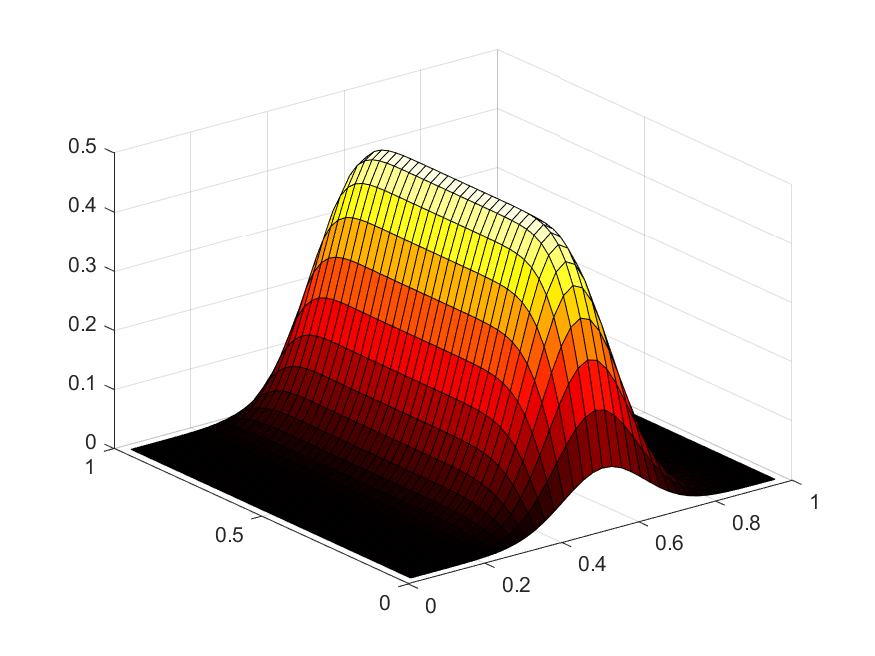
\includegraphics[width=2.5cm]{fig/rt_rst1.pdf}};
\node[draw=none,fill=none] (plot2) at (4,1.5) {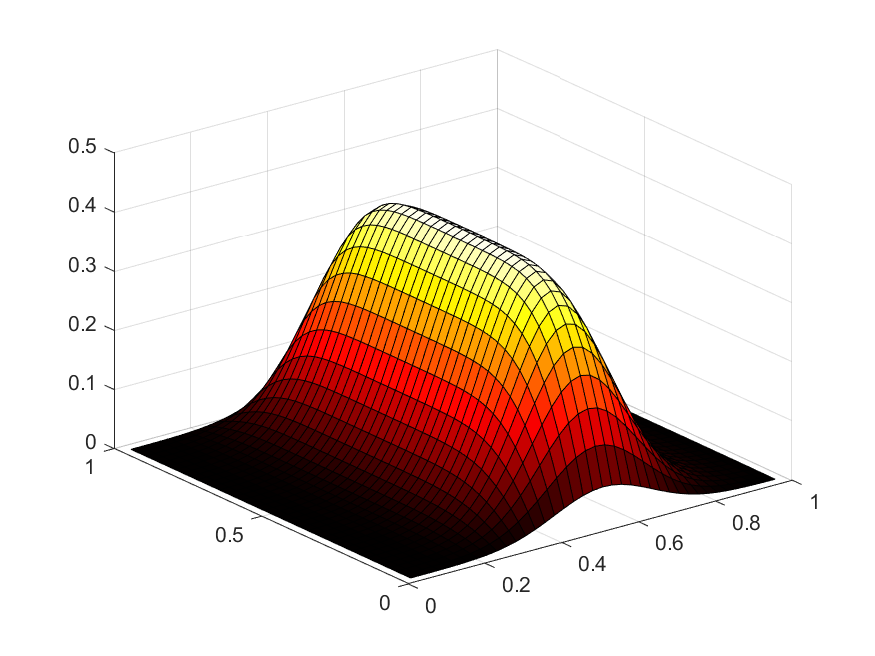
\includegraphics[width=2.5cm]{fig/rt_rst2.pdf}};
\node[draw=none,fill=none] (plot3) at (6.5,1.5) {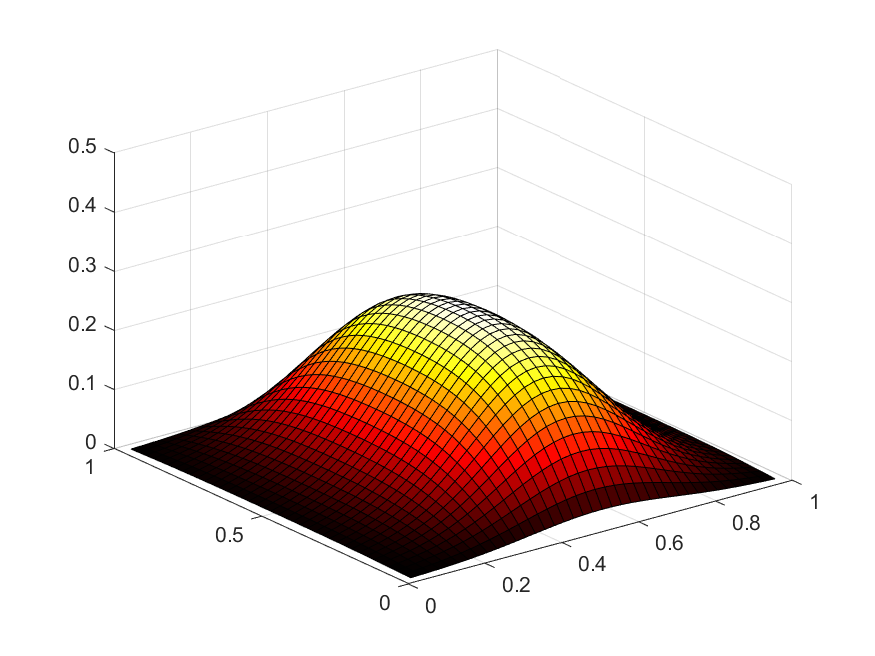
\includegraphics[width=2.5cm]{fig/rt_rst3.pdf}};
\node[draw=none,fill=none] (plot4) at (9,1.5) {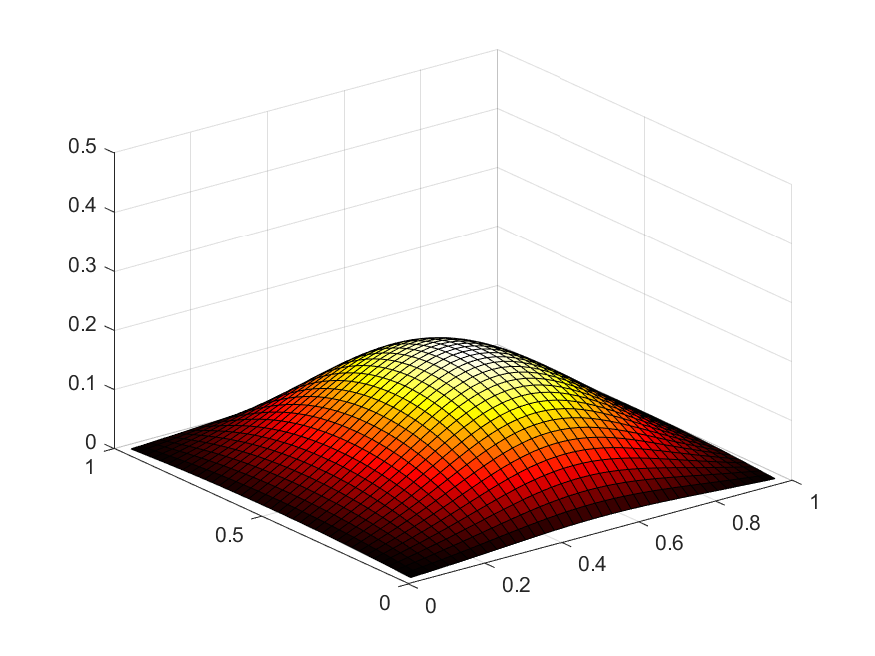
\includegraphics[width=2.5cm]{fig/rt_rst4.pdf}};
\node[draw=none,fill=none] (plot5) at (11.25,1.5) {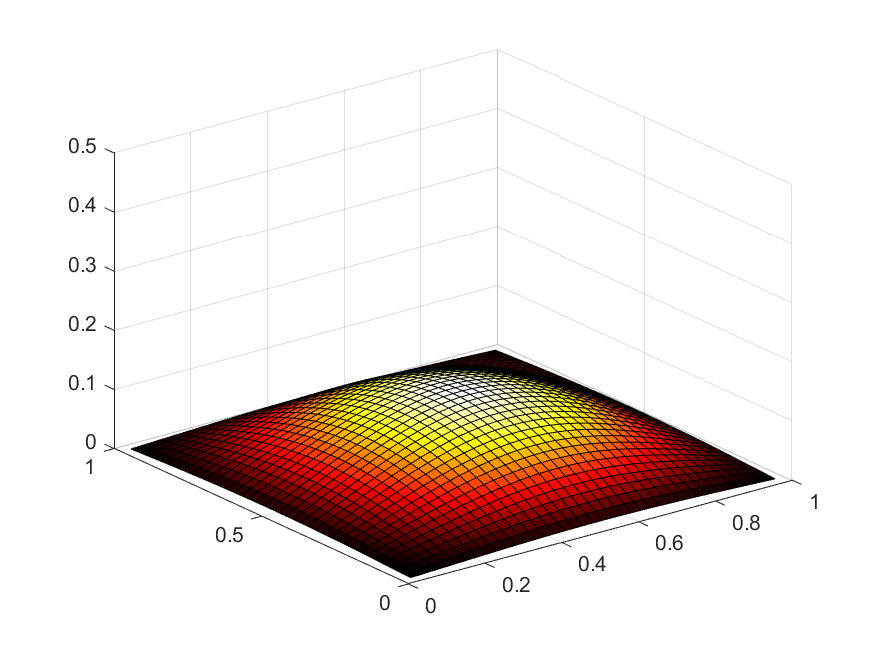
\includegraphics[width=2.5cm]{fig/rt_rst5.pdf}};

\draw[black, very thick,-latex] (leftend) -- (rightend);
\draw[black, very thick,-latex,dashed] (step0) to[bend left] (step1);
\draw[black, very thick,-latex,dashed] (step1) to[bend left] (step2);
\draw[black, very thick,-latex,dashed] (step2) to[bend left] (step3);
\draw[black, very thick,-latex,dashed] (step3) to[bend left] (step4);
\draw[black, very thick,-latex,dashed] (step4) to[bend left] (step5);
\end{tikzpicture}

\caption{Schematic illustration of residual-time restarting for approximating $\exp(-A)\vb$ (reproduced from~\cite[Figure~2.2]{schw25a}).}
\label{fig:rt_rst}
\end{figure}

To find a suitable step size $t_0$, it is proposed in~\cite[Section~2.3]{bokn20} to monitor $\beta_m(\delta_i)$ at suitably chosen sampling points $\delta_i$ in $[0,1]$. Each evaluation of $\beta_m$ requires computing the exponential of an $m \times m$ Hessenberg matrix, which therefore has about the same cost as forming the coefficient vector of the Arnoldi approximation after $m$ iterations. Thus, if $\mathcal{O}(1)$ sampling points are used for finding $t_0$, the asymptotic cost of the algorithm stays the same (and the additional amount of work is hardly noticeable for large scale problems).

As an extension,~\cite[Section~2.4]{bokn20} describes an adaptive version of the restarting procedure in which the Krylov dimension $m$ is not fixed across all cycles but is adapted on the fly for maximum efficiency by balancing the benefits of taking a larger time step against the increasing orthogonalization work.

It is also possible to generalize the RT restarting methodology to other functions than the exponential: In~\cite{bkt21}, the authors consider the inhomogeneous initial value problem $\vu^\prime(t) = -A\vu(t) + \vg,  \vu(0) = \vb$, which is solved by
\[
\vu(t) = \vb + t\varphi_1(-tA)(\vg-A\vb),
\]
and in~\cite{bks23} the second-order ODE $\vy''(t) = -A \vy(t) + \vg, \vy(0)=\vu, \vy'(0)=\vv$, is considered, whose solution can be written as
\begin{equation*}
\vy(t) = \vu + \frac12 t^2\psi(t^2 A)(-A\vu+\vg)
                    + t\sigma(t^2A)\vv,
\end{equation*}
where $\psi$ and $\sigma$ are the entire functions $\psi(x^2)=2\frac{1-\cos x}{x^2}, \sigma(x^2) = \frac{\sin x}{x}$. In the latter case, the situation becomes slightly more complicated, as the solution involves two matrix functions applied to different vectors, so two Krylov spaces (or a block Krylov subspace) need to be built. A general framework for unifying and generalizing the above approaches is given in~\cite[Section~3]{krsc26}.

\subsubsection{Multi-shift Krylov methods for rational functions in partial fraction form}\label{sec:multishift}
When $A$ is Hermitian, replacing $f(A)\vb$ by a rational function~\eqref{eq:rAb_pfe} opens another possible avenue for obtaining a limited memory Krylov method. As discussed in~\Cref{sec:rational_approximation}, this essentially reduces the approximation of $f(A)\vb$ to the solution of a family of $\ell$ shifted linear systems with $A$.

We focus our discussion here on the case that $A$ is Hermitian positive definite and all poles $\xi_i$ are real and negative (this situation arises, e.g., when using a quadrature approximation for a Stieltjes or related function), so that all systems can be solved by the conjugate gradient (CG) method~\cite{hest52}, and brief\/ly mention other possible settings at the end of this subsection.

A crucial observation that enables the efficient use of Krylov subspaces for shifted linear systems~\eqref{eq:shifted_linear_systems} is their \emph{shift invariance}
\begin{equation}\label{eq:shift_invariance}
\spK_m(A,\vb) = \spK_m(A + \xi I,\vb) \text{ for all } \xi \in \spC.
\end{equation}
Due to~\eqref{eq:shift_invariance}, a \emph{single} Krylov subspace can be used to solve all linear systems~\eqref{eq:shifted_linear_systems}, provided that one uses an initial guess resulting in collinear residuals. Commonly, one simply uses $\vx_0^{(i)} = \vnull, i = 1,\dots,\ell$.

Shift invariance of Krylov subspaces is a well-known property that has been used since the 1990s for simultaneously solving families of shifted linear systems~\cite{freu93,frgl98,frma99}, e.g., in the context of Tikhonov regularization.

It is well known that for linear systems the three-term Lanczos recurrence for the Krylov basis vectors translates into a recurrence for the Lanczos approximations~\eqref{eq:arnoldi_approximation}, so that there is no need to store the full Krylov basis $V_m$. When $A$ is Hermitian positive definite, this observation leads to the CG method, which solves a linear system requiring only a fixed storage of three vectors, independent of the number of required iterations. The crucial observation for deriving the multishift CG method presented in~\cite{frma99} is that not only the Krylov subspace enjoys the shift invariance property~\eqref{eq:shift_invariance}, but that one can also develop cheap recurrences for the iterates $\vx_m^{(i)}$ of all shifted systems, which do not require any additional matrix-vector products or inner products. To be precise, for each system beyond the first, this method requires storing two additional vectors and performing two vector additions and three vector scalings. Thus, it allows computing an approximation
\begin{equation}\label{eq:fAb_approx_multishift}
f(A)\vb \approx r(A)\vb \approx \widetilde{p}(A)\vb + \sum \omega_i\vx_m^{(i)}
\end{equation}
requiring an overall storage of $2\ell+1$ vectors. As the denominator degree required for a sufficiently accurate approximation is often rather small, this can be considered a limited memory approach in many cases. This approach was, e.g., used in~\cite{efls02} for approximating the action of the matrix sign function in lattice QCD (cf.~\Cref{sec:qcd}). For settings in which memory is very scarce, so that even $2\ell+1$ vectors cannot be stored, the authors of~\cite{efls02} propose avoiding storing the individual iterates $\vx_m^{(i)}$ of each system and instead directly assembling the combined approximation~\eqref{eq:fAb_approx_multishift} in each iteration. This way, only one additional vector per system is required, so that $\ell+2$ vectors need to be stored. This approach increases the computational cost by $\ell-1$ vector additions and $\ell$ vector scalings per iteration.

The required number of iterations of the multishift CG method is determined by the worst-conditioned system in~\eqref{eq:shifted_linear_systems}, i.e., by the one corresponding to the smallest shift. To reduce the computational cost, one can ``remove'' already converged systems from further iterations, as systems corresponding to large shifts typically require significantly fewer iterations; see, e.g.~\cite[Section~5.3]{efls02}. When $f$ is a Stieltjes function, in light of \Cref{thm:convergence_stieltjes}, one can expect the conjugate gradient method for the worst-conditioned system and the Lanczos approximation~\eqref{eq:arnoldi_approximation} for $f(A)\vb$ to require roughly the same number of iterations to reach a prescribed accuracy. The multi-shift CG method, however, has the advantage of only requiring fixed storage (at negligible computational overhead). Therefore, whenever a sufficiently accurate rational approximation of $f$ with a small number of poles is available, one can expect multishift CG to be more efficient in a limited memory setting than, e.g., using a restarted Lanczos method (which tends to exhibit delayed convergence compared to the unrestarted method). This was, e.g., also observed in the comparative study~\cite{gusc21}.

Of course, multishift Krylov methods can also be used for evaluating rational approximations of $f(A)\vb$ when $A$ is not Hermitian positive definite. E.g., when $A$ is Hermitian but indefinite, a shifted MINRES method can be used~\cite{pjed20}, and when $A$ is non-Hermitian, one can use a multishift version of a \emph{restarted} Krylov subspace method like GMRES~\cite{frgl98} or FOM~\cite{simo03}, or of a short-recurrence method like QMR~\cite{freu93} or BICGStab($\ell$). We also refer to~\cite[Section~14]{sisz06} for a general overview of multishift Krylov methods (albeit not in a matrix function context).

\subsubsection{Other limited memory techniques}\label{sec:limited_memory_other}
In the following, we summarize two further, rather specialized limited memory techniques that have appeared in the matrix function literature but do not fit into the two-pass or restarting frameworks introduced above. Both approaches require $A$ to be Hermitian.

In~\cite{casi25}, the memory requirements of the Lanczos approximation~\eqref{eq:arnoldi_approximation} are reduced by \emph{compressing} the Krylov basis using rational Krylov techniques (see~\Cref{sec:fA_rational_krylov} below for details on rational Krylov methods). In the following, assume that a sequence of poles $\vxi = (\xi_1,\xi_2,\dots,\xi_k)$ is known such that $f(A)\vb \approx r(A)\vb$ to sufficient accuracy, where $r$ is a rational function with poles $\xi_i$ (see also~\Cref{sec:fA_rational_krylov_poles} for pole selection strategies). Assume that we have performed $m+k$ Lanczos iterations, having the basis $V_{m+k} \in \spC^{(m+k) \times n}$ as well as the tridiagonal matrix $H_{m+k} \in \spC^{(m+k) \times (m+k)}$ in hand, and that we want to perform $M$ Lanczos iterations in total (where $M$ is so large that it does not fit into memory). We can then split the large Krylov basis $V_M$ tridiagonal matrix $H_M$ (which are never actually computed) as
\begin{equation}\label{eq:rational_krylov_compression_split}
V_M = [V_{m+k}, \widehat{V}] \quad\text{and}\quad H_M = \begin{bmatrix} H_{m+k} & \vb_1\ve_1^H \\ \ve_1\vb_1^H & \widehat{H} \end{bmatrix} = \begin{bmatrix} H_{m+k} & \\  & \widehat{H} \end{bmatrix}  + \begin{bmatrix} & \vb_1\ve_1^H \\ \ve_1\vb_1^H & \end{bmatrix}
\end{equation}

One then computes a basis $Q_{k} \in \spC^{(m+k)\times k}$ of the rational Krylov subspace $\spQ_k(H_{m+k}, \vb_1, \vxi)$, which only requires working with matrices and vectors of size $m+k$ and is therefore very inexpensive. One can then use the theory for low-rank updates of matrix functions~\cite{bcks21,bks18} to show that the $M$th Lanczos approximation for the rational matrix function $r(A)\vb$ is
\begin{equation}\label{eq:rational_krylov_compression_sum}
V_Mr(H_M)\ve_1\|\vb\|_2 = V_{m+k}r(H_{m+k})\ve_1\|\vb\| + \vw + \vr
\end{equation}
with
\[
\vw = -V_{m+k}Q_kr(Q_k^HT_{m+k}Q_k)Q_k^H\ve_1\|\vb\|_2
\]
and
\begin{equation}\label{eq:rational_krylov_compression_r}
\vr = [V_{m+k}Q_k, \widehat{V}] r\left(\begin{bmatrix}
    Q_k^HH_{m+k}Q_k & Q_k^H\vb_1\ve_1^H \\ \ve_1\vb_1^HQ_k & \widehat{H}
\end{bmatrix}\right)\begin{bmatrix} Q_k^H\ve_1\|\vb\| \\ \vnull \end{bmatrix}
\end{equation}
The crucial observations now are that in~\eqref{eq:rational_krylov_compression_sum}, both the $m+k$th Arnoldi approximation and the term $\vw$ can be readily computed, while only $\vr$ depends on the unknown quantities $\widehat{V},\widehat{H}$. However, in~\eqref{eq:rational_krylov_compression_r}, the Krylov basis $V_{m+k}$ computed so far only appears in the compressed form $\widetilde{V}_k := V_{m+k}Q_k \in \spC^{n \times k}$. The remainder term $\vr$ can therefore be approximated in a second cycle of the method, keeping only the compressed basis $\widetilde{V}_k$ in memory. After another $m$ Krylov steps, similar steps can be performed to refine the computed approximation, similar in spirit to the cycles of a restarted method. For the technical details, we refer the reader to the description in~\cite[Section~3]{casi25}.


Overall, we can compute an increasingly accurate approximation to $r(A)\vb$ while never keeping more than $m+k$ basis vectors in memory at the same time, and without additional operations on vectors of size $n$ compared to the standard Lanczos method. It is shown in~\cite[Section~4]{casi25}, that the approximations computed this way essentially agree with the Lanczos approximations for $f(A)\vb$, up to the error introduced by the rational approximation $r \approx f$. Thus, if $r$ is accurate enough, the method just described shows essentially the same convergence behavior as the Lanczos method, but has a greatly reduced memory footprint.

The other approach we want to highlight here, the so-called Lanczos-OR method introduced in~\cite{cgmm23}, is also intimately related to rational functions. Specifically, let $r(z) = \frac{p(z)}{q(z)}$ with polynomials $p,q$ that are coprime. Denoting by $M$ the invariance index of $\spK_m(A,\vb)$ and by $V_M, H_M$ the basis and tridiagonal matrix obtained from $M$ Lanczos steps for $A$ and $\vb$, the $m$th Lanczos-OR approximation for $r(A)\vb$ is given by
\begin{equation}\label{eq:lanczos_or}
\vf_m^{\text{OR},s} := V_m( [\widetilde{p}(H_M)]_{1:m,1:m})^{-1}\widetilde{q}(H_M)_{1:m,1:m}\ve_1,
\end{equation}
where $\widetilde{p}(z) = p(z)s(z)$ and $\widetilde{q}(z) = q(z)s(z)$  and $s$ is an arbitrary polynomial. It is shown in~\cite[Theorem~2.2]{cgmm23} that if $s$ is chosen such that $\widetilde{q}(A)$ is positive definite, the Lanczos-OR approximation is \emph{optimal} in the $\widetilde{q}(A)$-norm, i.e.,
\[
\|r(A)\vb - \vf_m^{\text{OR},s}\|_{\widetilde{q}(A)} = \min_{\vx \in \spK_m(A,\vb)} \|r(A)\vb - \vx\|_{\widetilde{q}(A)}.
\]
While the definition~\eqref{eq:lanczos_or} of the Lanczos-OR approximation involves the quantities $p(H_M)$ and $q(H_M)$, suggesting that its computation requires first running Lanczos until termination, which is of course infeasible in practice, its computation can be greatly simplified: In~\cite[Lemma~2.5]{cgmm23}, it is shown that
\begin{align*}
[\widetilde{p}(H_M)]_{1:m,1:m} &= [\widetilde{p}([H_M]_{1:m+\frac{\deg(p)}{2},1:m+\frac{\deg(p)}{2}})]_{1:m,1:m},\\
[\widetilde{q}(H_M)]_{1:m,1:m} &= [\widetilde{q}([H_M]_{1:m+\frac{\deg(q)}{2},1:m+\frac{\deg(q)}{2}})]_{1:m,1:m}.
\end{align*}
so that~\eqref{eq:lanczos_or} can be evaluated using the quantities from $m + \lceil\frac{k}{2}\rceil$ Lanczos iterations, where $k = \max\{\deg(p),\deg(q)\}$. It is then further shown in~\cite[Section~4]{cgmm23} that the approximation~\eqref{eq:lanczos_or} can be formed without explicitly storing the Krylov basis $V_{m + \lceil\frac{k}{2}\rceil}$ by employing a streaming $LDL^T$ decomposition. This way, it only requires storing $\deg(q)$ vectors in addition to three Lanczos basis vectors required for the three-term recurrence.

We note in passing that in~\cite{cgw25}, an extension of the described methodology based on the Arnoldi process for non-Hermitian matrices is considered. Due to the fact that the Krylov basis vectors do not exhibit a short recurrence in this case, it is \emph{not} possible to devise a limited memory procedure from this approach, though.

\subsection{Algorithmic enhancements}
In addition to the methods discussed in the previous subsection that directly aim to reduce the memory footprint of Krylov subspace methods, there has been work on many other algorithmic improvements for Krylov subspace methods in the last few years that aim to improve the convergence speed or reduce arithmetic cost. Many of these techniques, like preconditioning or subspace recycling, are well-established in the linear system case for many years, but present new challenges for general matrix functions.

\subsubsection{Randomized sketching}\label{sec:sketching}

\todo[inline]{KL: Should \cite{dgst26} be mentioned here?}
\todo[inline]{KL: Brand new paper \url{https://arxiv.org/abs/2608.13714}-- should see how/whether it belongs }

A rather novel approach for reducing orthogonalization cost in Krylov methods for $f(A)\vb$ is to combine them with \emph{randomized sketching}~\cite{wood14,matr20}, based on the groundwork laid in~\cite{bagr22,natr24} for linear systems and eigenvalue problems. Methods of this type can be broadly categorized into two classes: Those relying on the \emph{randomized Gram-Schmidt process}~\cite{bagr22} for cheaper orthogonalization and those that use a \emph{truncated} Gram-Schmidt process (i.e., a new basis vector is only orthogonalized against a subset of all previous basis vectors)~\cite[Algorithm~6.6]{saad00} and then use randomization in some way to stabilize the computations.

As all methods of this class primarily aim to reduce orthogonalization cost, they are mainly of interest for non-Hermitian $A$.

What all these methods have in common is that they rely on \emph{oblivious subspace embeddings}~\cite{sarl06,dmm06,wood14}. An oblivious subspace embedding is a linear mapping $S$ that embeds $m$-dimensional subspaces of $\spR^n$ into a smaller space $\mathbb{R}^s$, $s \ll n$, such that, with high probability, inner products (or norms) are distorted in a controlled manner. To be precise, $S \in \spR^{s \times n}$ is called an \emph{oblivious $(\varepsilon,\delta,m)$-subspace embedding} if, for any $m$-dimensional subspace $\mathcal{V} \subset \spR^n$, it holds with probability at least $1-\delta$ that
\begin{equation}\label{eq:sketch}
(1-\varepsilon) \| \vv \|^2 \leq \| S \vv\|^2 \leq (1+\varepsilon) \|\vv\|^2 \quad\text{ for all } \vv \in \mathcal{V}.
\end{equation}
Oblivious subspace embeddings are often constructed using probabilistic techniques, hence the name \emph{randomized sketching}. Common choices for $S$ are matrices with Gaussian entries, or for improved computational efficiency, subsampled trigonometric transforms, i.e., $S = \sqrt{\frac{s}{n}}MFD$, where $D \in \spR^{n \times n}$ is diagonal with Rademacher entries, $M \in \spR^{s \times n}$ contains $s$ randomly selected rows of the identity matrix, and $F \in \spR^{n \times n}$ is a trigonometric transform (e.g., discrete Fourier transform or Walsh--Hadamard transform). Such $S$ can be applied to a vector in $\mathcal{O}(n\log s)$ flops and is an oblivious $(\varepsilon,\delta,m)$-subspace embedding if the sketching dimension is chosen as $s = \mathcal{O}(\varepsilon^{-2}(d + \log\frac{n}{\delta})\log\frac{d}{\delta})$. In practice, one often uses a smaller sketching dimension $s = \mathcal{O}(\varepsilon^{-2}\frac{d}{\delta})$, which tends to be sufficient, except for a few academic examples; see~\cite{trop11} and section~9 of~\cite{matr20}. It is important to note that the required sketching dimension grows \emph{quadratically} in $\varepsilon$, so one must work with rather crude embedding qualities like $\varepsilon = \frac{1}{2}$.

A sketching matrix $S$ induces a semidefinite inner product $\langle \vu, \vv \rangle_S := \langle S\vu, S\vv \rangle$, which is an actual inner product when restricted to a subspace $\mathcal{V}$ for which~\eqref{eq:sketch} holds. Using this interpretation of subspace embeddings, the randomized Gram-Schmidt (RGS) process of~\cite{bagr22} can essentially be seen as a Gram-Schmidt method that employs the $\langle \cdot, \cdot \rangle_S$-inner product instead of the Euclidean inner product. One can prove that the resulting basis (which is \emph{not} orthonormal in the Euclidean inner product) is guaranteed to be extremely well-conditioned, with condition number bounded by $\sqrt{\frac{1+\varepsilon}{1-\varepsilon}}$; see~\cite[Corollary~2.2]{bagr22}. Therefore, one can expect that an Arnoldi approximation based on quantities computed with the RGS process should not deviate too much from the standard Arnoldi approximation~\eqref{eq:arnoldi_approximation}. When using this approach, inner products need only be formed between vectors of size $s \ll n$, greatly reducing the arithmetic and, in particular, the communication costs. As all other operations in the algorithm still need to be performed on vectors of length $n$, the asymptotic cost of the resulting method is the same as that of the full Arnoldi method, but it can be expected to provide a significant performance boost in highly parallel environments. This approach was used for approximating $f(A)\vb$ in~\cite[Algorithm~3.1]{ckn24}.

Another approach, first considered in the context of $f(A)\vb$ in~\cite{gusc23}, is to perform a $k$-truncated orthogonalization (i.e., only orthogonalizing a new basis vector against the $k$ previous ones) and then retrospectively orthogonalize the resulting basis with respect to the $\langle \cdot, \cdot \rangle_S$-inner product. The advantage of this approach is that it allows for arranging computations in such a way that the quadratic growth in the orthogonalization cost can be completely avoided.

Denoting by $\bar{V}_m$ the non-orthogonal basis resulting from truncated orthogonalization, the \emph{sketched FOM (sFOM) approximation} for $f(A)\vb$ is defined as
\[
\bar{\vf}_m = \bar{V}_m f\left((S\bar{V}_m)^\dagger SA\bar{V}_m\right)(S\bar{V}_m)^\dagger S\vb,
\]
where $B^\dagger$ denotes the pseudoinverse of $B$; see~\cite[Algorithm~1]{gusc23}. In~\cite{krsc26}, it is shown that in the context of matrix functions arising in the solution of an underlying ODE, this approximation can also be derived by imposing a Galerkin condition for the ODE residual with respect to the sketched inner product $\langle \cdot, \cdot \rangle_S$.

The key to stabilizing the sFOM approximation in finite precision arithmetic is to employ so-called \emph{basis whitening}, which means replacing
\[
	S\bar{V}_m \leftarrow Q_m,  \ \ {}\quad SA\bar{V}_m  \leftarrow (SA\bar{V}_m) R_m^{-1}, \ {}\quad \bar{V}_m \leftarrow \bar{V}_m R_m^{-1},
\]
where $S\bar{V}_m = Q_mR_m$ is a thin QR decomposition of the sketched basis. Using these transformations allows one to rewrite the sFOM approximation as
\begin{equation}\label{eq:sFOM}
\bar{\vf}_m = \bar{V}_m \left(R_m^{-1}f\left(\bar{V}_m^H SA\bar{V}_mR_m^{-1}\right)Q_m^H S\vb\right).
\end{equation}
It is important to note that $\bar{V}_mR_m^{-1}$ need not be formed explicitly in this formulation.\footnote{This operation alone would otherwise incur a cost of $\mathcal{O}(m^2n)$.} While this approximation often behaves remarkably similarly to the full Arnoldi method, it can also sometimes fail completely (see~\cite[Section~5]{ckn24} and~\cite[Section~5]{gusc23}), and its convergence properties are not well-understood. The analysis in~\cite{pss24} explains why one can expect the method to work similarly to full Arnoldi for entire functions like the exponential; however, understanding the behavior for functions with singularities or branch cuts remains elusive. In~\cite{gusc23}, another approximation dubbed ``sketched GMRES approximation'' (due to its reminiscence of GMRES when $f$ is the inverse) is proposed, for which it is possible to prove convergence when $f$ is a Stieltjes function and the field of values of $A$ lies in the right half plane~\cite[Theorem~3.3]{gusc23}. Unfortunately, the method is difficult to implement efficiently because it requires using numerical quadrature for complicated integrands.

We note that the transformation $\bar{V}_mR_m^{-1}$ makes the basis orthogonal in the inner product induced by $S$, and therefore, the sFOM approximation is mathematically equivalent to the approximation obtained using the RGS process. However, the behavior in floating point arithmetic can be very different, with RGS-based methods being generally more stable at the price of a higher computational cost. Another key difference between the two methodologies arises if scarce memory is an issue: Methods based on truncated Arnoldi with sketching allow for a two-pass approach (akin to the two-pass Lanczos method discussed in \Cref{sec:two_pass}), which is not possible for RGS-based methods that still require access to the full basis.

One factor that might negatively influence the behavior of the sFOM approximation is the conditioning of the non-orthogonal basis $\bar{V}_m$. This is investigated in detail in~\cite{gusi24}, which also introduces the ``sketch-and-select'' Arnoldi process: Instead of simply orthogonalizing a new basis vector against the $k$ \emph{previous} vectors, one selects any $k$ vectors from the basis to improve conditioning (e.g., based on criteria from compressed sensing). This can improve the stability of the method, but the precise influence of basis conditioning on the behavior of sFOM is not fully understood yet.

Another way to stabilize the approximation obtained from a truncated Arnoldi procedure via randomization is presented in~\cite[Algorithm~3.2]{ckn24}. It is based on the observation that the full Arnoldi approximation can be recovered from quantities computed in the truncated Arnoldi method by means of a rank-one modification of the Hessenberg matrix $\bar{H}_m$. To be precise, it holds
\[
\vf_m = \bar{V}_m f(\bar{H}_m + \bar{h}_{m+1,m}(V_{m+1}^\dagger\vv_{m+1}))\ve_1\|\vb\|,
\]
and the required vector $V_{m+1}^\dagger\vv_{m+1}$ can be obtained by solving a least-squares problem. The authors of~\cite{ckn24} propose using the randomized method Blendenpik~\cite{amt10} for this purpose, in order to obtain a method that is cheaper than the full Arnoldi method. This approach is further refined in~\cite{gkss26} and discussed from the view-point of \emph{similarity restoration}: By solving an appropriate least-squares problem, one can obtain a projected matrix that is similar to the Hessenberg matrix $H_m$ from the plain Arnoldi process and thus yields exactly the same Arnoldi approximant. As the solution of the least-squares problem can substantially increase the computational cost compared to the standard randomized Arnoldi method, it is proposed not to restore similarity in each iteration, but only, e.g., in each $10$th iteration.

Other recent uses of randomized sketching for $f(A)\vb$ can be found in the context of \emph{subspace recycling}~\cite{bugu24} (discussed in~\Cref{sec:recycling} below) as well as for stabilizing the two-sided nonsymmetric Lanczos method~\cite{siwa25}. In~\cite{gmam25}, a combination of a restarted Krylov subspace method (see \Cref{sec:restarting}) with randomized sketching is discussed, with the aim of reducing the orthogonalization cost within the individual restart cycles.

\todo[inline]{KB: mention deterministic sketching version of sFOM \cite{berg26}?}

\subsubsection{Recycling}\label{sec:recycling}
In several applications, one does not only require $f(A)\vb$ for a single matrix $A$ and a single vector $\vb$, but instead needs to compute a sequence of vectors
\begin{equation}\label{eq:sequence_fAb}
    f(A^{(i)})\vb^{(i)}, \quad i = 1,2,\dots,s.
\end{equation}
Often, the matrices $A^{(i)}$ and/or vector $\vb^{(i)}$ are not completely unrelated, but change only slowly as $i$ increases.

Typical examples of this are the solution of differential equations by exponential integrators (cf.~\Cref{sec:exponential_integrators}) and iteratively solving linear systems with the Neuberger overlap operator~\eqref{eq:overlap_operator} in lattice QCD (cf.~\Cref{sec:qcd}). In such situations, it can be beneficial to reuse some information gathered when solving one problem, in order to improve the convergence behavior for the next problem(s) in the sequence. Typically, this is done by collecting information in an augmentation space $\mathcal{U}$ (which is iteratively updated) and extracting approximations for the vectors~\eqref{eq:sequence_fAb} from the enriched spaces
\begin{equation}\label{eq:augmented_krylov_space}
\mathcal{U} + \spK_m(A^{(i)},\vb^{(i)}).
\end{equation}
Often, $\mathcal{U}$ is chosen such that it contains certain approximate eigenvectors of $A$, e.g., those corresponding to eigenvalues near a singularity of $f$, as approximately deflating these vectors can be expected to speed up convergence noticeably.

This technique is known as \emph{Krylov subspace recycling} and is well-studied for solving linear systems (see, e.g., the survey~\cite{ssk20}), but it has only recently been considered for more general matrix functions. First steps in this direction were made in~\cite{bfrs22}, where recycling techniques for shifted linear systems are transferred to the matrix function case via the Cauchy integral representation~\eqref{eq:matrix_function_cauchy}. The authors propose three different versions of a recycled Arnoldi method, of which we summarize only the one that appears to be the most stable in practice here.
Given a matrix $U$ whose columns form an orthonormal basis of $\mathcal{U}$, together with the orthonormal basis $V_m$ of $\spK_m(A,\vb)$ computed by the Arnoldi process, the augmented Krylov approximation for the shifted linear system $(zI-A)\vx(z) = \vb$ can be written as
\begin{equation}\label{eq:augmented_fom_linear_system}
    \vx_m(z) = V_m(V_m^H X_m(zI-G_m) + V_m^H R_z)^{-1}V_m^H \vb,
\end{equation}
with
\[
G_m = \begin{bmatrix} I & 0 \\ 0 & H_m \end{bmatrix},
\quad
X_m = [AU, V_m],
\quad\text{and}\quad
R_z = [z(U-AU), -h_{m+1,m}\vv_{m+1}\ve_m^H].
\]
Inserting~\eqref{eq:augmented_fom_linear_system} into the Cauchy integral formula~\eqref{eq:matrix_function_cauchy} yields the augmented Arnoldi approximation
\begin{equation}\label{eq:augmented_arnoldi}
    f(A)\vb \approx \widetilde{\vf}_m = \frac{1}{2\pi i}V_m\int_\Gamma f(z)(V_m^H X_m(zI-G_m) + V_m^H R_z)^{-1}\d z\ V_m^H \vb.
\end{equation}
Experiments reported in~\cite{bfrs22} show that~\eqref{eq:augmented_arnoldi} may yield a significantly higher accuracy than the standard Arnoldi approximation for the same number of iterations. However, a significant shortcoming of this approach, which limits the practical applicability, is that there is no closed form for the integral in~\eqref{eq:augmented_arnoldi}, so that numerical quadrature has to be employed for evaluating it. On the one hand, this introduces additional hyperparameter choices (e.g., the contour $\Gamma$ to use, the specific type of quadrature rule and the number of quadrature nodes) and on the other hand, it can induce a non-negligible computational overhead.

To overcome these problems, in the subsequent paper~\cite{bugu24}, a variant of the recycled Arnoldi method is presented which combines the recycling approach with randomized sketching (cf.~\Cref{sec:sketching}). It is based on explicitly writing the Rayleigh-Ritz approximation~\eqref{eq:rayleigh_ritz_approximation} with respect to $W_m = [V_m,U]$,
\[
\widetilde{\vf}_m = W_m f(W_m^\dagger A W_m)W_m^\dagger \vb.
\]
As evaluating this Rayleigh-Ritz approximant is computationally very demanding, it is proposed to replace the least-squares problems that are implicitly solved through the Moore-Penrose pseudoinverse by their sketched counterparts, resulting in
\[
\widehat{\vf}_m = W_m f((SW_m^\dagger) SAW_m)(SW_m^\dagger) \vb,
\]
or, after basis whitening via a QR factorization $SW_m = Q_mR_m$,
\begin{equation}\label{eq:srfom}
\widehat{\vf}_m = W_m (R_m^{-1} f(Q^HSAW_mR_m^{-1})Q_m^HS\vb).
\end{equation}
Numerical experiments in~\cite{bugu24} show that the sketched-recycled Arnoldi approximation~\eqref{eq:srfom} inherits the convergence speed-up of the approximation~\eqref{eq:augmented_arnoldi}, while at the same time being much more efficient computationally. Sometimes, a slight loss of the final attained accuracy due to the effects of sketching can be observed, but these are typically of negligible magnitude.

In addition to the recycled Arnoldi approximation,~\cite[Section~2.3]{bugu24} also presents a ``GMRES-type'' approximant for $f(A)\vb$, obtained by replacing the Rayleigh-Ritz approximation~\eqref{eq:rayleigh_ritz_approximation} by a more general Bubnov--Galerkin approximation with respect to differing search and constraint spaces.

\subsubsection{Preconditioning}\label{sec:preconditioning}
\todo[inline]{KL: Make sure \cite{ita08} is mentioned here}
\todo[inline]{MS: New paper~\cite{rami26} should probably be included here}
For the iterative solution of linear systems $A\vx = \vb$, it is common practice to use a preconditioner to speed up convergence. The basis of preconditioning is that for any invertible $M \in \spC^{n \times n}$, we have
\begin{equation}\label{eq:basic_preconditioning_relations}
(AM)^{-1} = M^{-1}A^{-1} \text{ and } (MA)^{-1} = A^{-1}M^{-1}.
\end{equation}
Therefore, instead of solving $A\vx = \vb$, one can either solve $MA\vx=M\vb$ (left preconditioning) or $AM\vu = \vb, \vx = M\vu$ (right preconditioning) in order to obtain the solution $\vx$ of the original system. If $M \approx A^{-1}$, the matrix $AM$ will have a much lower condition number than $A$, and the convergence of a Krylov method for the preconditioned system can be expected to be much faster than for the original system.

Unfortunately, a relation like~\eqref{eq:basic_preconditioning_relations} does not hold in general for functions $f$ different from the inverse, so a straight-forward adaptation of preconditioning techniques from linear systems to matrix functions is not possible. Due to this difficulty, only very little work has been done so far regarding preconditioning for matrix functions, and the available techniques are restricted to very narrow function classes.\footnote{We mention in passing that shift-invert rational Krylov techniques~\cite{mono04, esho06} have also been dubbed ``preconditioning'' in the past. We discuss these in the general framework of rational Krylov methods in \Cref{sec:fA_rational_krylov} below, though.}

Preconditioning techniques for the (inverse) square root have recently been introduced in~\cite{frst24} based on the observation that for $M$ which commutes with $A$ and $\alpha \in \spR$, it holds
\begin{equation}\label{eq:preconditioning_relations_alpha}
(AM)^{\alpha} = A^\alpha M^\alpha = M^\alpha A^\alpha
\end{equation}
if $A, M$ and $AM$ do not have eigenvalues on the nonpositive real axis. The main difference of this relation to~\eqref{eq:basic_preconditioning_relations} is that it does not hold for an arbitrary $M$, but instead, the preconditioner needs to be chosen such that it commutes with $A$. Therefore, a natural choice for the preconditioner is to take $M = p(A)$ as some polynomial in $A$. This way, instead of approximating $A^\alpha\vb$ in the Krylov space $\spK_m(A,\vb)$, one approximates it in $\spK_m(Ap(A),p(A)^{-\alpha}\vb)$, exploiting that $A^{\alpha}\vb = (Ap(A))^\alpha p(A)^{-\alpha}\vb$. An additional caveat arising from this is that $p(A)^{-\alpha}\vb$ needs to be evaluated in order to form the starting vector. To overcome this, the approach in~\cite{frst24} restricts to the inverse square root, $\alpha = -1/2$ and chooses $p(A) = (q(A))^2$ for some other polynomial in $A$, so that $p(A)^{1/2} = q(A)$ is easy to evaluate without further computations.\footnote{In principle, this approach can also be extended to $\alpha = -1/p, p > 2$.} This preconditioning approach can also be extended to the square root $A^{1/2}$ by exploiting the relation $A^{1/2}\vb = A^{-1/2}A\vb$ and it is proven in~\cite[Theorem~4.2]{frst24} that this can also be done when $A$ is singular, despite the occurrence of the inverse square root.

In order to speed up convergence, one aims at $p(A) \approx A^{-1}$, i.e., $q(A) \approx A^{-1/2}$. In~\cite[Section~5]{frst24}, several ways of determining such a polynomial are discussed (e.g., based on Chebyshev approximation or error minimization), but it turns out that it is often most effective (and conceptually simplest) to precondition the Arnoldi method by itself: One runs a small number of $d$ Arnoldi iterations for $A$ and a random starting vector $\vy$ and then uses the interpolating polynomial underlying the approximation $V_d f(H_d) \ve_1 \|\vy\|$ as preconditioning polynomial.

It is important to note that polynomial preconditioning will reduce the number of Krylov iterations required, but not the number of matrix vector products. If $q$ is of degree $d-1$, each iteration of the preconditioning method will require $2d-1$ matrix vector products with $A$ (plus $d-1$ matrix vector products for the starting vector). As $\mathcal{K}_m(p(A)A,q(A)\mathbf{b}) \subseteq \mathcal{K}_{(2d-1)(m+1)}(A,\mathbf{b})$, the standard Arnoldi method thus builds a \emph{larger} search space using the same number of matrix vector products. In this sense, polynomial preconditioning can be seen as a way to reduce the number of inner products and the memory footprint at the cost of a higher number of matrix-vector products. It is therefore particularly attractive for non-Hermitian matrices and in a highly parallel setting as a means of reducing communication.

Another way of preconditioning Krylov methods for the (inverse) square root is proposed in~\cite{pjed20} in the context of sampling from Gaussian processes, and it is restricted to this and similar applications. Instead of working with $A^{1/2}\vb$, it is proposed to use the matrix
\[
R = AM^{1/2}(M^{1/2}AM^{1/2})^{-1/2},
\]
where again, $M$ is the preconditioner. This matrix then fulfills $RR^H = A$ (instead of $R^2 = A$ as the square root would) but, for sampling purposes, the vector $R\vb$ has the same statistical properties as $A^{1/2}\vb$ and can therefore be used instead. A similar approach can be used to compute a vector that has the same statistical properties as $A^{-1/2}\vb$. When applicable, this approach is more flexible than polynomial preconditioning, as it allows the choice of an arbitrary $M$ as a preconditioner (as for linear systems). However, it cannot be used for general applications requiring the (inverse) square root, as it is not possible to efficiently retrieve the ``original'' vector $A^{1/2}\vb$ from $R\vb$.



\subsubsection{Low-rank modifications of the Hessenberg matrix}\label{sec:hessenberg_low_rank}
There are several variants of the Arnoldi method that replace~\eqref{eq:arnoldi_approximation} by
\begin{equation}\label{eq:modified_arnoldi_approximation_low_rank}
\widetilde{\vf}_m := V_m f(H_m + \vw\ve_m^H)\ve_1\|\vb\|,
\end{equation}
i.e., they use the same subspace and basis construction as plain Arnoldi, but instead of evaluating $f$ on $H_m$, they work with a rank-one modification of $H_m$. The reason for the specific structure of the rank-one term (which only alters the last column of $H_m$) is that this way, the approximation $\widetilde{\vf}_m$ again has an interpolation characterization like that of \Cref{thm:arnoldi_interpolation_characterization}; see,~\cite[Lemma~3]{efls02},~\cite[Lemma~2]{hoho05}. In fact, in~\cite[Lemma~1.4]{flss17}, it is proven that additive updates of the form $\vw\ve_m^H$ are the only ones which allow to still obtain an interpolation characterization.

Different particular methods now arise by the specific choice of $\vw$ in~\eqref{eq:modified_arnoldi_approximation_low_rank}. One approach is to aim for interpolating $f$ at \emph{harmonic Ritz values} instead of standard Ritz values (i.e., the eigenvalues of $H_m$). Harmonic Ritz pairs with respect to the search space $\spK_m(A,\vb)$ and target $\tau \in \spR$ are pairs $(\theta,\vv)$ satisfying
\[
(A-\tau I)\vv - (\theta - \tau)\vv \perp (A-\tau I)\spK_m(A,\vb);
\]
see~\cite{ppv95}. Interpolation at harmonic Ritz values can be achieved by selecting $\vw = |h_{m+1,m}|^2(H_m-\tau I)^{-H}\ve_m$ in~\eqref{eq:modified_arnoldi_approximation_low_rank}; see~\cite[Section~2]{hoho05}. This \emph{harmonic Arnoldi approximation} was first proposed for Hermitian $A$ in~\cite{efls02} for smoothing the convergence behavior of the Arnoldi method for approximating the action of the sign function in lattice QCD and later extended to non-Hermitian $A$ in~\cite{hoho05}. A further occurrence of the harmonic Arnoldi method can be found in~\cite{fgs14a}, where convergence of the restarted harmonic Arnoldi method is proved for $f$ a Stieltjes function and $A$ having spectrum in the right half plane (while the plain restarted Arnoldi method might fail to converge in this setting).

Another variant of~\eqref{eq:modified_arnoldi_approximation_low_rank} is proposed in~\cite{flss17} for Hermitian $A$. Here, the modified matrix
\[
\begin{bmatrix}
H_m & h_{m,m+1}\ve_m \\
h_{m+1,m}\ve_m^H & d_m + \theta_0
\end{bmatrix}
\]
is used, where $\theta_0 \in \spR$ and $d_m$ is the $m$th component of $\vd = h_{m+1,m}^2(H_m-\theta_0 I)^{-1}\ve_m$. To be precise, this matrix is a rank one modification of $H_{m+1}$, and its eigenvalues are the nodes of an $(m+1)$-point Gauss-Radau quadrature rule with a fixed node at $\tau_0$~\cite{gome09}. With proper choice of $\theta_0$, this approach might speed up convergence of the restarted Arnoldi method, or it might even restore convergence in cases where the standard restarted method diverges; see~\cite{fls20} for examples of this in the block setting.

Another approach, which also employs a rank-one modification of $H_{m+1}$ is described in~\cite{ers17}, with the goal to improve the Arnoldi approximation $\vf_m$ by already incorporating $\vv_{m+1}$ into its construction at the $m$th step. To do so, it is exploited that at the $m$th iteration, all necessary information for forming $\vf_{m+1}$, except the diagonal entry $h_{m+1,m+1}$ is already known (as $H_m$ is symmetric and tridiagonal). It is therefore proposed to replace $H_{m+1}$ by
\[
\widetilde{H}_{m+1} := \begin{bmatrix}
H_m & h_{m,m+1}\ve_m \\
h_{m+1,m}\ve_m^H & \widetilde{h},
\end{bmatrix}
\]
where $\widetilde{h}$ should approximate $h_{m+1,m+1}$. As a simple heuristic, \cite{ers17} suggests repeating the last diagonal entry, $\widetilde{h} = h_{m,m}$.

In~\cite{emr21}, this approach is extended to the non-Hermitian setting. In that case, all entries of the last column of $H_{m+1}$ are nonzero in general, so instead of approximating only the bottom right diagonal entry, the whole last column needs to be approximated. Several choices are explored, including an all-zero last column, $\vw = \boldsymbol{0}$ (which can only be used when $f$ is defined at $0$), a last column with one entry, $\vw = \alpha \ve_m$ or a multiple of the previous column, $\vw = \gamma \cdot H_{1:m+1,m}$ with $\gamma < 1$ (exploiting the fact that often, the entries of $H_{m+1}$ show a smooth decay along each row).


\section{Rational Krylov subspace methods} \label{sec:fA_rational_krylov}

Despite the success of polynomial Krylov subspace methods described in \Cref{sec:fA_polynomial_krylov}, there are situations in which the approximation quality of polynomials is limited, e.g., on unbounded domains, near discontinuities, or on equispaced points \cite{tref13}.
Even in less pathological situations, the polynomial degree, i.e., the dimension $m$ of the polynomial Krylov subspace $\spK_m(A,\vb)$ required to obtain a desired accuracy of the approximation \eqref{eq:arnoldi_approximation} may be impractically large.

In this section, we discuss \textit{rational} Krylov subspace methods for the approximation of $\fAb$ that leverage the superior approximation quality of rational functions.
The concept was first introduced by Ruhe in $1984$ in the context of eigenvalue problems \cite{ruhe84} but nowadays also finds application in matrix function approximation, cf.~the $2013$ review article \cite{gutt13} as well as the monographs \cite{gutt10,berl17,rine24}.

\begin{definition}\label{def:rat_krylov_space}
    \begin{sloppypar}
    The rational Krylov subspace of dimension $m$ of a matrix \mbox{$A\in\spC^{n\times n}$} and a vector $\bm{b}\in\spC^n$ is defined as
    \end{sloppypar}
    \begin{equation}
    \spQ_m(A,\bm{b}) = q_{m-1}(A)^{-1} \spK_m(A,\bm{b}) = q_{m-1}(A)^{-1} \spn\{ \bm{b}, A\bm{b}, A^2\bm{b}, \dots, A^{m-1}\bm{b} \}\label{eq:rat_krylov_subspace}
    \end{equation}
    where $q_{m-1}$ denotes the denominator polynomial, which we assume to be factored, i.e.,
    \begin{equation*}
    q_{m-1}(z) = \prod_{j=1}^{m-1} (1 - z/\xi_j).
    \end{equation*}
    The scalars $\xi_j\in\mathbb{C}\cup\{\infty\}, j=1, \dots , m-1$ denote the poles of $\mathcal{Q}_m$, which must not coincide with eigenvalues of $A$ to ensure the invertibility of $q_{m-1}(A)$.
\end{definition}

 The denominator polynomial $q_{m-1}(z)$ is typically prescribed \emph{a-priori} while the numerator polynomial is constructed from the polynomial Krylov subspace $\spK_m(A,\bm{b})$ as before.
 It is clear from \eqref{eq:rat_krylov_subspace} that the maximum dimension of $\spQ_m(A,\bm{b})$ is the invariance index of $\spK_m(A,\bm{b})$.

 As for polynomial Krylov methods, one is typically interested in constructing an orthonormal basis $V_m\in\spC^{n\times m}$ of the rational Krylov subspace $\spQ_m(A,\bm{b})$, where we assume that $\spQ_m(A,\bm{b})$ has invariance index greater than $m$.
 The first computational procedure to achieve this was the rational Arnoldi method proposed by Ruhe in the context of generalized eigenvalue problems \cite{ruhe94}.
 It differs from the standard (polynomial) Arnoldi method in two ways.
 Firstly, a continuation vector is chosen as a linear combination of the previously generated basis vectors before each iteration to ensure the stability of the method \cite{begu17a}.
 Secondly, each iteration of the rational Arnoldi method incorporates one factor of the denominator polynomial $q_{m-1}$ by solving a linear system with the matrix $(I-A/\xi_j)$.
 A modern description of the rational Arnoldi method can be found in \cite[Alg.~3.1]{begu15}.

 As in the polynomial case, the rational Arnoldi method may be turned into a rational Lanczos procedure for Hermitian matrices, which constitutes a three-term recurrence that may avoid storing the full Krylov basis \cite{debu07,gutt10,pps22}.
 This approach has previously been considered computationally unattractive since it requires twice as many linear system solves as the rational Arnoldi method \cite{gutt10}.
 However, it has been shown that it is possible to combine these into one linear system solve with multiple right-hand sides and construct methods that do not require access to the rational Krylov basis \cite{pps22}.

 In the general non-Hermitian case, the introduction of the denominator polynomial leads to the rational Arnoldi decomposition taking the form
 \begin{equation}\label{eq:rational_arnoldi_decomposition}
 A V_{m+1} \underline{K_m} = V_{m+1} \underline{H_m}
 \end{equation}
 with
 \begin{equation*}
 \underline{H_m} = \begin{pmatrix}
 H_m\\
 h_{m+1,m}\bm{e}_m^H
 \end{pmatrix},
 \quad
 \underline{K_m} = \begin{pmatrix}
 I_m + H_m D_m\\
 h_{m+1,m}\xi_m^{-1}\bm{e}_m^H
 \end{pmatrix},
 \end{equation*}
 where $D_m = \diag(\xi_1^{-1}, \dots , \xi_m^{-1})$ and $H_m,K_m\in\spC^{m \times m}$ are two unreduced upper Hessenberg matrices.
 Analogously to \eqref{eq:arnoldi_approximation}, this gives rise to the rational Arnoldi approximation
 \begin{equation}\label{eq:rat_arnoldi_approximation}
 \vf_m := V_mf(V_m^H AV_m)V_m^H\vb = V_mf(V_m^H AV_m)\ve_1\|\vb\|
 \end{equation}
 to $\fAb$.
 The choice $\xi_m=\infty$ simplifies \eqref{eq:rational_arnoldi_decomposition} to $A V_m K_m = V_{m+1} \underline{H_m}$ with $K_m$ invertible.
 With the usual truncation of the right-hand side, we have $V_m^H AV_m = H_m K_m^{-1}$ and we can write \eqref{eq:rat_arnoldi_approximation} as
 $$
 \vf_m =V_mf(H_m K_m^{-1})\ve_1\|\vb\|.
 $$

 The rational Arnoldi approximation \eqref{eq:rat_arnoldi_approximation} satisfies similar exactness, interpolation, and near-optimality properties as in the polynomial case.
 \begin{theorem}[Lemma~3.1 in \cite{gutt13}]
 	Let $V_m$ be an orthonormal basis of $\spQ_m(A,\bm{b})$ obtained from $m$ steps of the rational Arnoldi method on $A$.
 	Then for any rational function $r_{m,m-1}\in q_{m-1}^{-1}\Pi_{m}$ for which $r_{m,m-1}(V_m^H A V_m)$ is defined we have
 	\begin{equation*}
 	(V_m V_m^H)r_{m,m-1}(A) \bm{b} = V_m r_{m,m-1}(V_m^H A V_m) \ve_1 \|\vb\|.
 	\end{equation*}
 	In particular, for $r_{m-1,m-1}\in q_{m-1}^{-1}\Pi_{m-1}$ we have
 	\begin{equation*}
 	r_{m-1,m-1}(A) \vb = V_m r_{m-1,m-1}(V_m^H A V_m) \ve_1 \|\vb\|,
 	\end{equation*}
 	i.e., the rational Arnoldi approximation for $r_{m-1,m-1}(A) \vb$ is exact.
 \end{theorem}

 \begin{theorem}[Theorem~3.3 in \cite{gutt13}]
 	\sloppy
 	Assume that $f(V_m^H A V_m)$ and $q_{m-1}(V_m^H A V_m)^{-1}$ are defined.
 	Then the rational function $r_{m-1,m-1}$ underlying the rational Arnoldi approximation \mbox{$\vf_m = r_{m-1,m-1}(A)\vb$} defined by \eqref{eq:rat_arnoldi_approximation} interpolates $f$ at the rational Ritz values $\Lambda(V_m^H A V_m)$.
 \end{theorem}

 \begin{theorem}[Corollary~3.4 in \cite{gutt13}]\label{thm:quasioptimality_rational}
 	Let $f$ be analytic in a neighborhood of a compact set $\Sigma \supseteq \mathcal{W}(A)$.
 	Then the rational Arnoldi approximation defined in \eqref{eq:rat_arnoldi_approximation} satisfies
 	\begin{equation*}
 	\|f(A)\bm{b} - V_m f(V_m^H A V_m) \ve_1 \|\bm{b}\| \| \leq 2 K \|\bm{b}\| \min_{r_{m-1,m-1}\in q_{m-1}^{-1}\Pi_{m-1}} \| f - r_{m-1,m-1} \|_{\Sigma}
 	\end{equation*}
 	with a constant $K\leq 11.08$.
 	If $A$ is Hermitian, the result holds even with $K = 1$ and $\Sigma \supseteq \Lambda(A) \cup \Lambda(V_m^H A V_m)$.
 \end{theorem}

 \todo[inline]{KB: to be checked whether the listed references and approaches based on error bounds from \Cref{sec:fA_rational_krylov_poles_prior} should be treated in more detail here}
 Several error bounds and estimates for the rational Krylov approximation to $f(A)\vb$ \eqref{eq:rat_arnoldi_approximation} are available in the literature, typically restricted to specific function classes.
 For the matrix exponential function, rational Krylov error expansion and estimate analogues to \eqref{eq:error_expansion_exponential_saad} and \eqref{eq:error_estimate_exponential_saad} in the polynomial Krylov case have been derived for general poles and matrices \cite{best24}.
 For matrix $\varphi$-functions, error estimates for rational Krylov methods whose equidistant poles share the same real part have been proposed for negative semi-definite matrices \cite{gock14,gogr14}.
 For Cauchy–Stieltjes and Laplace–Stieltjes functions,  error bounds are available for positive definite matrices with a focus on matrices with Kronecker structure \cite{maro20}.
 For Cauchy--Stieltjes/Markov functions of symmetric matrices by linking the matrix function error to that of a shifted linear system in the same subspace \cite{simu24}.
 In \cite{maro26}, error formulas for block rational Krylov approximations to $f(A)B$ are derived for general poles and matrices.
 In \cite{bcks21}, a block rational Krylov approach for approximating low-rank updates for various matrix function classes and general matrices is proposed and analyzed.

 The efficiency of rational Krylov approximations mainly hinges on two ingredients: the choice of poles and the efficiency of solving the sequence of shifted linear systems.
 After briefly discussing some special cases of rational Krylov subspaces in \Cref{sec:fA_rational_krylov_SI_ext}, we review various pole selection strategies in \Cref{sec:fA_rational_krylov_poles}.
 This is a crucial ingredient since it defines the space of rational functions available for approximating the function $f$ on its rational Ritz values.
 The superior approximation quality of rational Krylov subspaces comes at the cost of having to solve a linear system in each Krylov iteration.
 As this is typically accomplished by iterative methods, this is referred to as inner iteration while the rational Krylov method for matrix function approximation acts as outer iteration.
 In \Cref{sec:fA_rational_krylov_inner_outer}, we discuss direct and preconditioned iterative solvers for the inner iteration as well as inexact approaches, which offer the potential of efficiency gains.



 \subsection{Shift-and-invert and extended Krylov methods}\label{sec:fA_rational_krylov_SI_ext}
 \todo[inline]{SG: should we have a dedicated section about shifting? KB: \Cref{sec:fA_rational_krylov_poles} also contains pole optimization results for shift-and-invert}

Two special cases of the general rational Krylov framework introduced in the previous section are shift-and-invert and extended Krylov subspace methods, which we briefly discuss below.

What is nowadays commonly referred to as shift-and-invert Krylov method has been independently introduced by Moret and Novati as \emph{restricted denominator} rational approximations \cite{mono04} and Van Den Eshof and Hochbruck as \emph{preconditioning} Lanczos approximations \cite{esho06}.
Interestingly, both works focused on the matrix exponential, which is, e.g., central for the efficiency of the exponential integration of ODEs, cf.~\Cref{sec:exponential_integrators}.

The basic idea behind shift-and-invert Krylov methods is that all poles of the rational Krylov subspace \eqref{eq:rat_krylov_subspace} coincide, i.e., $\xi=\xi_1=\dots=\xi_{m-1}$.
Moreover, a result from approximation theory dictates that this shared pole is real-valued \cite{esho06}.
From the restricted denominator approximation viewpoint, this corresponds to function approximation by the family of rational functions
$$
(I - A/\xi)^{-m+1}p_{m-1}(A),
$$
where the polynomial $p_{m-1}$ is constructed from the polynomial Krylov subspace $\spK_m(A,\bm{b})$.
The preconditioning viewpoint considers the spectral transformation induced by $(I - A/\xi)^{-1}$ that leads to rapid convergence of polynomial Krylov methods in the subspace \mbox{$\spK_m((I - A/\xi)^{-1},\bm{b})$}.
The (optimal) choice of the shift $\xi$ is discussed in \Cref{sec:fA_rational_krylov_poles}.

From a computational perspective, shift-and-invert methods have the advantage that the linear system solve in each rational Krylov iteration involves the same matrix $(I - A/\xi)$.
This is particularly attractive if it is possible to compute a matrix decomposition of $(I - A/\xi)$ such as an LU or Cholesky decomposition that subsequently allows for efficient linear system solves.
A deeper discussion of approaches for the solution of the shifted linear system can be found in \Cref{sec:fA_rational_krylov_inner_outer}.

Restarting shift-and-invert methods as discussed in \Cref{sec:restarting} for polynomial Krylov methods has been proposed for general functions and positive semi-definite matrices in \cite{mopo12}.
Moreover, residual-time restarting procedures for the matrix exponential of non-Hermitian matrices have been studied \cite{bokn20,botc21}.

Clearly, all error analyses of general rational Krylov methods apply to shift-and-invert methods.
Specialized shift-and-invert analysis is available as error bounds for the matrix exponential \cite{mono04,esho06} as well as error estimates for $\varphi$-functions \cite{gogr13,gock14}.

 \todo[inline]{KL will do EK}

 \begin{itemize}
    \item Extended Krylov~\cite{drkn98}, short recurrences/recursion relations~\cite{jare09,jare11}, two-sided~\cite{schw16a}, Hamiltonian~\cite{bfs22}
    \item Error estimates for $\varphi$-function approximation for extended Krylov~\cite{gogr13,gock14}
    \item Other things you should cite: \cite{xuxu23a, knsi10, schw16, bgjj19, bej20, jjr21} also \cite{gogr13}?
 \end{itemize}

 \subsection{Pole selection}\label{sec:fA_rational_krylov_poles}
 % Might be good to split into two types: a priori and adaptive pole section, and for each, group into function classes (focus on being user-friendly)

\todo[inline]{KL: Need a high-level intro on the basic techniques that people use, then just give a list of variations -- no need to explain in great detail}

Elements from a rational Krylov subspace $\spQ_m(A,\vb)$ can be viewed as rational functions $q_{m-1}(A)^{-1} p_{m-1}(A)$ acting on the vector $\vb$, just as elements of a polynomial Krylov subspace $\spK_m(A,\vb)$ can be viewed as polynomials $p_{m-1}(A)$ acting on $\vb$.
In the polynomial case, the Krylov approximation \eqref{eq:arnoldi_approximation} picks a quasi-optimal polynomial from $\spK_m(A,\vb)$ without requiring any input beyond $A, \vb$, and $m$, cf.~\Cref{thm:quasioptimality}.
Rational Krylov approximations \eqref{eq:rat_arnoldi_approximation} satisfy a similar quasi-optimality property, cf.~\Cref{thm:quasioptimality_rational}, however, it assumes a prescribed denominator polynomial $q_{m-1}$, i.e., the rational Krylov method additionally requires the poles $\xi_1,\dots,\xi_{m-1}$ as input.
Although some approaches for adaptive pole selection exist, the majority of the literature on rational Krylov subspace methods assumes prior pole selection.

Clearly, the choice of poles decisively impacts the quality of rational Krylov approximations.
Consequently, much research effort has been devoted to their optimal selection.
In this section, we give an overview of the main techniques employed for prior pole selection in \Cref{sec:fA_rational_krylov_poles_prior} and adaptive pole selection in \Cref{sec:fA_rational_krylov_poles_adaptive}.

\subsubsection{Prior pole selection}\label{sec:fA_rational_krylov_poles_prior}
\todo[inline]{KB: division by function classes seemed non-trivial. Divided by pole optimization technique instead and pointed to \cite{gutt13} for a function class-separated exposure as of 2013.}

\todo[inline]{KB: To be decided whether/what parts deserve further elaboration, maybe one representative for each class of approach (Zolotarev's third, RKFIT, some error bound, trapezoidal rule on the annulus)?}

By \Cref{thm:quasioptimality_rational}, the accuracy of rational Krylov approximations is directly related to the problem of uniform rational approximation of the function $f$ in a compact set $\Sigma \supseteq \mathcal{W}(A)$ enclosing the field of values of $A$.
This makes rational approximation theory a natural starting point for selecting the poles $\xi_1,\dots,\xi_{m-1}$ from a second set $\Xi\subset\overline{\mathbb{C}}\setminus\Sigma$, possibly shared for a set of parameters $T$ such as the family of exponential functions $f^\tau(z) = e^{-\tau z}$ for various time step sizes $\tau\in T$.
For general closed connected sets $\Sigma$ and $\Xi$ that do not separate the plane, the Riemann mapping theorem guarantees the existence of a conformal mapping
\begin{equation}\label{eq:conformal_mapping}
\phi: \overline{\mathbb{C}}\setminus(\Sigma \cup \Xi) \rightarrow \mathcal{A}_R,
\end{equation}
where $\mathcal{A}_R = \{z\in\mathbb{C} : 1 < |z| < R\}$ denotes an annulus around the origin \cite[Thm. 5.10h]{henr88}.
Some approaches exploit this fact by studying the underlying approximation problem on the annulus.

A useful lens to view rational approximation problems is logarithmic potential theory \cite{levin2006potential}.
We refer to \cite[Sec.~7.1-7.2]{gutt10} and \cite[Sec.~4]{gutt13} for an introduction to the connection between rational approximation theory and logarithmic potential theory.
The remainder of this section summarizes the available literature on pole optimization, organized by different pole selection techniques.
An exposition as of the year $2013$ structured by the matrix exponential, resolvent, and Markov function classes can be found in \cite[Sec.~4.1-4.3]{gutt13}.

\paragraph{Classical rational approximation problems}
Examples of classical rational approximation problems used for pole selection include uniform rational best approximations for the exponential function on the positive real line \cite{cmv69,ande81,borw83,crv84}, Leja-Bagby points \cite{bagb69}, or the rational approximation problems considered by Carath{\'e}odory and Fej{\'e}r \cite{cafe11} and Zolotarev \cite{zolo77}.
The poles of the solutions to these problems yield reasonable though not necessarily optimal pole selections for a given problem.
A Carath\'eodory--Fej\'er approach has recently been employed in \cite{almo25} to compute shared poles for linear combinations of $\varphi$-functions.
In Van Den Eshof and Hochbruck's seminal work, an asymptotic analysis of uniform rational approximation errors of $f(x)=e^{-x}$ for $x\geq 0$ leads to shifts that are inversely proportional to the Krylov subspace dimension $m$ \cite{esho06}.
Moreover, a number of works rely on formulations into Zolotarev's third problem in the complex plane \cite{dkz09,kdz09} and on the real line \cite{gush26,gush26a}.
In \cite{kdz09}, imaginary complex-conjugate poles are derived for the action of the resolvent function of positive definite matrices.
The work \cite{dkz09} introduces equidistributed sequences of real poles for the action of the exponential function on real symmetric semi-definite matrices by writing the real-valued exponential in terms of the resolvent function on the imaginary axis via the inverse Fourier transform.
Finally, the recent works \cite{gush26,gush26a} derive shared single and distinct real poles for the asymptotic best rational approximation of families of the exponential function $e^{-\tau A}$ with symmetric positive semi-definite $A$ and parameters $\tau\geq 0$.

\paragraph{Rational approximation from discrete samples}
A generally applicable option when bounds or estimates on the spectral region of $A$ are available is to sample the spectrum and apply a general-purpose method for rational approximation from discrete samples.
Algorithms such as vector fitting \cite{guse99,gust06}, rational Krylov fitting (RKFIT) \cite{begu15,begu17}, or adaptive Antoulas--Anderson (AAA) \cite{nst18,natr26} are designed specifically for this task and their approximants yield poles that can be used in rational Krylov methods.
Vector fitting and RKFIT are based on the iterative relocation of $m-1$ initially chosen poles of the denominator polynomial $q_{m-1}$, while the AAA algorithm relies on the representation of the rational function in barycentric form and sequentially increases the degree $m-1$ via greedy selection of sample points as support points.
The generalized version of the RKFIT method introduced in \cite{begu17} allows fitting rational approximants of type $(m+k-1,m-1)$ for $k\in\mathbb{N}$ with shared poles for parameter-dependent functions $f^\tau(z)$.
It is based on applying the rational Krylov method itself to a diagonal matrix sampling the spectrum of $A$.
This idea was first introduced for the exponential of positive definite matrices for optimizing a single or a few cyclically repeated real poles in the context of Maxwell's equations \cite{beg15}.

\paragraph{Approaches based on error bounds}
Some approaches for particular function classes utilize error bounds on the rational Krylov approximation as pole optimization objectives.
In \cite{bere09}, the conformal mapping \eqref{eq:conformal_mapping} alongside Faber transforms allows to study rational approximation of analytic functions in general connected compact sets of the complex plane on the unit disk.
Resulting error bounds for Markov functions are related to Blaschke products, which allows the optimization of one and two repeated as well as distinct quasi-optimal poles.
In \cite{gogr14}, the optimization of poles that are restricted to have the same real part is discussed for the approximation of $\varphi$-functions of negative semi-definite matrices.
In the context of extended Krylov methods, \cite{gogr13} discusses the choice of the single pole in shift-and-invert methods for $\varphi$-functions, where the Krylov error is related to the modulus of smoothness of the functions.
For the class of functions with the integral representation $f(x)=\int_0^\infty \frac{g(t)}{t+x}dt, x>0$, the shift is chosen by minimizing function-specific error bounds \cite{more08}.
The latter approach as well as the favorable conditioning of the matrix $(\xi I - A)$ for the choice $\xi=\sqrt{\lambda_{\min}(A)\lambda_{\max}(A)}$ is discussed in the context of fractional powers of positive definite matrices \cite{mono18}.
In \cite{kbo19}, a pole selection and update procedure is proposed for parameter-dependent exponential functions of semi-definite non-Hermitian matrices by minimizing the averaged residual norm \cite{bgh13}.

\paragraph{Approaches based on quadrature}
Another line of work relies on the poles of rational functions arising from quadrature rules.
Mapping the integrand of the Cauchy integral definition \eqref{eq:matrix_function_cauchy} of matrix functions conformally to the annulus $\mathcal{A}_R$, cf.~\eqref{eq:conformal_mapping}, allows the application of the trapezoidal rule, which yields rational approximants in partial fraction form \cite[Sec.~7.3]{gutt10}.
This procedure is discussed for functions with singularities on the negative real semi-axis such as $f(A)=A^{\alpha}$ or $f(A)=\log(A)$ in \cite{hht08}.
Moreover, Gauss–Jacobi quadrature on the spectral interval of positive definite matrices can be used to construct positive, real, and simple poles for fractional powers and fractional resolvent functions \cite{abdn19}.

\paragraph{Special cases and applications}
We summarize the previously mentioned approaches for the optimization of the single pole $\xi\in\mathbb{R}$ in shift-and-invert methods, cf.~\Cref{sec:fA_rational_krylov_SI_ext}.
These include classical rational approximation problems \cite{esho06,gush26,gush26a}, rational approximation from discrete samples \cite{beg15}, and pole optimization based on error bounds \cite{bere09,more08,gogr13,bgh13,mono18,kbo19}.

It is emphasized again that some previously described techniques optimize shared poles for the families of parameter-dependent matrix functions \cite{beg15,begu17,kbo19,gush26,gush26a} and $\varphi$-functions \cite{almo25}, respectively.

Finally, some works discuss or compare different existing pole selection techniques for specific applications.
For instance, in \cite{maro20} rational Krylov approximations with Zolotarev poles, poles from equidistributed sequences, and adaptively chosen poles are analyzed and compared for Stieltjes functions of Hermitian positive definite and Kronecker product matrices.
In \cite{bcks21}, single repeated and rational best approximation poles are discussed for the exponential, single repeated and cylindrically repeated quasi-optimal poles from Jacobi elliptic functions for Markov functions, and Zolotarev poles for the sign function.
In \cite{hano17,hano17a}, equidistributed poles are employed for the approximation of $\varphi$-functions of negative definite matrices.


\subsubsection{Adaptive pole selection}\label{sec:fA_rational_krylov_poles_adaptive}

Adaptive pole selection circumvents the problem of prior pole selection discussed in the previous section.
However, only one such approach with some subsequent generalizations has been proposed in the literature and its discussion has been limited to the matrix exponential, resolvent, and Cauchy--Stieltjes/Markov functions.

The idea was first mentioned in the context of model order reduction \cite{grim97} but only fully explored in \cite{dlz10} for matrix functions.
The latter work focuses on the approximation of $f(A)\vb=e^{tA}\vb$ for positive definite $A\in\mathbb{R}^{n\times n}$ with known extremal eigenvalues $\lambda_{\min}$ and $\lambda_{\max}$.
The problem is then shifted to the frequency domain where it takes the form of $f(A)\vb=(A+\xi I)^{-1}\vb$ on the imaginary axis.
It turns out that the residual of the rational Krylov approximation $\vf_m = V_m (V_m^H AV_m + \xi I)^{-1}\ve_1\|\vb\|$ can be written as
\begin{equation}\label{eq:adaptive_poles_residual}
\|\vb - (A+\xi I)\vf_m\| = \frac{r_{m-1}(A)\vb}{r_{m-1}(-\xi)}, \qquad r_{m-1}(z) = \prod_{j=1}^{m-1} \frac{z-\theta_j}{z+\xi_j},
\end{equation}
where $\theta_j$ are the rational Ritz values of $A$ on $\spQ_m(A,\bm{b})$.
It follows from $\theta_j\in\Sigma$ with $\Sigma=[\lambda_{\min},\lambda_{\max}]$ that the function $\frac{1}{r_{m-1}(-\xi)}$ has poles in $\Xi=-\Sigma=[-\lambda_{\max},-\lambda_{\min}]$, which makes the pole selection problem correspond to the third Zolotarev problem.
\Cref{eq:adaptive_poles_residual} suggests the objective
\begin{equation}\label{eq:adaptive_poles_objective}
\max_{\xi\in\Xi} \frac{1}{|r_{m-1}(\xi)|}
\end{equation}
and choosing the first two poles $\xi_1=\lambda_{\min}$ and $\xi_2=\lambda_{\max}$ allows the selection of $\xi_{j+1}$ via \eqref{eq:adaptive_poles_objective} once the Ritz values $\theta_1,\dots,\theta_j$ have been computed from the $j$-th rational Krylov iteration.

A generalization of the procedure to non-symmetric $A$ with simple eigenvalues is proposed in \cite{drsi11}.
The main difference to the previously discussed setting is that $\Sigma$ and $\Xi=-\Sigma$ are generally complex-valued, which is reflected in the fact that the objective \eqref{eq:adaptive_poles_objective} is maximized over the border $\partial\Xi$.
The latter only needs to be roughly estimated via the convex hull of two extremal initial poles $\xi_1$ and $\xi_2$, their complex conjugates $\xi_3=\overline{\xi_1}$ and $\xi_4=\overline{\xi_2}$, as well as the first four rational Ritz values that can be computed with $\xi_1,\dots,\xi_4$.

Further generalizations are discussed for Cauchy--Stieltjes/Markov functions of non-normal matrices $A\in\mathbb{C}^{n\times n}$ where the symmetry $\Sigma=-\Xi$ does not hold \cite{gukn11,gukn13} and for block rational Krylov approximations of the exponential and for Cauchy--Stieltjes/Markov functions acting on block vectors \cite{bbj24}.


 \subsection{Inner-outer solvers and inexact methods}\label{sec:fA_rational_krylov_inner_outer}
 % Very little specifically on matrix functions, long history for Krylov in general
 % Should touch on the idea and point to the few papers that have actually done it for matrix functions

The computational bottleneck of any rational Krylov method is the solution of the shifted linear system $(I - \xi_j A)\vx=\vb_j$ in each iteration.
Since this requires a linear system solver, rational Krylov methods are sometimes referred to as inner-outer solvers (or iterations if the linear systems are solved by iterative methods).
In this section, we discuss some considerations for the choice of inner solver including preconditioning for iterative methods and briefly touch upon inexact methods, which exploit the interplay of errors on the inner and outer level, i.e., the accuracy of matrix function approximation for inexact linear system solves.
We mention that inexact polynomial Krylov methods with inexact matrix-vector products have also been analyzed in the literature, cf.~e.g., \cite{sisz03}.

A natural point of reference for the performance of rational Krylov methods are polynomial Krylov methods, whose drawbacks in terms of computational costs and memory requirements are discussed in \Cref{sec:krylov_cost_memory}.
The main motivation for preferring rational Krylov methods over polynomial ones is that the required polynomial Krylov subspace dimension to reach a prescribed accuracy often increases drastically with the problem size (or problem parameters).
Rational approximants, in contrast, promise independence of this issue, leading to less memory requirement and an improved runtime scaling with computational advantages for large-scale problems.
However, rational Krylov methods can only be expected to yield faster runtimes if the polynomial Krylov iteration numbers are sufficiently high and the involved linear systems can be solved efficiently.

The vast literature on solving linear systems of equations can broadly be divided into direct and iterative solvers \cite{saad00,gova13}.
Direct solvers rely on computing matrix decompositions such as Cholesky or LU decompositions of $(I - \xi_j A)$ upfront in $\mathcal{O}(n^3)$ runtime and subsequently solving the linear systems efficiently via $\mathcal{O}(n^2)$ forward and backward substitution \cite{gova13}.
Shift-and-invert methods (or cyclically repeated poles) are particularly attractive in this respect since only a single (or a small number of) decompositions is required.
Direct methods solve the linear systems exactly up to rounding errors incurred by finite precision arithmetic and their efficiency and memory requirement can be minimized by upfront permutations of the rows and columns of the system matrix.
A comparison in \cite{best24} shows that the upfront cost of computing matrix decompositions amortizes within a small number of linear system solves in comparison to an iterative strategy with effective preconditioner.
However, memory restrictions render the direct approach infeasible for sufficiently large problems.

Standard iterative linear system solvers for the inner iteration such as CG, MINRES, or GMRES are based on polynomial Krylov subspaces \cite{saad00}.
They are often employed with a preconditioning strategy, cf.~\Cref{sec:preconditioning}, to circumvent the very issue of increasing polynomial Krylov subspace iterations for increasing problem sizes that is discussed above in the matrix function context.
The specific choice of preconditioner in the inner iteration of inner-outer iterative schemes has been extensively discussed for eigenvalue problems, cf.~e.g., \cite{frsp06,frsp07a,frsp09}.
In the context of matrix function approximation by rational Krylov methods, incomplete factorizations \cite{esho06,bedu12} and algebraic multigrid \cite{esho06,best24} have been employed.

\todo[inline]{KB: inexact part to be revised w.r.t.\ mathematical content}
Since iterative solvers typically use a choosable tolerance on the residual norm as stopping criterion, their use as inner solver inevitably raises the question how to choose this tolerance.
A line of work on eigenvalue problems \cite{frsp07,frsp06,frsp07a,xuxu22} and matrix equations \cite{kufr20} proposes \emph{inexact} iterations, which allow to relax the tolerance of the inner iteration as the outer iteration proceeds without adversely affecting convergence of the latter.
For matrix functions, this idea has not been explored in much detail.
For shift-and-invert methods, the idea of choosing the linear system tolerance in the inner iteration inversely proportional to the error (estimate) of the outer matrix function approximation has been discussed heuristically and verified numerically in \cite{esho06}.
Inexact shift-and-invert methods have also been discussed for the exponential of Toeplitz matrices \cite{wfw15} and Stieltjes functions of Hermitian matrices \cite{gusc21}.

For general rational Krylov methods, \cite[Sec.~6]{gutt10} analyzes the error introduced by inexactness by decomposing it into approximation and sensitivity error without explicitly discussing a strategy for adapting the inner iteration tolerance.
In \cite{hano17a}, inexact rational Krylov methods for $\varphi$-function in exponential integrators are analyzed via entry decay in the Hessenberg matrix $H_m$.

A rigorous treatment for inexact rational Krylov methods for general matrix functions has only been presented recently in \cite{xuxu23}.
It also comes to the conclusion that the inner linear system tolerance may be chosen inversely proportionally to the outer matrix function error without adversely affecting the convergence of matrix function approximation.
Clearly, such inexact approaches carry the potential for reducing the dominating cost of linear system solves in rational Krylov methods in later iterations as the accuracy of the outer iteration increases.

\section{Non-Krylov iterative methods} \label{sec:non_krylov}



\section{Bilinear forms} \label{sec:bilinear_form}
As we have seen in Sections~\ref{sec:complex_networks} and~\ref{sec:fA_kernel}, many applications require the computation of bilinear forms of the kind
\[
\vb^H f(A)\,\vb.
\]
Although this problem may appear to be a trivial application of the techniques described in the rest of this work for $f(A)\vb$, bilinear forms are in fact a different problem, with three main distinguishing properties:
\begin{itemize}
  \item methods based on short recurrences, such as the Lanczos algorithm, can be used to approximate $\vb^H f(A)\vb$ with low memory requirements, since the basis vectors need not be stored;
  \item optimality properties, such as exactness for polynomials of higher degree and sharper error bounds, can hold for $\vb^H f(A)\vb$ to a greater extent than for $f(A)\vb$;
  \item the behavior of algorithms in finite precision can differ when they are applied to bilinear forms rather than to $f(A)\vb$; see \cite{stti11} for $f(x) = x^{-1}$.
\end{itemize}
As anticipated in Section~\ref{sec:errest_integration_quadrature}, when $A$ is Hermitian, the Lanczos approximation of $\vb^H f(A)\vb$ corresponds to an $m$--point Gauss quadrature rule \cite{gome09,gome94}.
This classical result follows from two observations. First, the bilinear form is a Riemann--Stieltjes integral with respect to the spectral measure~\eqref{eq:spectral_measure}. Second, the Lanczos approximant
\( \|\vb\|^2 \ve_1^T f(H_m)\ve_1,
\)
 can be rewritten as a Gauss quadrature rule by spectral decomposition of the Jacobi matrix $H_m$. Overall, this yields the approximation
\begin{equation}\label{eq:fab:gq}
\vb^H f(A) \vb = \int_{\lmin}^{\lmax} f(z)\, \d\alpha(z) \approx \sum_{j=1}^m \omega_j f(\theta_j) = \|\vb\|^2 \ve_1^T f(H_m) \ve_1,
\end{equation}
where $(\theta_j, \vq_j)$, $j=1,\dots,m$, are the eigenpairs of $H_m$ and the weights are $\omega_j = \|\vb\|^2 \bigl(\ve_1^T \vq_j\bigr)^2$.
Note that nodes and weights need not be computed explicitly: by the equality on the right in~\eqref{eq:fab:gq}, the quadrature is obtained by computing the $(1,1)$ entry of $f(H_m)$.
The Gauss quadrature rule has the maximal possible degree of exactness, namely $2m-1$. Therefore, the approximation of $\vb^H f(A)\vb$ is exact for every polynomial of degree at most $2m-1$, which doubles the degree of exactness of the Lanczos approximation~\eqref{eq:rayleigh_ritz_approximation} of $f(A)\vb$, exact only for polynomials of degree at most $m-1$\footnote{
If the Lanczos method breaks down, the approximations
\eqref{eq:rayleigh_ritz_approximation} and \eqref{eq:fab:gq} are exact.
The same holds for the Arnoldi method.}.
The same principles can be used to define and compute other Gauss--type quadrature rules, such as the Gauss--Radau and Gauss--Lobatto rules. For certain classes of functions, these rules yield upper and lower bounds on $\vb^H f(A)\vb$ (see, e.g., \cite{bebo10}), and they can also be used to obtain error estimates (see Section~\ref{sec:errest_integration_quadrature}).

\todo{SP: I think there are some parts that are overlapping with Section \ref{sec:errest_integration_quadrature}.}
For a general integrand $f$ and a general measure~\eqref{eq:spectral_measure}, however, reliable error estimation is a hard problem.
The main difficulty is that rigorous bounds on the quadrature error involve quantities, such as the value of high--order derivatives of $f$ or information on the spectral measure, that are usually hard or impossible to evaluate in practice. Moreover, as recalled in~\cite{rst15}, it is important to remark that the difference between two consecutive Gauss approximations is known not to be a reliable error estimate in general.
The \emph{anti--Gauss} rule introduced by Laurie~\cite{laur96} can be used instead. It is an $(m+1)$--point quadrature rule whose error is equal in magnitude and opposite in sign to that of the $m$--point Gauss rule for all polynomials of degree up to $2m+1$. Consequently, if the coefficients of the expansion of $f$ in the associated orthogonal polynomials decay sufficiently fast, the difference between the anti--Gauss and the Gauss approximations provides an estimate of the Gauss error~\cite{crs99,gome09}. A generalization with $m+k$ nodes was proposed and tested in~\cite{prre15}.
A further alternative is given by the \emph{generalized averaged Gauss} rules proposed by Spalevi\'c~\cite{spal07}. These rules were used to estimate the error of the approximation~\eqref{eq:fab:gq} and extended to the non--Hermitian case in~\cite{rst15}.

The connection between the Lanczos algorithm and Gauss quadrature can be extended to non--Hermitian matrices through the non--Hermitian Lanczos method; see, e.g., \cite{gutk92,gutk94}. In this framework, the more general bilinear form $\mathbf{c}^H f(A) \vb$, with $\mathbf{c}^H\vb \neq 0$, is no longer a Riemann--Stieltjes integral, but it can be seen as a linear functional $\mathcal{L}(f)$. The matrix $H_m$ is tridiagonal, but not Hermitian, and the Gauss quadrature approximation is generalized into the form
\[ \mathcal{L}(f) = \mathbf{c}^H f(A) \vb \approx \sum_{j=1}^{q} \sum_{i=0}^{m_j-1} \omega_{i,j} f^{(i)}(\theta_j) = (\mathbf{c}^H\vb) \, \ve_1^T f(H_m) \ve_1,\]
with $q$ the number of distinct Ritz values, $m_j$ the algebraic multiplicity of $\theta_j$, and $m = \sum_{j=1}^q m_j$; see \cite{drau83,pps16,pps18,popr21}.
This extension of Gauss quadrature is also optimal in terms of polynomial approximation (matching moments), since its degree of exactness is \emph{at least} $2m-1$. In particular, the look--ahead version of the non--Hermitian Lanczos method \cite{fgn93} formally resolves the so--called \emph{serious breakdown} problem of the non--Hermitian Lanczos method, since such a breakdown corresponds to a quadrature formula with degree of exactness larger than $2m-1$ \cite{popr21}.
Note that if $H_m$ is obtained by Arnoldi method, the approximation is exact for polynomials of degree at most $m-1$.

Other Gauss--type rules for the non-Hermitian case are given in \cite{rst15,aapr21}, and Arnoldi--based rules and error analysis can be found in \cite{emr21,apr24}. Extrapolation methods can also be used for the approximation of bilinear forms \cite{fimi16a,fimi16,fmrt20}.
Rational Gauss and Gauss--type rules were introduced in~\cite{prre14,apr22}, while~\cite{pps22} proposes an implementation of the rational Lanczos method for Hermitian matrices that does not require storing the entire vector basis.
Extensions to the block case can be found in \cite{fmrr13} (Gauss and anti--Gauss), \cite{rrt16} (generalized averaged Gauss), \cite{alre19} (generalized $(m+k)$--node anti--Gauss), \cite{bej20} (by global Lanczos),\cite{bejr22} (Gauss and anti--Gauss by extended Lanczos), and \cite{zds25}(acceleration of block Gauss and
Gauss–-Radau); see also the thesis~\cite{mart12}.






\section{Methods for structured matrices}\label{sec:structured}

\todo[inline]{Keep this section as brief as possible}

\subsection{Kronecker-product variants}\label{sec:kronecker}
		\todo[inline]{Caliari, Cassini, exponential integrator stuff}
        \todo[inline]{SG}
	\begin{itemize}
		\item Kronecker-structured Krylov methods for exp, Laplace--Stieltjes and Cauchy--Stieltjes~\cite{besi16}
		\item Exponential sum approximation for fractional powers of Kronecker structured matrices~\cite{caro23}
	\end{itemize}


\subsection{Hierarchical matrix approaches}\label{sec:hierarchical}
The idea of hierarchical matrix methods is to construct a data-sparse approximation of a generally dense matrix $A$ by representing suitable matrix blocks in low-rank form within a hierarchical block structure~\cite{hack99}. This representation enables subsequent operations, such as matrix--vector products and linear system solves, to be performed with almost linear complexity in the dimension of $A$.
By means of contour integral and hierarchical matrix approximations of the resolvents $(\vz I-A)^{-1}$, hierarchical matrix techniques have been successfully employed for computing the matrix exponential~\cite{ghk02}, the matrix sign function~\cite{ghk03}, negative fractional powers and other matrix functions~\cite{ghk03a, ghk04}.
Using low-rank update formulations together with rational Krylov subspace methods, functions of hierarchically semiseparable matrices can be efficiently evaluated by a divide-and-conquer paradigm~\cite{ckm22} and, in the symmetric case, by a telescopic decomposition approach~\cite{ckr24}.

These developments focus on approximating the full matrix function $f(A)$, whereas the systematic use of hierarchical matrix techniques for directly evaluating its action on vectors remains largely unexplored.

\subsection{Toeplitz matrix approaches}\label{sec:toeplitz}
\todo[inline]{KL: Find someone to do this, or do it yourself (not high-priority)}
\begin{itemize}
    \item Shift-and-Invert methods for Toeplitz matrix exponential using the Gohberg–Semencul formula for the inner system solves \cite{lps10,wfw15}
    \item Circulant preconditioners for analytic functions of Toeplitz matrices \cite{howa18}
\end{itemize}

% \section{Trace estimation and bilinear forms} -- now an application
% \todo[inline]{MS: I'm confused. Why is this in Sec.~7 on structured matrices? Do we even want this? If yes, I could write something on this.}
% \begin{itemize}
% 	\item Should probably be a decent-sized section, as it is a big application area
% 	\item logdet equivalences
% 	\item moments; mostly point to \cite{gome10}
% 	\item Network analysis measures, Gaussian processes, etc.
% \end{itemize}

\section{High-performance computing}\label{sec:hpc}

\todo[inline]{KL: Include \cite{blan26, ckor13} here}
\todo[inline]{XL: Good idea. \cite{blan26} has been published, and the ref is updated. A paragraph is added in \emph{Parallel computing} for the two papers.}


The computation of $\fAb$ takes on a different character in high-performance computing (HPC) environments, where the matrix $A$ is typically large and sparse. A central difficulty is that explicitly forming the matrix function $f(A)$ destroys this sparsity, producing a dense matrix that is impractical to store or manipulate. For this reason, HPC approaches focus on methods that compute the vector $f(A)\vb$ directly, without ever explicitly forming the dense matrix $f(A)$, modifying the original sparse structure of $A$, or requiring its transpose $A^T$. The most effective techniques are those that access $A$ only through matrix–vector products, ensuring that memory usage scales with the number of nonzero entries in $A$.

\subsection{Parallel computing}
At the implementation level, deploying $\fAb$ solvers on modern supercomputers requires careful adaptation to heterogeneous architectures that combine multi-core CPUs, GPUs, and other accelerators. Most algorithms can be implemented by parallelizing two core sets of operations:
\begin{itemize}
	\item sparse matrix-vector multiplication (SpMV),
	\item basic vector operations such as dot products and axpy updates,
\end{itemize}

On distributed-memory systems, matrices and vectors are partitioned across compute nodes and the global solution is computed through communication using frameworks like the Message Passing Interface (MPI). Within each node, shared-memory parallelism (for instance via OpenMP) can multithread local operations, while the most compute-intensive kernels are increasingly offloaded to GPUs. In GPU-accelerated settings, it is essential to keep data resident in GPU memory throughout the computation, since frequent transfers over the PCIe bus introduce latency that can negate performance gains. At the exascale level, energy efficiency is also a key concern. Maximizing floating-point performance per watt is now as important as minimizing runtime, and load-balancing strategies must reflect both considerations.

A major challenge in scaling $f(A)\vb$ methods to large processor counts is the cost of global synchronization. For example, maintaining orthogonality in Krylov subspace methods using modified Gram–Schmidt requires inner products that, in distributed settings, involve global reductions. Each process must pause, contribute its partial result, and wait for the combined value. As the number of nodes increases, the latency of these collective operations can dominate the runtime and limit scalability. Communication-avoiding variants of methods like Arnoldi and Lanczos mitigate this issue by restructuring the computation. They generate multiple basis vectors per communication step, replacing many small synchronization points with fewer, more efficient batched exchanges.

A parallel method for computing matrix functions and their action on vectors is proposed by Blanes \cite{blan26}, in which the computation is decomposed into independent shifted linear system solves that can be solved concurrently.
The performance of algorithms based on  Leja interpolation, Taylor polynomial, and Krylov method for computing the action of the matrix exponential is compared in \cite{ckor13}.


\todo[inline]{KL: Mention low-sync paper -- not quite the same as classical communication avoidance \cite{tgt26}}
\todo[inline]{KL: Mention Hessenburg methods \cite{rato18, bejs24}}

\todo[inline]{MS: I think one thing one should discuss here is how methods based on a priori polynomial approximation (e.g., Chebyshev) are often much easier to parallelize and much more efficient than Krylov methods because they completely avoid inner products. Similarly, methods based on rational approximation in partial fraction form are embarrassingly parallel, because all linear systems can be solve independently. KL: a priori rational approximations are not necessarily easier -- you have to solve a bunch of shifted systems, meaning either some kind of complicated, recycled Krylov method or multiple LU/Cholesky factorizations}

\subsection{Mixed-precision computing}
% \todo[inline]{Do we need mixed precision tricks only on $f(A)b$, or those on $f(A)$ also worth mentioning? KL: Yes, that's fine, just keep in high level. SG: what's also more interesting is which algorithms have been successfully implemented in different precisions}

% \todo[inline]{XL will talk about mixed-precision and parallelization}
% \begin{itemize}
%     \item Basic mixed precision tricks
%     \item Basic parallelization tricks -- partial fractions, contour integrals
% \end{itemize}

Modern hardware architectures increasingly leverage low-precision to deliver exceptional arithmetic throughput at the cost of reduced numerical accuracy, which is typically insufficient for scientific computing.
In this context, mixed-precision computing has become a key strategy. By performing most computations in low precision and strategically using higher precision only where necessary, mixed-precision algorithms maintain the required accuracy while improving performance and energy
efficiency over mono-precision methods.
For recent development of mixed-precision methods in numerical linear algebra, see the surveys of Abdelfattah et al.~\cite{aabc21} and Higham and Mary~\cite{hima22}.

The potential of mixed-precision computing for $f(A)\vb$ has been demonstrated in the context of exponential time integration methods~\cite{brg23}, where a reformulation of the exponential Rosenbrock–Euler method enables the actions of the matrix-$\varphi$ functions to be safely computed in reduced precision.
In the same paper, the use of low precisions has also been attempted in some matrix--vector products of the incomplete orthogonalization process within an implementation of KIOPS~\cite{grt18}.
On the other hand, mixed-precision techniques have been developed more systematically for full matrix functions $f(A)$, including the square root \cite{gks26}, general analytic functions \cite{hili21}, and polynomial approximants to the exponential and cosine \cite{liu25}. As discussed in~\Cref{sec:intro}, however, such methods do not generally provide a practical approach to computing $f(A)\vb$.

In contrast to algorithms tailored to IEEE double-precision arithmetic, multiprecision algorithms for evaluating matrix functions to arbitrary precision have also been developed, including methods for the matrix logarithm \cite{fahi18}, matrix exponential \cite{fahi19}, matrix cosine \cite{ahl22}, and more general analytic functions \cite{hili21}.

Overall, the potential of mixed precision remains largely unexploited for large-scale $f(A)\vb$ problems. In particular, the development of systematic precision-selection strategies informed by error analysis, together with comprehensive high-performance implementations, remains an open research direction.

\section{Software} \label{sec:software}
\todo[inline]{KL: Point to Higham's 2020 catalogue and look up what's been done since 2019, as he doesn't report anything after Mar 2020}
\todo[inline]{XL}

There is extensive literature on the computation of matrix functions and their actions on vectors; we refer the reader to the recent software survey \cite{hiho20} for a comprehensive overview on software in a wide variety of languages.
We emphasize that many methods for computing the action $f(A)\vb$ reduce the original large-scale problem to the evaluation of $f(H)$, where $H$ is a dense matrix of modest dimension. Consequently, the practical performance and robustness of methods for the action depend in part on the availability of dense routines for this task.

The following list collects more recently developed algorithms that appeared after the publication of the survey \cite{hiho20}.
\begin{itemize}
    \item linear combination of matrix $\varphi$-functions: scaling and recovering algorithm~\cite{alli26}
    \item analytic matrix functions: multi-precision Schur--Parlett algorithm~\cite{hili21}
    \item matrix cosine: scaling and recovering algorithm that works in arbitrary precision~\cite{ahl22}
    \item linear combination of actions of matrix $\varphi$-functions on vectors: scaling and recovering algorithm~\cite{almo25a}
\end{itemize}


\section{Conclusions} \label{sec:conclusions}
\begin{itemize}
	\item Highlight trends over the years, particularly successful methods
	\item Highlight open issues
    \begin{itemize}
        \item Preconditioning -- point to~\Cref{sec:preconditioning} and highlight need for more research here
        \item Multigrid for $f(A)\vb$ \cite{botc23}
        \item Standalone, robust solvers
        \item Robust, efficient, and accurate error estimates
        \item Floating-point/rounding-error analysis
        \item Clear guidelines on when to use which method
        \item Methods for inverse trigonometric and inverse hyperbolic functions: only $f(A)$ approaches exist \cite{aphi16}
    \end{itemize}
\end{itemize}

\section*{Acknowledgments}
\todo[inline]{Write acknowledgments}
\begin{itemize}
    \item Thank DFG for funding f(A)bulous workshop (2023) and network (2026-present)
    \item Thank Melina's SFB for supporting October 2026 iteration of the f(A)bulous network
    \item Anyone who did use an LLM to produce text in the survey needs to disclose it below!
\end{itemize}

\section*{Declaration of generative AI and AI-assisted technologies in the manuscript preparation process}
During the preparation of this work, the authors used Copilot and Claude for copyediting and language refinement. After using these tools, the authors reviewed and edited the content as needed and take full responsibility for the content of the published article.


\todo[inline]{MF:  Make sure all references are correct, current, and uniformly formatted}
\bibliographystyle{siamplain}
\bibliography{strings,references}
\end{document}
